\chapter{Evaluation and Analysis Results}
The evaluation and analysis result chapter will provide all gathered and analyzed data from the different test runned in this thesis. The chapter is divided into different subsections for each test case. 
\section{General}
To be able to run analysis on the data gathered from the different packet capturings (pcaps) and present it in an understandable way, two different programs were used; Wireshark and VsCode with pyshark. Wireshark were used to extract numbers from the pcaps and Visual Studio Code (VS Code) was used to generate graphs from the pcaps for the events. Even tough it is possible to use Wireshark to generate the same graphs as with VS Code, VS Code was selected because it is easier to generate graphs that have the same measures to compare and they are more ascetically pleasing to look at.  
\\\\
When opening a pcap in Wireshark several statistics are possible to extract. By choosing the option of "Capture File Properties", several measures were extracted from here, such as packets, average packet size in bytes, bytes and average bytes per second. The numbers from each pcap were noted down and used as a value to compare both the events to each other and to the baseline. 
\\\\
In VS Code, python was used as the programming language as it includes the package pyshark which can be used towards tshark. Two scripts with a number of different if statements were used to generate the graphs depending on the users arguments passed to the script. The scripts only differs with if the user wants to display the graphs with number of packets or number of graphs on the y-axis. The code is displayed in its whole in appendix XXXX, and in pseudo code beneath in algorithm \ref{alg:GraphScript}. For each of the if statements, the same code block is included and are only shown once in algorithm \ref{alg:GraphScript}. The graphs are all generated with bytes and packets per 2 seconds, where the y-axis is defined in amount of packets or byts and the x-axis defined as time. 

\begin{algorithm}
\caption{Script for generating graphs}\label{alg:GraphScript}
\begin{algorithmic}[1]
        \For{Each date of event} \Comment{Graph\_function start}
            \State Extract the packets from the right pcap
            \For{Each packet in pcap}
                \State Extract packet length in byte and time or add packet count to time
                \State Display graph
            \EndFor
        \EndFor \Comment{Graph\_function end}\\
    \If{Argument 2 is Outbound} \Comment{Set display filter to outbound traffic}
        \If{Argument 1 is Netatmo}
            \State Set display filter to "wlan.sa == Netatmo MAC address"
        \ElsIf{Argument 1 is Mill}
            \State Set display filter to "wlan.sa == Mill MAC address"
        \ElsIf{Argument 1 is Nedis}
            \State Set display filter to "wlan.sa == Nedis MAC address"    
        \EndIf\\
    \ElsIf{Argument 2 is Inbound} \Comment{Set display filter to inbound traffic}
        \If{Argument 1 is Netatmo}
            \State Set display filter to "wlan.da == Netatmo MAC address"
        \ElsIf{Argument 1 is Mill}
            \State Set display filter to "wlan.da == Mill MAC address"
        \ElsIf{Argument 1 is Nedis}
            \State Set display filter to "wlan.da == Nedis MAC address"  
        \EndIf\\
    \If{Argument 3 is Shower} \Comment{Event if-cases start}
        \State Set the dates from when the events occured 
        \State Graph\_function
    \ElsIf{Argument 3 is Cooking}
        \State Set the dates from when the events occured 
        \State Graph\_function
    \ElsIf{Argument 3 is Window}
        \State Set the dates from when the events occured 
        \State Graph\_function
    \ElsIf{Argument 3 is Weekend}
        \State Set the dates from when the events occured 
        \State Graph\_function
    \ElsIf{Argument 3 is Baseline}
        \State Set the dates from when the events occured 
        \State Graph\_function
    \EndIf \Comment{Event if-cases end}
\end{algorithmic}
\end{algorithm}

\begin{table}[H]
    \centering
    \caption{Overview of system arguments for scripts}
    \begin{adjustbox}{width=1\textwidth}
    \begin{tabular}{l|l|l|}
        \cline{2-3} & \textbf{Description} & \textbf{Values}\\ \hline
        \multicolumn{1}{|l|}{\textbf{Argument 1}} & Name of device & \begin{tabular}[c]{@{}l@{}}Netatmo\\ Mill\\ Nedis\end{tabular} \\ \hline
        \multicolumn{1}{|l|}{\textbf{Argument 2}} & Which packets to include & \begin{tabular}[c]{@{}l@{}}Inbound packets and bytes\\ Outbound packets and bytes\\ Inbound and outbound packets and bytes\end{tabular} \\ \hline
        \multicolumn{1}{|l|}{\textbf{Argument 3}} & Type of event & \begin{tabular}[c]{@{}l@{}}Cooking\\ Shower\\ Window\\ Weekend\\ Baseline\end{tabular} \\ \hline
        \multicolumn{1}{|l|}{\textbf{Argument 4}} & Maximum value for y-axis, in bytes or packets & "Numeric value" \\ \hline
    \end{tabular}
    \end{adjustbox}
    \label{tab:SystemArgumentsScripts}
\end{table}

To create a file for each of the events, a time filter were applied to the pcaps and then the remaining packets exported to a separate pcap that can be opened in Wireshark or make a graph out of to analyze each specific event. The time filter has the following format:

\begin{itemize}
\item \textbf{Format:} frame.time >= "Month Date, Year "Time"" && frame.time <= "Month Date, Year "Time""//
\item \textbf{Example:} frame.time >= "Jan 08, 2023 "19:30:00"" && frame.time <= "Jan 08, 2023 "20:40:00""
\end{itemize}

In this research, each event have been carried out 15 times, but to make the pages presentable and understandable to look at, only the first 12 graphs from the events are shown. The rest of the graphs follows the same pattern as the 10 first, but will be only be added in the appendix. The same applies to when comparing baseline traffic against the events. To be able to present this in an understandable way, only 7 of each category are chosen to be added to the graphical comparison. All calculations are added directly in this chapter as it is possible to do this in a presentable way without overloading the pages. For the weekend testing, all graphs are shown. 

\section{Baseline}
The capturing of baseline traffic were conducted over the course of 10 days in the same environment as the devices were when conducting the events. During the baseline, the devices have not been affected by the specific events, such as cooking, showering or window open in the same room as the devices resides. The baseline traffic will both be used to look at standard traffic from the devices and to compare this to the events in both graphs and calculations in sub chapter 5.3-5.5. The traffic from the capture file is encrypted on layer 2 (Wi-Fi) and therefore it is not possible to extract any values from the payload of the packets. This applies to all the devices.  
\subsection{Netatmo Baseline}
\textit{Figure \ref{fig:NetatmoBaselineTotalPackets}} and \textit{\ref{fig:NetatmoBaselineTotalBytes}} shows the graphs for Netatmo Home Coach from the baseline capturing from 6th of March 2023 to 15th of March 2023. 
\begin{figure} [H]
    \centering
    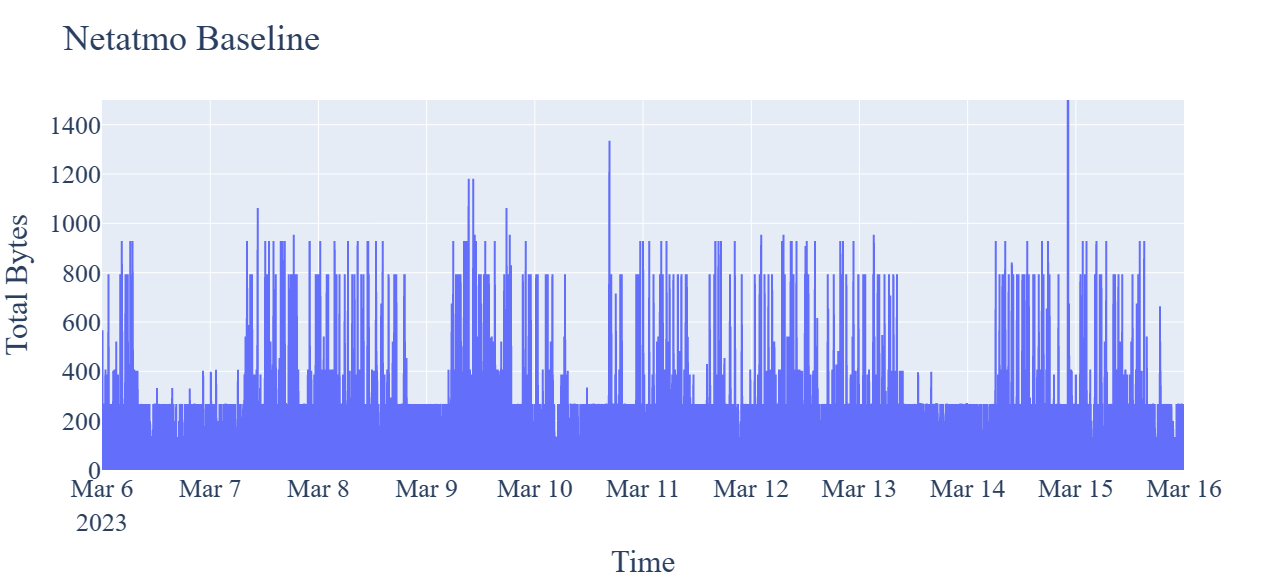
\includegraphics[scale=0.3]{figures/Netatmo_Baseline_TotalBytes.png}
    \caption{Netatmo Baseline Total Bytes}
    \label{fig:NetatmoBaselineTotalBytes}
\end{figure}

\begin{figure} [H]         
    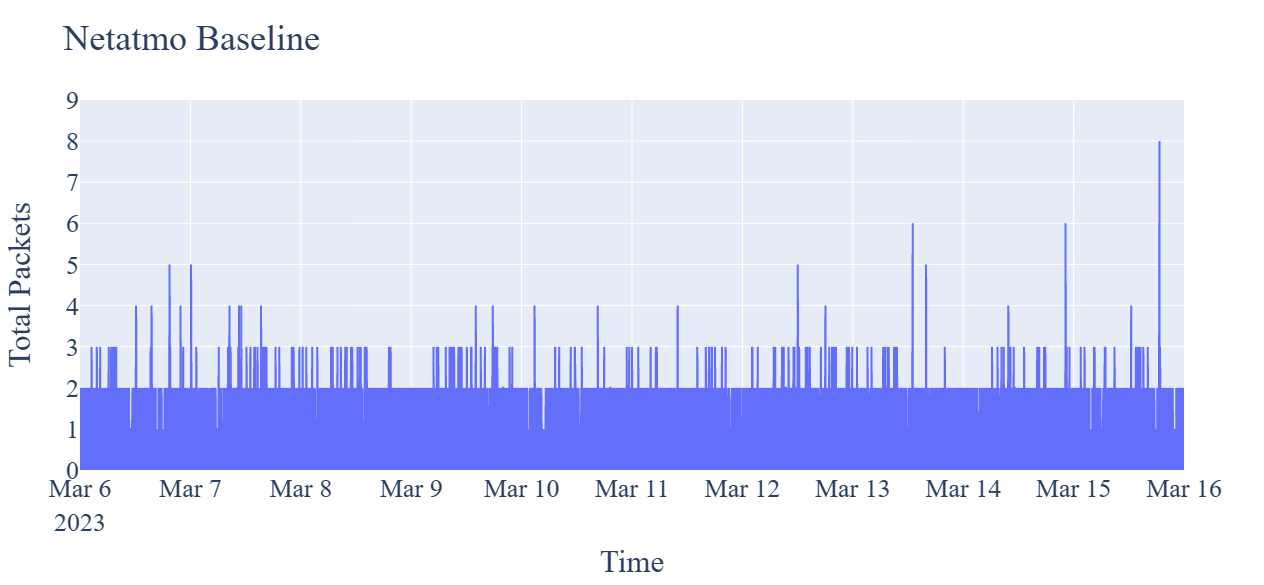
\includegraphics[scale=0.3]{figures/Netatmo_Baseline_TotalPackets.png}
    \caption{Netatmo Baseline Total Packets}
    \label{fig:NetatmoBaselineTotalPackets}
 \end{figure}

For the baseline graphs, it is possible to see that packets are sent continually at a rate of around 250 bytes per 2 seconds and 2 packets per 2 seconds. As these graphs shows the total packets and bytes sent and received, it can also be beneficial to look at what the graphs would look like if filtered on packets and bytes sent and packets and bytes received separately. 

\begin{figure}[H]
    \centering
    \begin{subfigure}[b]{0.7\textwidth}
        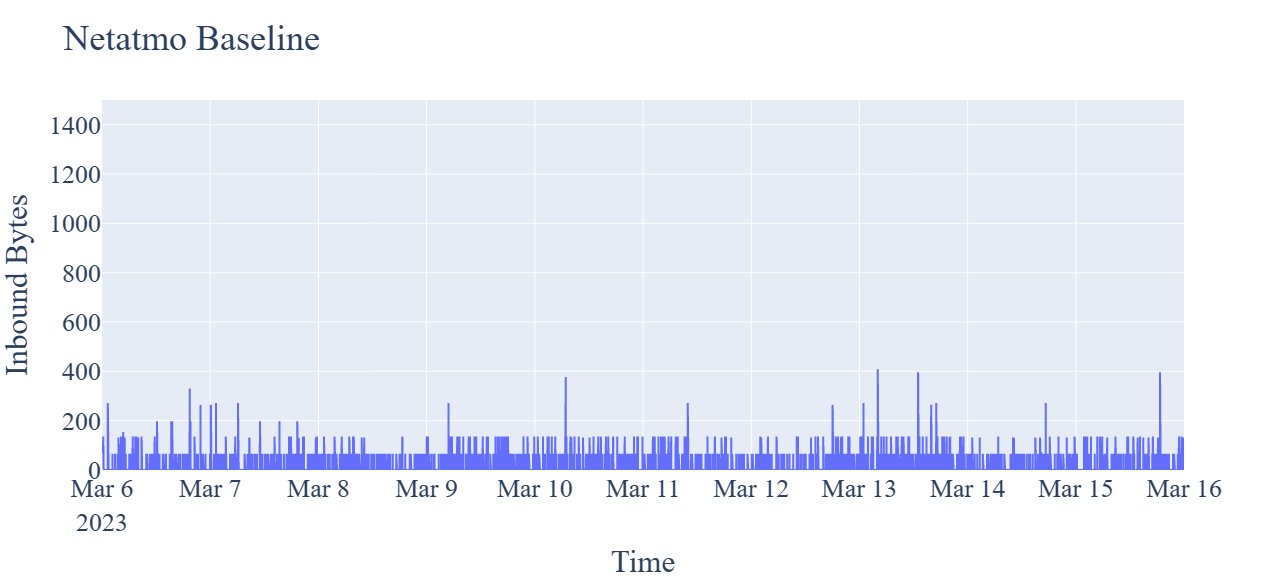
\includegraphics[width=\textwidth]{figures/Netatmo_Baseline_InboundBytes.png}
        \caption{Inbound Bytes}
        \label{fig:NetatmoBaselineInboundBytes}
    \end{subfigure}
    \begin{subfigure}[b]{0.7\textwidth}
        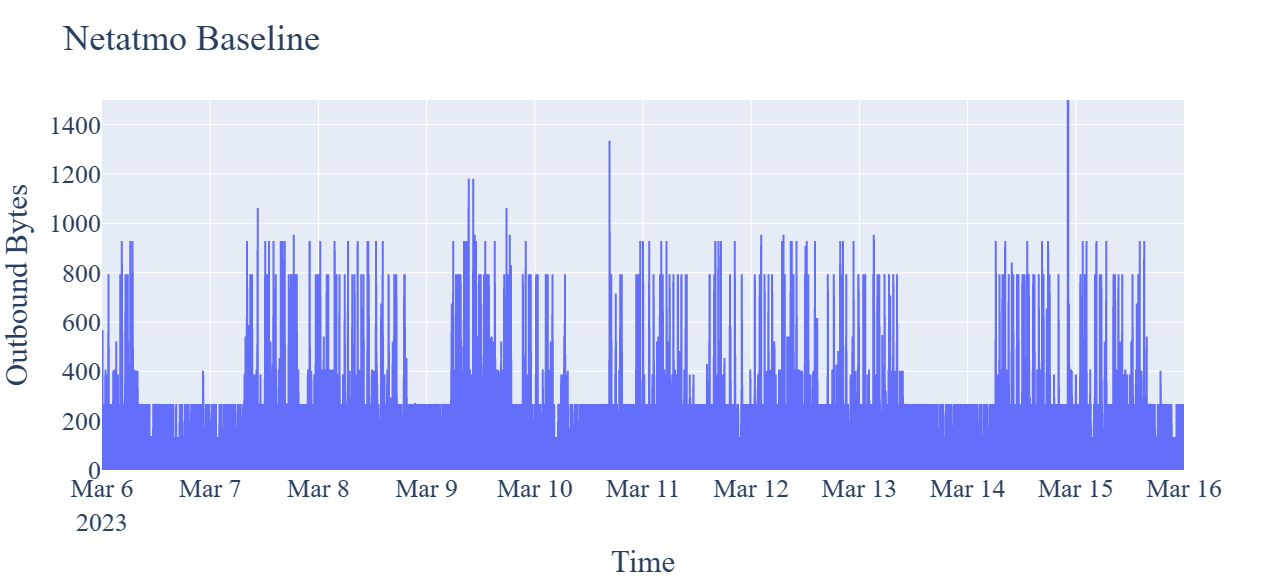
\includegraphics[width=\textwidth]{figures/Netatmo_Baseline_OutboundBytes.png}
        \caption{Outbound Bytes}
        \label{fig:NetatmoBaselineOutboundBytes}
    \end{subfigure}
    \caption{Netatmo Baseline Inbound and Outbound Bytes}
    \label{Fig:NetatmoBaselineOutandInboundBytes}
 \end{figure}

 \begin{figure}[H]
    \centering
    \begin{subfigure}[b]{0.7\textwidth}
        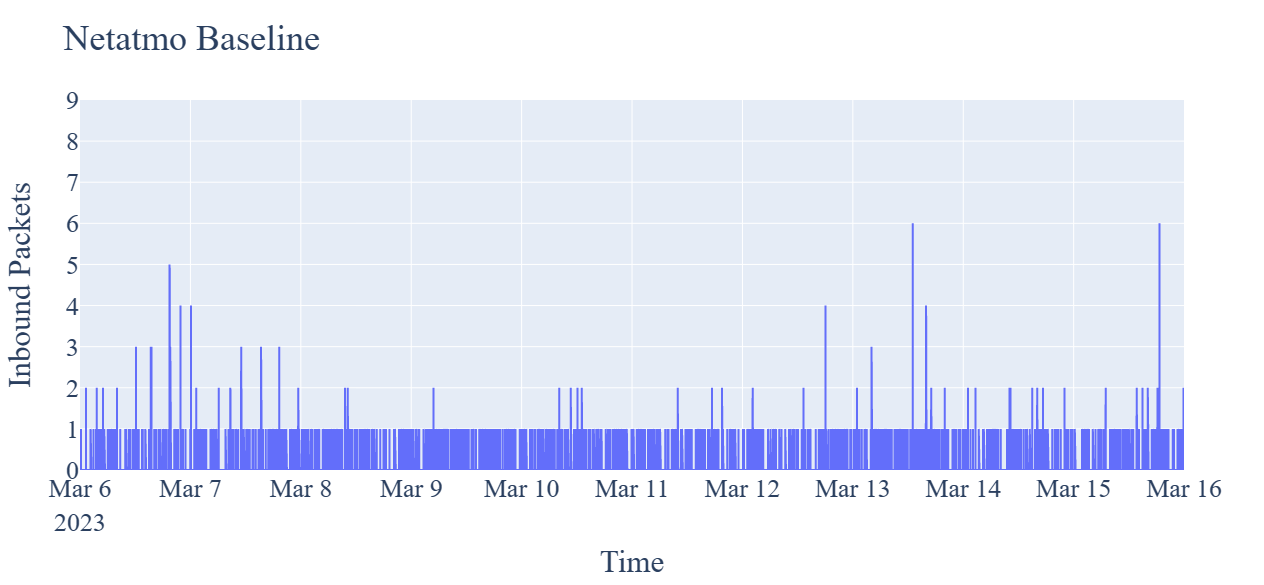
\includegraphics[width=\textwidth]{figures/Netatmo_Baseline_InboundPackets.png}
        \caption{Inbound Packets}
        \label{fig:NetatmoBaselineInboundPackets}
    \end{subfigure}
    \begin{subfigure}[b]{0.7\textwidth}
        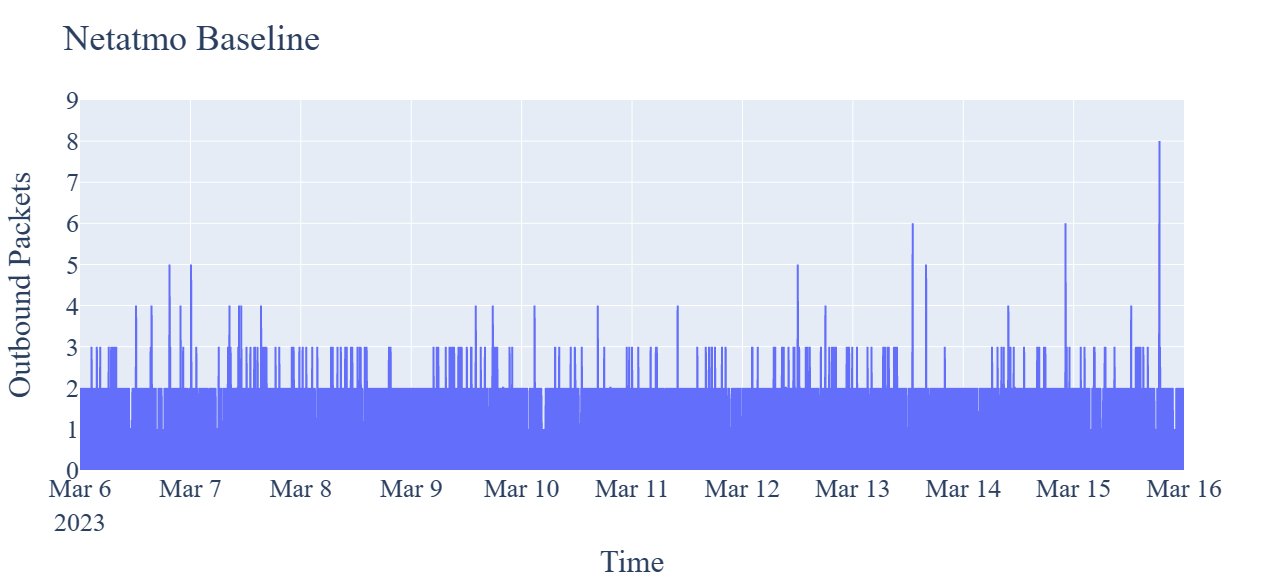
\includegraphics[width=\textwidth]{figures/Netatmo_Baseline_OutboundPackets.png}
        \caption{Outbound Packets}
        \label{fig:NetatmoBaselineOutboundPackets}
    \end{subfigure}
    \caption{Netatmo Baseline Inbound and Outbound Packets}
    \label{Fig:NetatmoBaselineOutandInboundPackets}
 \end{figure}
For the inbound and outbound bytes for Netatmo, \textit{Figure \ref{Fig:NetatmoBaselineOutandInboundBytes}}, it is clear to see that the device sends a lot more bytes than it receives. The same pattern appears in \textit{Figure \ref{Fig:NetatmoBaselineOutandInboundPackets}} for packets. Calculations made on the baseline traffic are presented in Table \ref{tab:NetatmoBaselineCalculations}. 
\begin{table}[H]
    \caption{Calculations for Netatmo Baseline Capture}
    \centering
    \begin{tabular}{ll|l|}
        \cline{3-3}                                               &                               &             \textbf{Numbers} \\ \hline
        \multicolumn{1}{|c|}{\multirow{4}{*}{\textbf{Total}}}    & Packets              & 110,735         \\ \cline{2-3} 
        \multicolumn{1}{|c|}{}                                   & Bytes                & 14,959,396       \\ \cline{2-3} 
        \multicolumn{1}{|c|}{}                                   & Average bytes/second & 17               \\ \cline{2-3} 
        \multicolumn{1}{|c|}{}                                   & Average packet size  & 135 bytes        \\ \hline
        \multicolumn{1}{|l|}{\multirow{5}{*}{\textbf{Inbound}}}  & Packets              & 1,042            \\ \cline{2-3} 
        \multicolumn{1}{|l|}{}                                   & Bytes                & 83,446           \\ \cline{2-3} 
        \multicolumn{1}{|l|}{}                                   & Average bytes/second & 0                \\ \cline{2-3} 
        \multicolumn{1}{|l|}{}                                   & Average packet size  & 80 bytes          \\ \cline{2-3} 
        \multicolumn{1}{|l|}{}                                   & Biggest packet       & 377 bytes        \\ \hline
        \multicolumn{1}{|l|}{\multirow{5}{*}{\textbf{Outbound}}} & Packets              & 109,693          \\ \cline{2-3} 
        \multicolumn{1}{|l|}{}                                   & Bytes                & 14,875,950       \\ \cline{2-3} 
        \multicolumn{1}{|l|}{}                                   & Average bytes/second & 17               \\ \cline{2-3} 
        \multicolumn{1}{|l|}{}                                   & Average packet size  & 136 bytes         \\ \cline{2-3} 
        \multicolumn{1}{|l|}{}                                   & Biggest packet       & 1,150 bytes       \\ \hline
    \end{tabular}
    \label{tab:NetatmoBaselineCalculations}
\end{table}
Comparing the inbound(Figure \ref{fig:NetatmoBaselineInboundBytes} and \ref{fig:NetatmoBaselineInboundPackets}) and outbound(Figure \ref{fig:NetatmoBaselineOutboundBytes} and \ref{fig:NetatmoBaselineOutboundPackets}) graphs with the total graphs (Figure \ref{fig:NetatmoBaselineTotalBytes} and Figures \ref{fig:NetatmoBaselineTotalPackets}), shows that the outbound graphs stands for a majority of the packets and they are very similar to the total graphs. The same is numerically shown in Table \ref{tab:NetatmoBaselineCalculations}, where over 99\% of the total packets are outbound traffic. The majority of packets sent from Netatmo are packets labeled "Data" with a size of 134 bytes, which makes up 98,3\% of the packets from the capture file. Therefore, it will be better to only display the events with graphs for total traffic to evaluate and analyze further on. 

\subsection{Mill Baseline}
\textit{Figure \ref{fig:MillBaselineTotalPackets}} and \textit{\ref{fig:MillBaselineTotalBytes}} shows the graphs for Mill from the baseline capturing from 6th of March 2023 to 15th of March 2023. 
\begin{figure} [H]
    \centering
    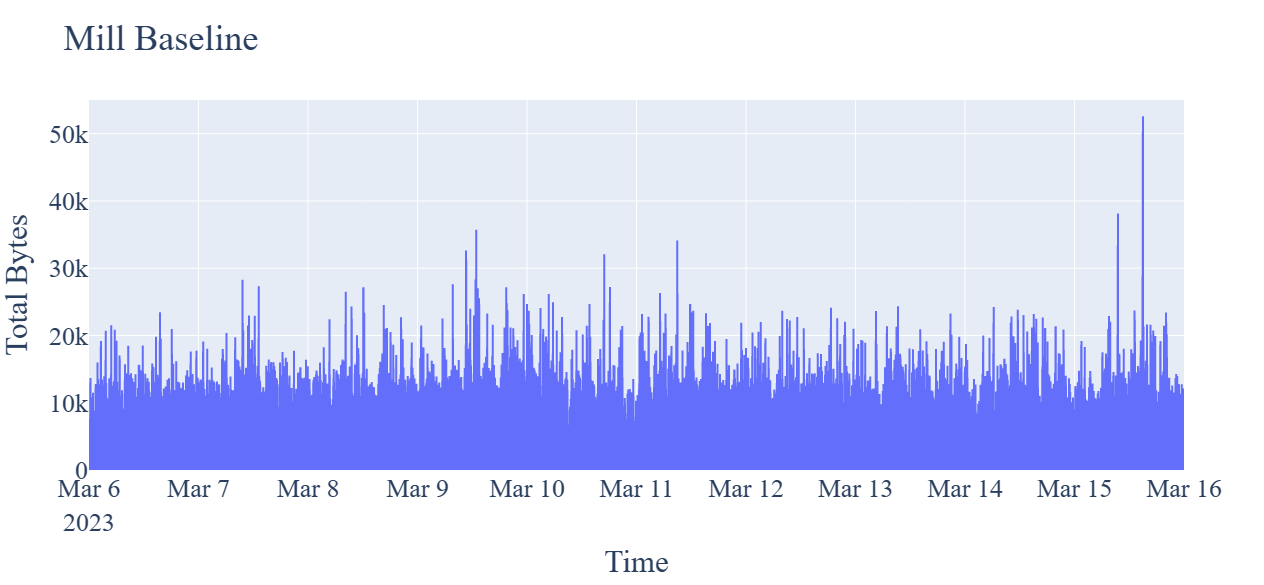
\includegraphics[scale=0.3]{figures/Mill_Baseline_TotalBytes.png}
    \caption{Mill Baseline Total Bytes}
    \label{fig:MillBaselineTotalBytes}
\end{figure}

\begin{figure} [H]
    \centering
    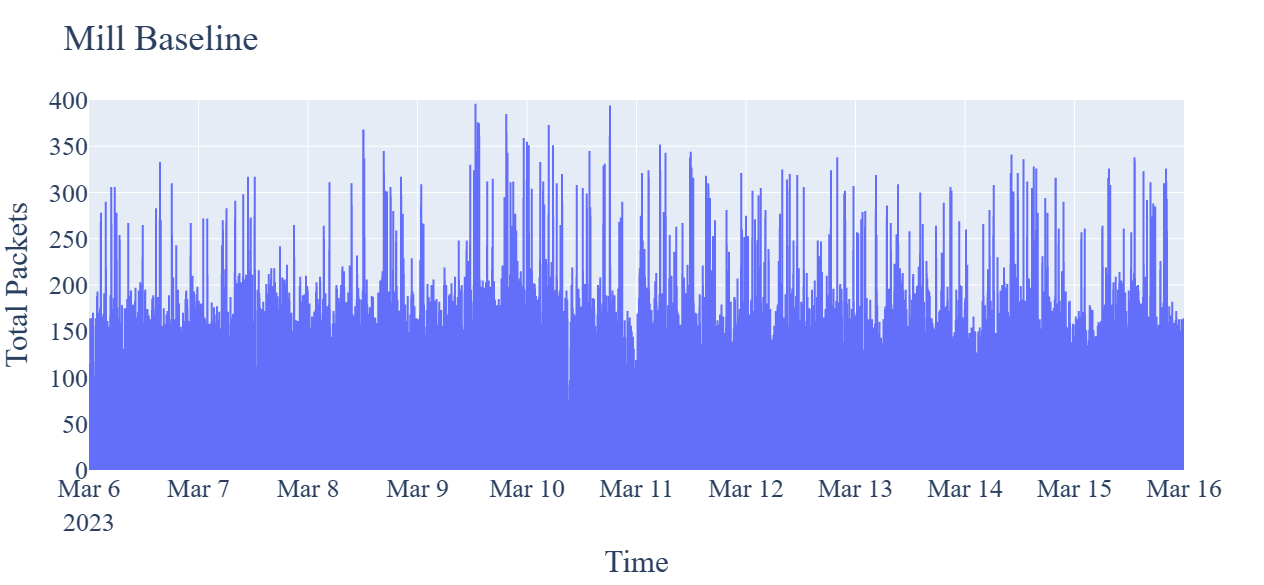
\includegraphics[scale=0.3]{figures/Mill_Baseline_TotalPackets.png}
    \caption{Mill Baseline Total Packets}
    \label{fig:MillBaselineTotalPackets}
 \end{figure}

The baseline traffic for Mill shows that the traffic varies a lot. As this device does not send live updates, but every minute, more spikes are included as it does not always send packets. It is also possible to see the spikes more clearly if the time range is smaller, this will be visible further when looking at the baseline comparison graphs for each event. 

Graphs for inbound and outbound traffic have also been made for Mill, to see the differences for the packets sent. Figure \ref{Fig:MillBaselineOutandInboundBytes} and \ref{Fig:MillBaselineOutandInboundPackets} displays the different graphs for each of the traffic directions. Numerical calculations for the baseline traffic are presented in Table \ref{tab:MillBaselineCalculations}. 

\begin{figure}[H]
    \centering
    \begin{subfigure}[b]{0.7\textwidth}
        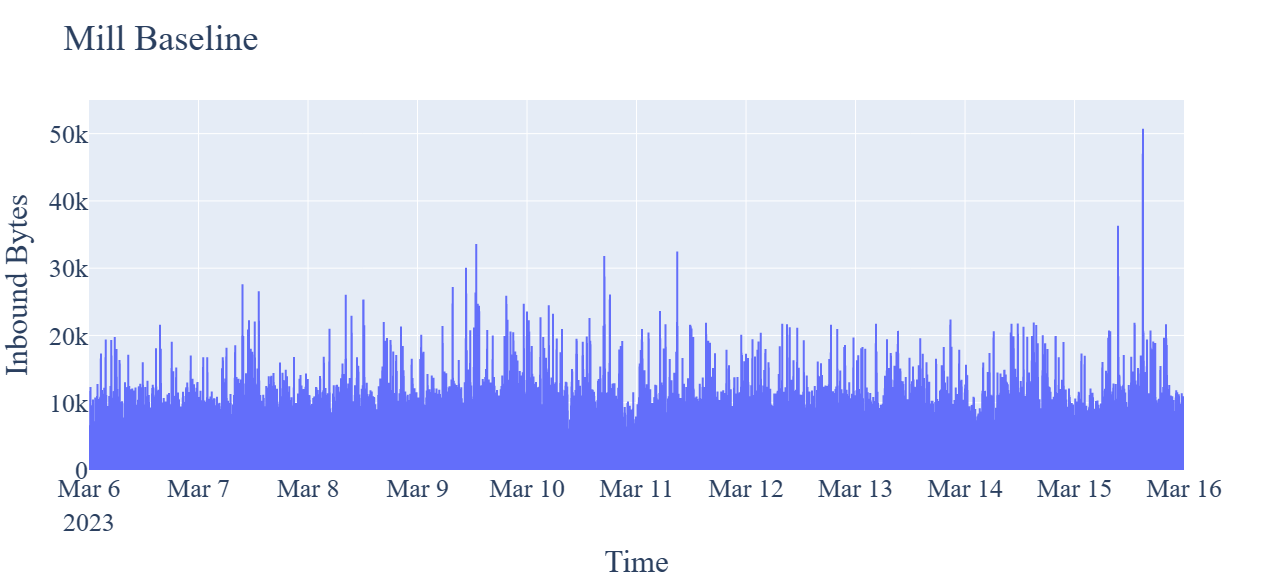
\includegraphics[width=\textwidth]{figures/Mill_Baseline_InboundBytes.png}
        \caption{Inbound Bytes}
        \label{fig:MillBaselineInboundBytes}
    \end{subfigure}
    \begin{subfigure}[b]{0.7\textwidth}
        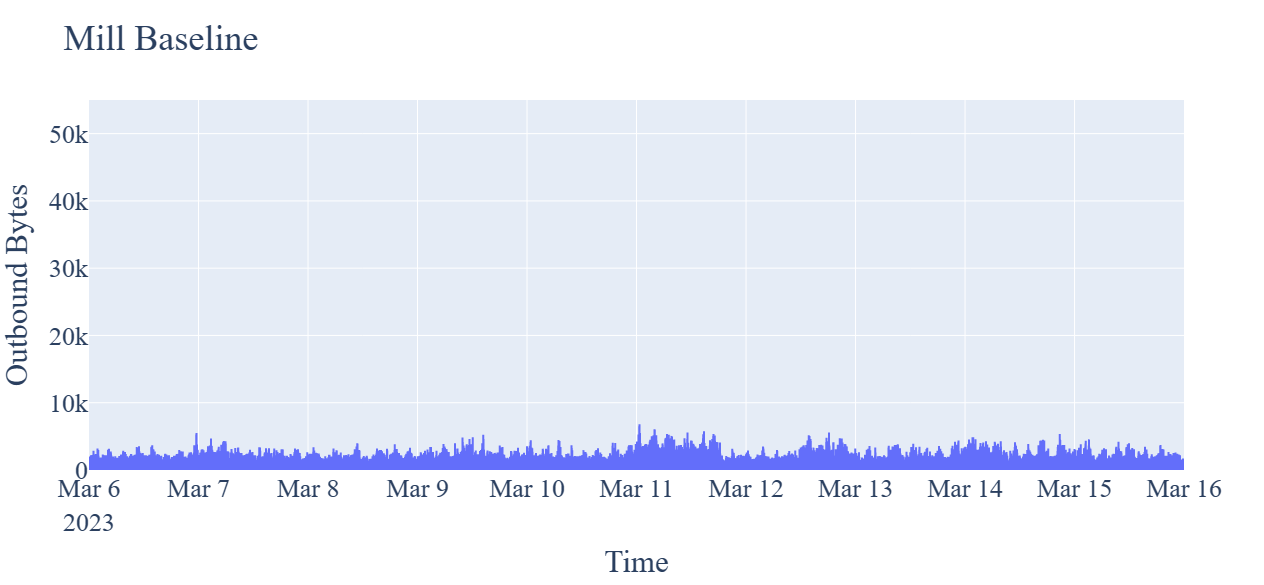
\includegraphics[width=\textwidth]{figures/Mill_Baseline_OutboundBytes.png}
        \caption{Outbound Bytes}
        \label{fig:MillBaselineOutboundBytes}
    \end{subfigure}
    \caption{Mill Baseline Inbound and Outbound Bytes}
    \label{Fig:MillBaselineOutandInboundBytes}
 \end{figure}

 \begin{figure}[H]
    \centering
    \begin{subfigure}[b]{0.7\textwidth}
        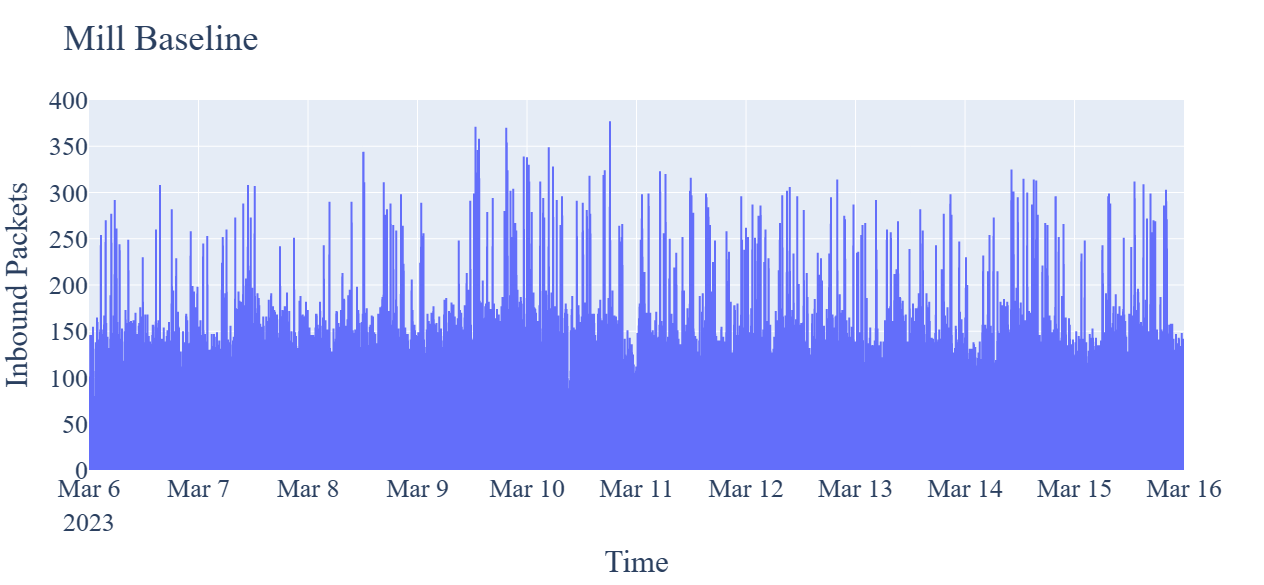
\includegraphics[width=\textwidth]{figures/Mill_Baseline_InboundPackets.png}
        \caption{Inbound Packets}
        \label{fig:MillBaselineInboundPackets}
    \end{subfigure}
    \begin{subfigure}[b]{0.7\textwidth}
        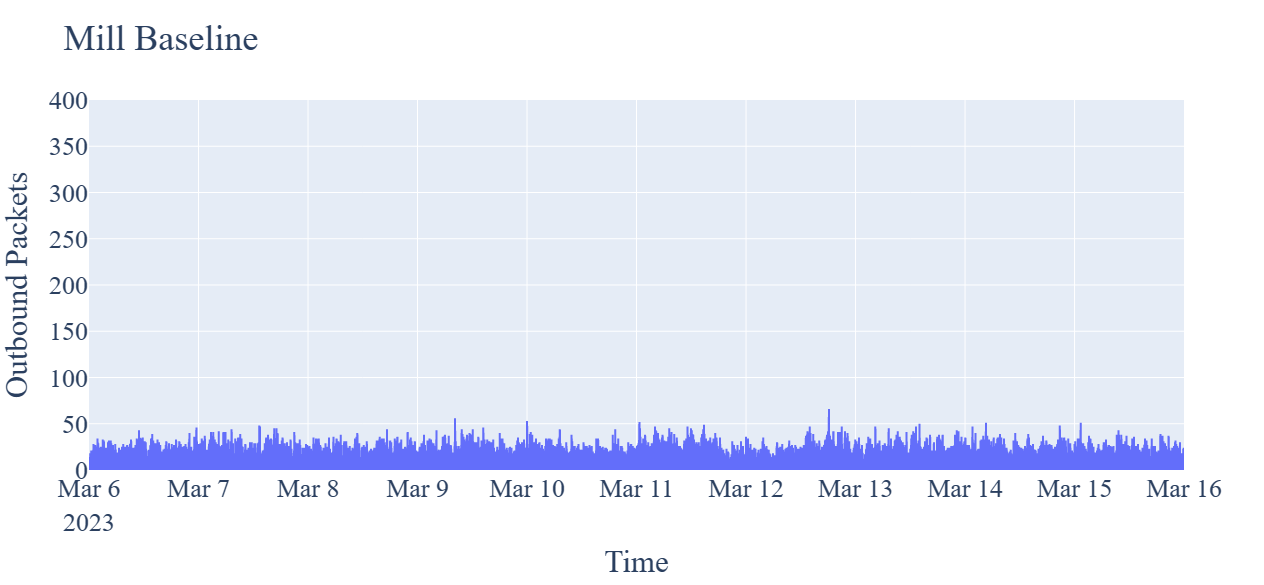
\includegraphics[width=\textwidth]{figures/Mill_Baseline_OutboundPackets.png}
        \caption{Outbound Packets}
        \label{fig:MillBaselineOutboundPackets}
    \end{subfigure}
    \caption{Mill Baseline Inbound and Outbound Packets}
    \label{Fig:MillBaselineOutandInboundPackets}
 \end{figure}

\begin{table}[H]
    \caption{Calculations for Mill Baseline Capture}
    \centering
    \begin{tabular}{ll|l|}
        \cline{3-3}                                              &                      & \textbf{Numbers} \\ \hline
        \multicolumn{1}{|c|}{\multirow{4}{*}{\textbf{Total}}}    & Packets              & 1,236,753       \\ \cline{2-3} 
        \multicolumn{1}{|c|}{}                                   & Bytes                & 129,253,290     \\ \cline{2-3} 
        \multicolumn{1}{|c|}{}                                   & Average bytes/second & 149             \\ \cline{2-3} 
        \multicolumn{1}{|c|}{}                                   & Average packet size  & 105 bytes       \\ \hline
        \multicolumn{1}{|l|}{\multirow{5}{*}{\textbf{Inbound}}}  & Packets              & 942,112         \\ \cline{2-3} 
        \multicolumn{1}{|l|}{}                                   & Bytes                & 95,458,773      \\ \cline{2-3} 
        \multicolumn{1}{|l|}{}                                   & Average bytes/second & 110             \\ \cline{2-3} 
        \multicolumn{1}{|l|}{}                                   & Average packet size  & 101 bytes       \\ \cline{2-3} 
        \multicolumn{1}{|l|}{}                                   & Biggest packet       & 1593 bytes      \\ \hline
        \multicolumn{1}{|l|}{\multirow{5}{*}{\textbf{Outbound}}} & Packets              & 294,640         \\ \cline{2-3} 
        \multicolumn{1}{|l|}{}                                   & Bytes                & 33,794,517      \\ \cline{2-3} 
        \multicolumn{1}{|l|}{}                                   & Average bytes/second & 39              \\ \cline{2-3} 
        \multicolumn{1}{|l|}{}                                   & Average packet size  & 115 bytes       \\ \cline{2-3} 
        \multicolumn{1}{|l|}{}                                   & Biggest packet       & 456 bytes       \\ \hline
    \end{tabular}
    \label{tab:MillBaselineCalculations}
\end{table}

As Figure \ref{Fig:MillBaselineOutandInboundBytes} and \ref{Fig:MillBaselineOutandInboundPackets} shows, the device receives a lot more packets and bytes than it sends off. And as the inbound graphs do not differ much from the total graphs, it will be best to proceed with the analysis in a total traffic aspect where both inbound and outbound traffic are included. This is also reflected in Table \ref{tab:MillBaselineCalculations}, which shows that 76\% of packets and 74\% of bytes are received.

\subsection{Nedis Baseline}
\textit{Figure \ref{fig:NedisBaselineTotalPackets}} and \textit{\ref{fig:NedisBaselineTotalBytes}} shows the graphs for Nedis from the baseline capturing from 6th of March 2023 to 15th of March 2023. 
\begin{figure} [H]
    \centering
    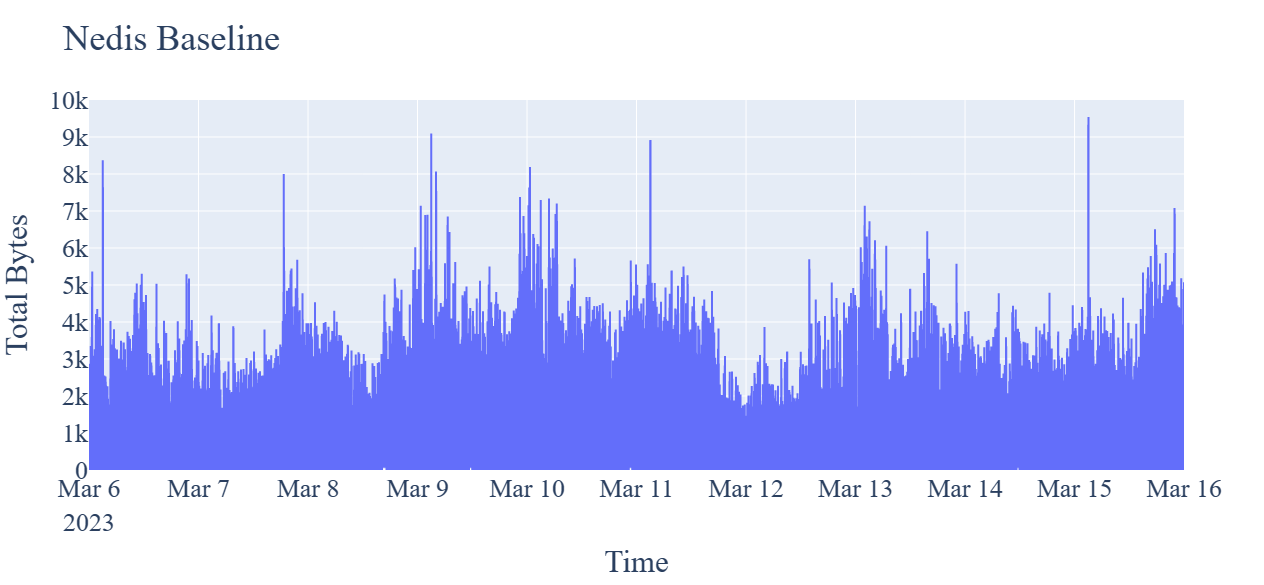
\includegraphics[scale=0.3]{figures/Nedis_Baseline_TotalBytes.png}
    \caption{Nedis Baseline Total Bytes}
    \label{fig:NedisBaselineTotalBytes}
\end{figure}

\begin{figure} [H]         
    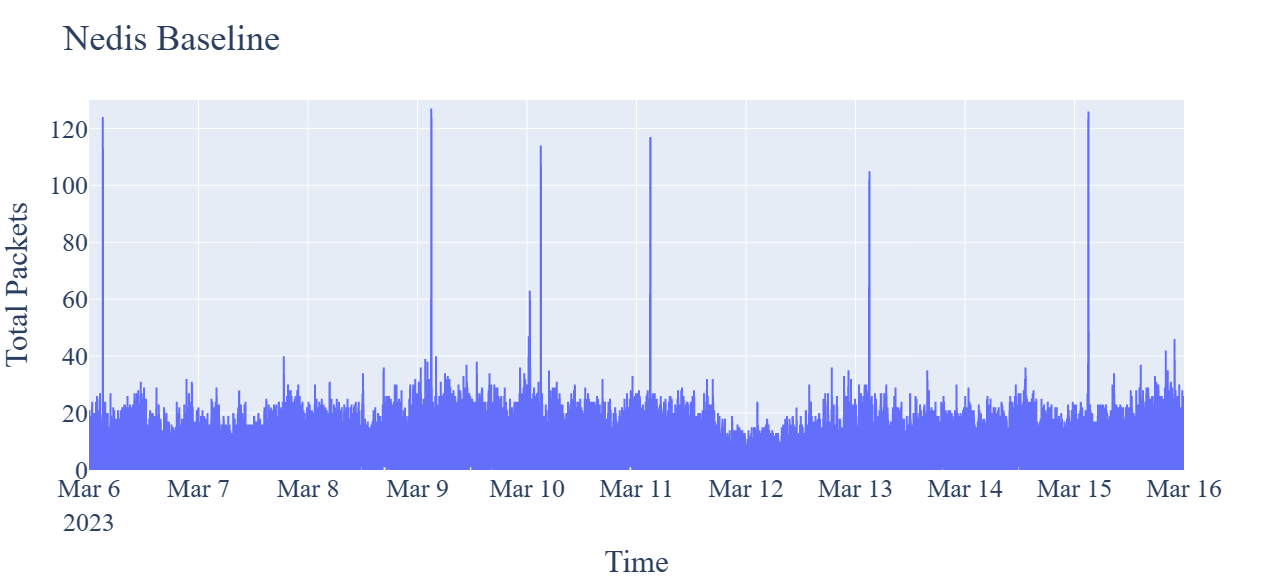
\includegraphics[scale=0.3]{figures/Nedis_Baseline_TotalPackets.png}
    \caption{Nedis Baseline Total Packets}
    \label{fig:NedisBaselineTotalPackets}
 \end{figure}

The traffic sent and received by Nedis is characterized by several spikes even though the traffic varies some. The larger spikes, which are more visible in Figure \ref{fig:NedisBaselineTotalPackets}, showing the packets, occurs almost everyday. Since traffic is encrypted, it is not possible to see what these spikes are, but for further analysis it is important to understand that normal traffic for the device, can be large spikes occurring around the same time each night the spike occurs. Even though this thesis will not go further into looking at what the spikes actually are, it can be interesting to see if they are inbound or outbound traffic. 

To look at the differences in inbound and outbound traffic for Nedis, Figure \ref{Fig:NedisBaselineOutandInboundBytes} and \ref{Fig:NedisBaselineOutandInboundPackets} are displayed. Figure \ref{fig:NedisBaselineOutboundPackets} shows that the spikes are packets which the device receives.
Even though the graphs for inbound and outbound traffic from Nedis looks more similar, the calculations presented in Table \ref{tab:NedisBaselineCalculations}, shows that 81\% of the packets and 70\% of the bytes in the baseline are traffic sent from the device. Looking at the graphs in total will therefore give the most to analyze. Another aspect of looking at the graphs in total, compared to inbound and outbound separately is that since the traffic is encrypted on the layer 2, it is not possible to know what makes the possible changes. 

\begin{figure}[H]
    \centering
    \begin{subfigure}[b]{0.7\textwidth}
        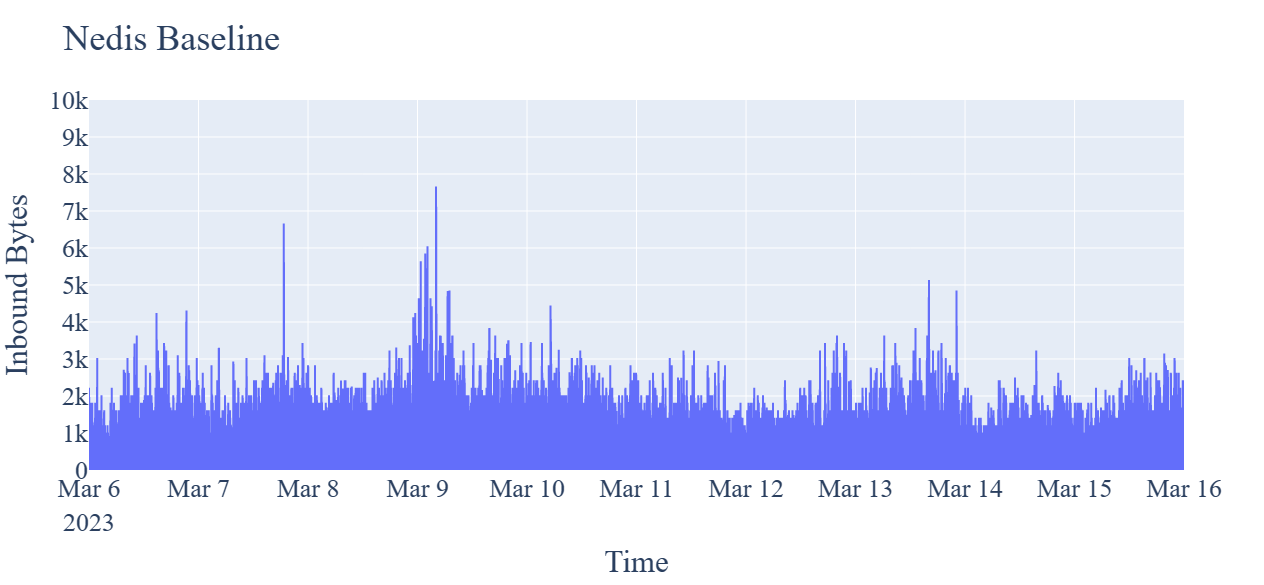
\includegraphics[width=\textwidth]{figures/Nedis_Baseline_InboundBytes.png}
        \caption{Inbound Bytes}
        \label{fig:NedisBaselineInboundBytes}
    \end{subfigure}
    \begin{subfigure}[b]{0.7\textwidth}
        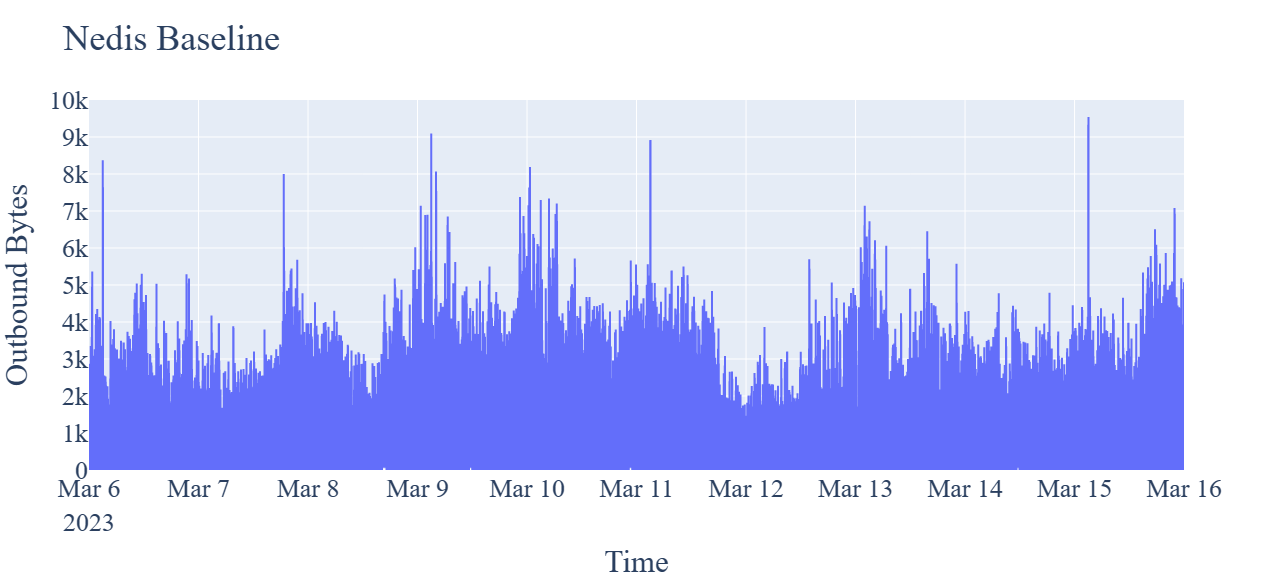
\includegraphics[width=\textwidth]{figures/Nedis_Baseline_OutboundBytes.png}
        \caption{Outbound Bytes}
        \label{fig:NedisBaselineOutboundBytes}
    \end{subfigure}
    \caption{Nedis Baseline Inbound and Outbound Bytes}
    \label{Fig:NedisBaselineOutandInboundBytes}
 \end{figure}

 \begin{figure}[H]
    \centering
    \begin{subfigure}[b]{0.7\textwidth}
        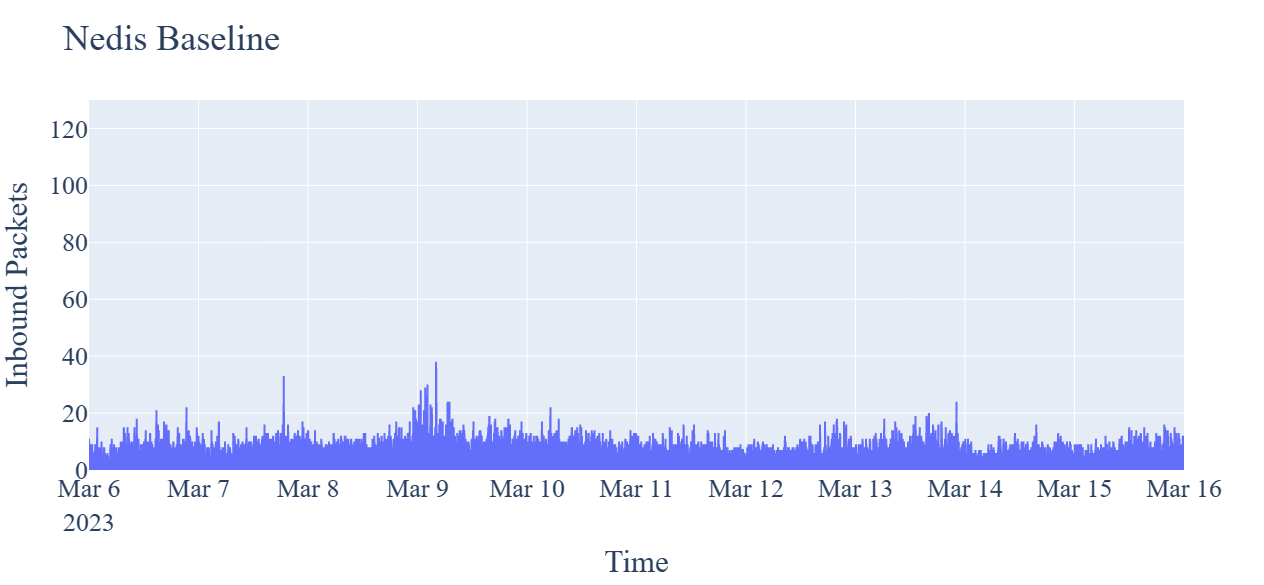
\includegraphics[width=\textwidth]{figures/Nedis_Baseline_InboundPackets.png}
        \caption{Inbound Packets}
        \label{fig:NedisBaselineInboundPackets}
    \end{subfigure}
    \begin{subfigure}[b]{0.7\textwidth}
        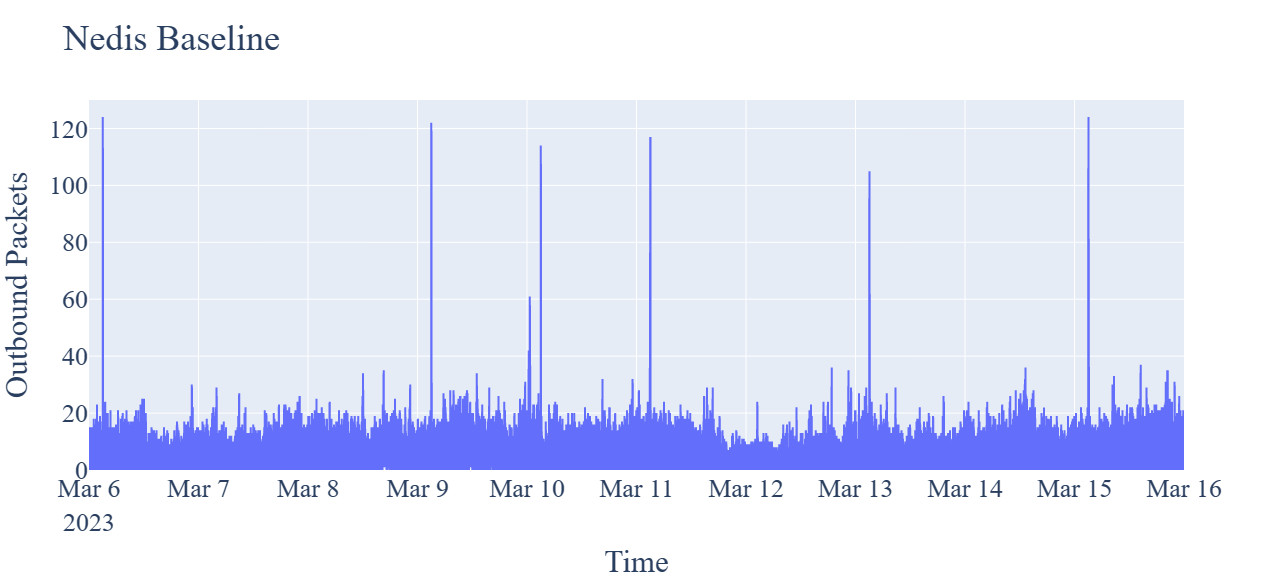
\includegraphics[width=\textwidth]{figures/Nedis_Baseline_OutboundPackets.png}
        \caption{Outbound Packets}
        \label{fig:NedisBaselineOutboundPackets}
    \end{subfigure}
    \caption{Nedis Baseline Inbound and Outbound Packets}
    \label{Fig:NedisBaselineOutandInboundPackets}
 \end{figure}
 
\begin{table}[H]
    \caption{Calculations for Nedis Baseline Capture}
    \centering
    \begin{tabular}{ll|l|}
        \cline{3-3}                                               &                               &             \textbf{Numbers} \\ \hline
        \multicolumn{1}{|c|}{\multirow{4}{*}{\textbf{Total}}}    & Packets              & 2,428,701         \\ \cline{2-3} 
        \multicolumn{1}{|c|}{}                                   & Bytes                & 295,022,494       \\ \cline{2-3} 
        \multicolumn{1}{|c|}{}                                   & Average bytes/second & 341               \\ \cline{2-3} 
        \multicolumn{1}{|c|}{}                                   & Average packet size  & 121 bytes        \\ \hline
        \multicolumn{1}{|l|}{\multirow{5}{*}{\textbf{Inbound}}}  & Packets              & 451,495           \\ \cline{2-3} 
        \multicolumn{1}{|l|}{}                                   & Bytes                & 88,595,049        \\ \cline{2-3} 
        \multicolumn{1}{|l|}{}                                   & Average bytes/second & 102                \\ \cline{2-3} 
        \multicolumn{1}{|l|}{}                                   & Average packet size  & 196 bytes         \\ \cline{2-3} 
        \multicolumn{1}{|l|}{}                                   & Biggest packet       & 522 bytes        \\ \hline
        \multicolumn{1}{|l|}{\multirow{5}{*}{\textbf{Outbound}}} & Packets              & 1,977,206         \\ \cline{2-3} 
        \multicolumn{1}{|l|}{}                                   & Bytes                & 206,427,445      \\ \cline{2-3} 
        \multicolumn{1}{|l|}{}                                   & Average bytes/second & 238               \\ \cline{2-3} 
        \multicolumn{1}{|l|}{}                                   & Average packet size  & 104 bytes         \\ \cline{2-3} 
        \multicolumn{1}{|l|}{}                                   & Biggest packet       & 485 bytes       \\ \hline
    \end{tabular}
    \label{tab:NedisBaselineCalculations}
\end{table} 


\section{Test Case 1: Cooking}
This chapter presents the results and analysis conducted on Test Case 1: Cooking. The first subsection will present general information applicable to all the devices, and the following subsections will present the result and analysis for each of the devices separately. 
\subsection{General}
The cooking events are 10 in total and are presented in Table \ref{tab:CookingDates}. Every device has the same dates for this event. 
\begin{table}[!hbtp]
    \centering
    \caption{Date and time for Test Case 1: Cooking Events}
    \begin{adjustbox}{width=1\textwidth}
            \begin{tabular}{l|l|l|l|l|l|l|l|l|l|l|l|l|l|l|l|}
            \cline{2-16} 
            & 08.01 & 09.01 & 10.01 & 11.01 & 12.01 & 16.01 & 18.01 & 19.01 & 24.01 & 25.01 & 26.01 & 30.01 & 31.01 & 01.02 & 02.02 \\
            \hline
            \multicolumn{1}{|l|}{Started event}  & 15:58 & 15:59 & 16:01 & 16:05 & 16:10 & 16:02 & 16:04 & 16:01 & 15:57 & 16:02 & 16:01 & 16:01 & 16:01 & 16:02 & 16:02 \\ 
            \hline
            \multicolumn{1}{|l|}{Finished event} & 16:22 & 16:21 & 16:27 & 16:37 & 16:28 & 16:25 & 16:25 & 16:18 & 16:20 & 16:13 & 16:25 & 16:19 & 16:21 & 16:22 & 16:22 \\ 
            \hline
            \end{tabular}
    \end{adjustbox}
    \label{tab:CookingDates}
\end{table}
\FloatBarrier

To be able to look even further into differences from when the devices are in an environment when an event is ongoing and when it is in the same environment, but without any event ongoing, graphs and calculations from the baseline traffic are used to compare. To choose a time for the baseline traffic, all start values from the actual events in Table \ref{tab:CookingDates} are used to calculate an average value for starting time. The same applies to end time. Calculated average value for the cooking event is:

\begin{itemize}
    \item Event Start: 15:58
    \item Event Finished: 16:22
\end{itemize}
\newpage

\subsection{Netatmo Home Coach}
The graphs in figure \ref{fig:NetatmoCookingBytes} and \ref{fig:NetatmoCookingPackets} shows both bytes and packets for the first 10 cooking events. The area marked red on the graphs are when the event was ongoing. Table \ref{tab:NetatmoCookingCalculations} presents the calculations from all the cooking events. The table also includes average and standard deviation (std deviation) values for the events. 

\begin{table}[!ht]
    \centering
    \caption{Netatmo Cooking Calculations}
    \begin{tabular}{|l|l|l|l|l|l|}
    \hline
        \textbf{Event dates} & \textbf{Packets} & \textbf{Bytes} & \textbf{Biggest packet} \\ \hline
        08.jan & 789 & 107,094 & 407 bytes \\ \hline
        09.jan & 589 & 81,694 & 407 bytes \\ \hline
        10.jan & 786 & 105,351 & 203 bytes \\ \hline
        11.jan & 791 & 107,011 & 407 bytes \\ \hline
        12.jan & 528 & 71,873 & 407 bytes \\ \hline
        16.jan & 921 & 123,899 & 407 bytes \\ \hline
        18.jan & 739 & 108,857 & 407 bytes  \\ \hline
        19.jan & 607 & 82,423 & 407 bytes \\ \hline
        24.jan & 836 & 114,340 & 407 bytes \\ \hline
        25.jan & 309 & 42,332 & 407 bytes \\ \hline
        26.jan & 739 & 100,223 & 407 bytes \\ \hline
        30.jan & 654 & 89,264 & 407 bytes \\ \hline
        31.jan & 704 & 93,998 & 136 bytes \\ \hline
        01.feb & 644 & 87,474 & 407 bytes \\ \hline
        02.feb & 666 & 91,485 & 407 bytes \\ \hline
        \textbf{Average} &  \textbf{687}  &  \textbf{93,821}  &  \textbf{375 bytes} \\ \hline
        \textbf{Std deviation} &  \textbf{147}  & \textbf{19,914}  &  \textbf{85 bytes} \\ \hline
    \end{tabular}
    \label{tab:NetatmoCookingCalculations}
\end{table}

\begin{figure}[H]
    \centering
    \begin{subfigure}{0.49\textwidth}
       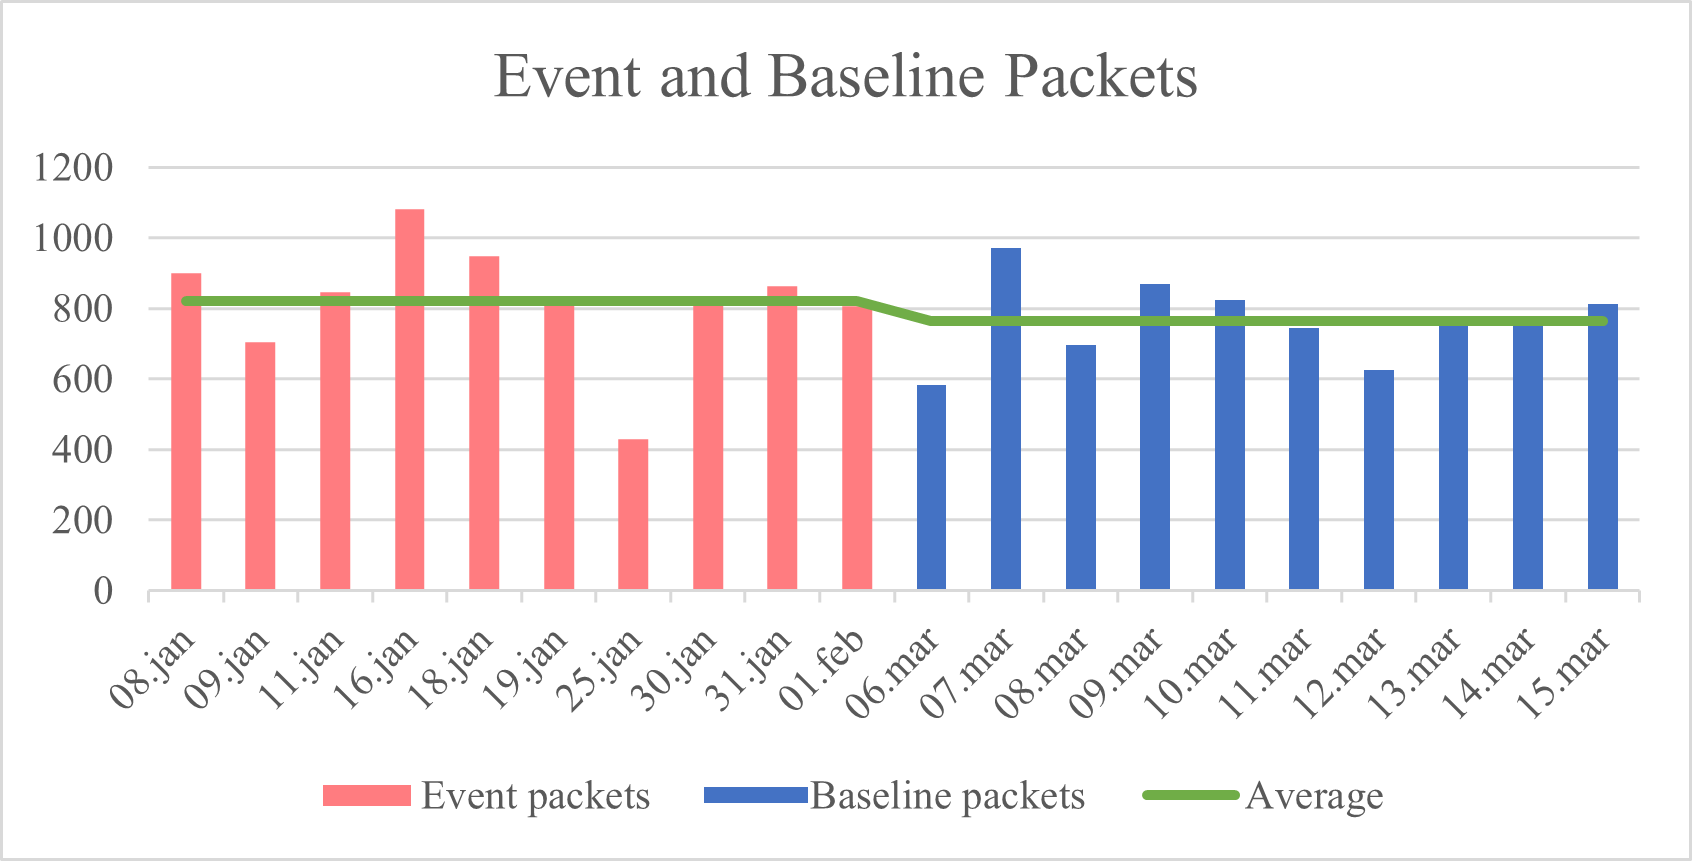
\includegraphics[width=1\hsize]{figures/Netatmo_Cooking_Calculations_Packets.png} 
    \end{subfigure}
    \begin{subfigure}{0.49\textwidth}
        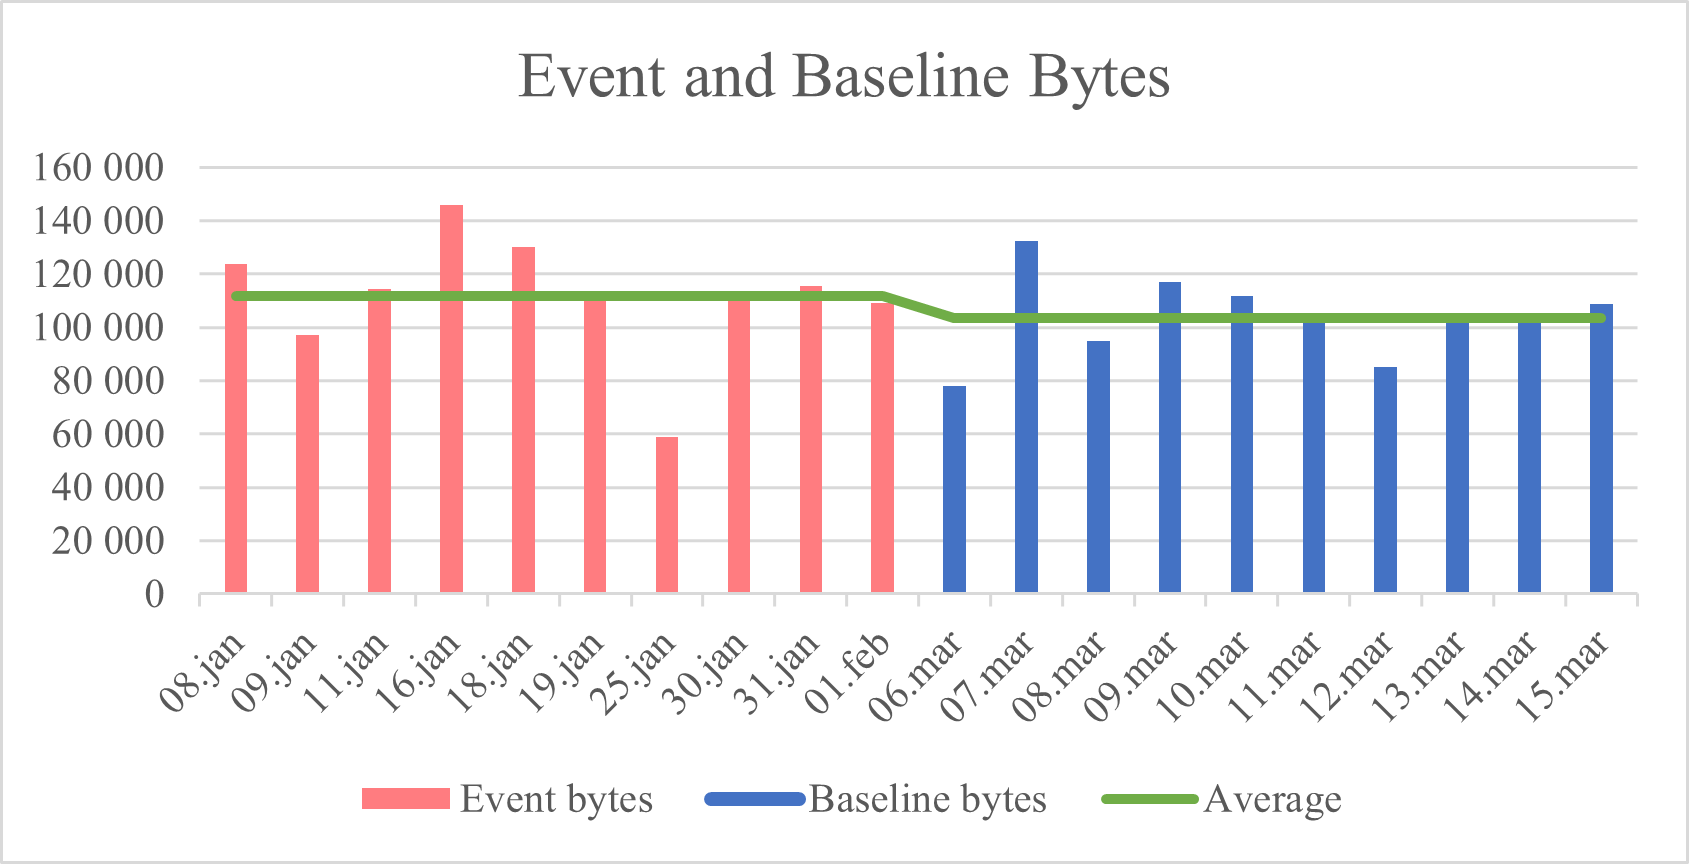
\includegraphics[width=1\hsize]{figures/Netatmo_Cooking_Calculations_Bytes.png} 
    \end{subfigure}
    \caption{Netatmo Cooking Calculations with Packets and Bytes}
    \label{fig:NetatmoCookingCalculations}
\end{figure}

\begin{figure}[H]
    \begin{subfigure}[b]{0.47\textwidth}
        \centering
        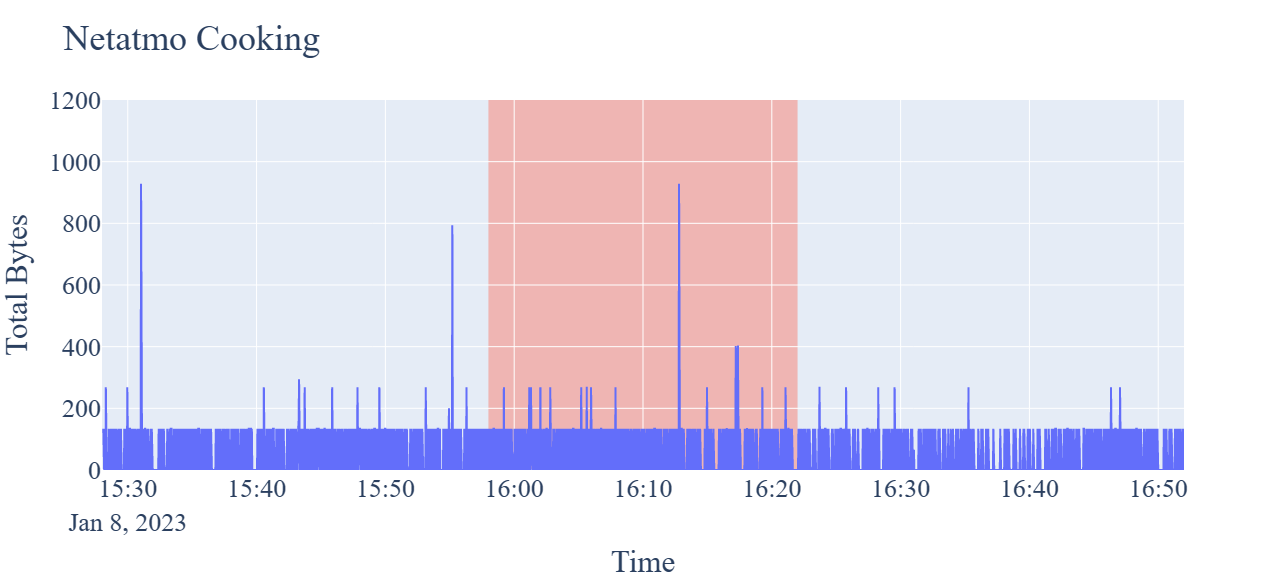
\includegraphics[width=1.2\hsize]{figures/Netatmo_Cooking_Bytes_08.01.png}
    \end{subfigure}
    \begin{subfigure}[b]{0.47\textwidth}
        \centering
        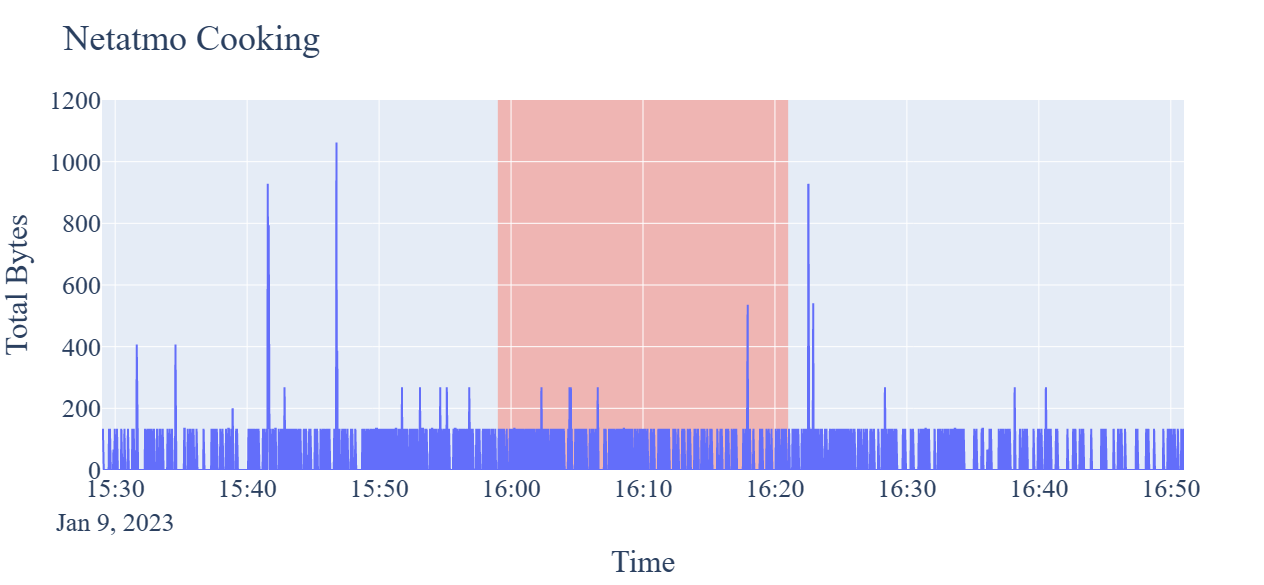
\includegraphics[width=1.2\hsize]{figures/Netatmo_Cooking_Bytes_09.01.png}
    \end{subfigure}
    \begin{subfigure}[b]{0.47\textwidth}
        \centering
        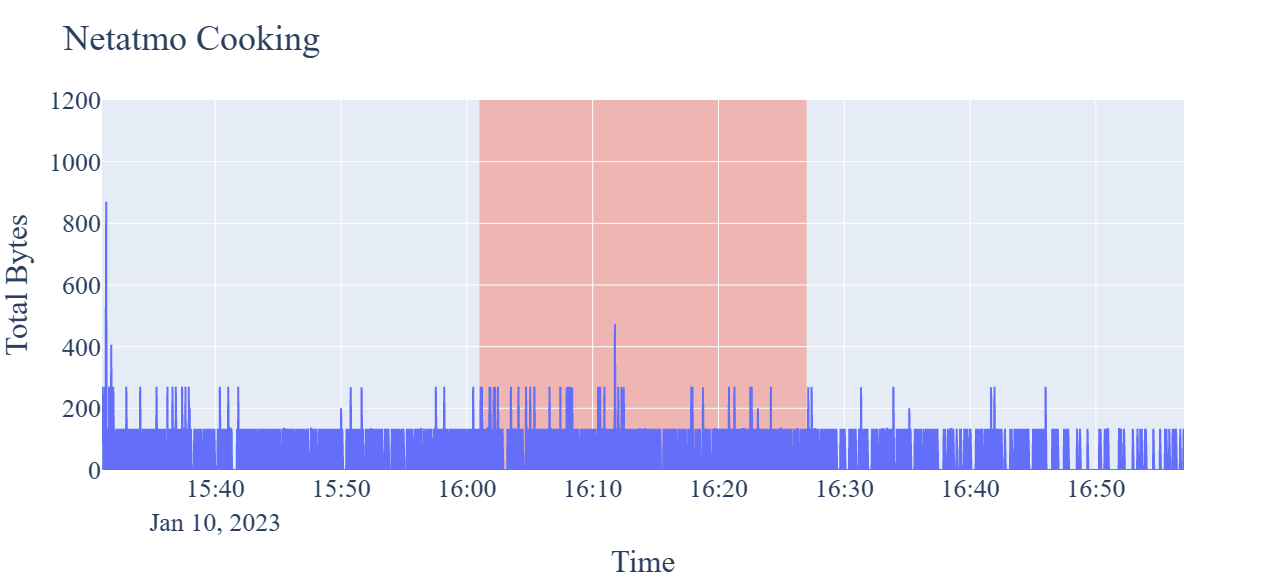
\includegraphics[width=1.2\hsize]{figures/Netatmo_Cooking_Bytes_10.01.png}
    \end{subfigure}
    \begin{subfigure}[b]{0.47\textwidth}
        \centering
        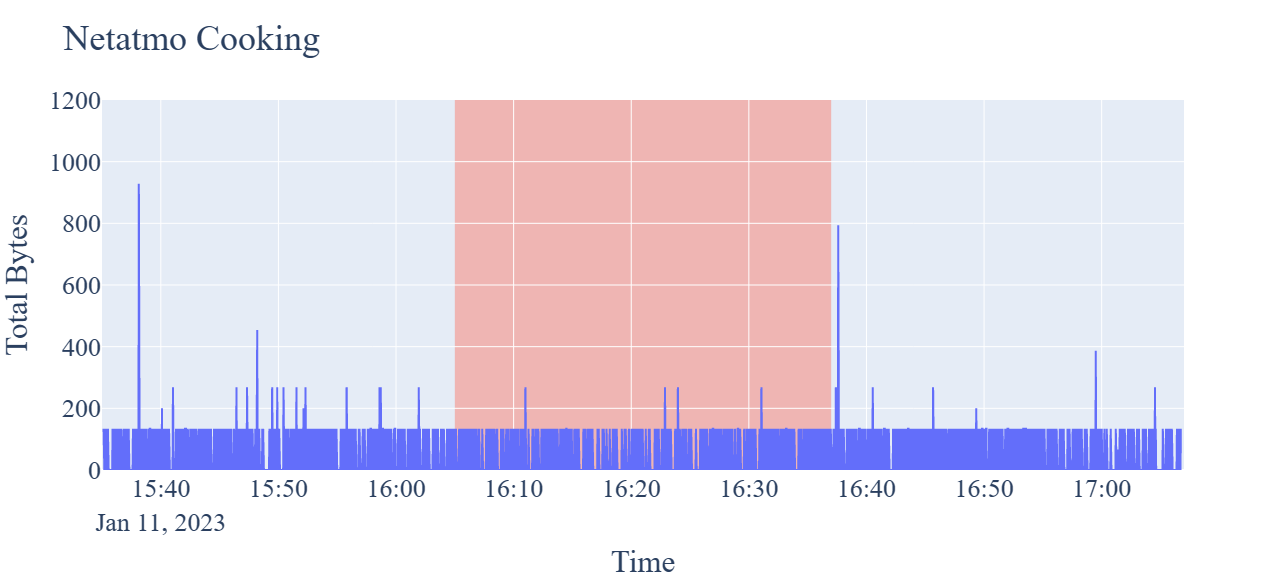
\includegraphics[width=1.2\hsize]{figures/Netatmo_Cooking_Bytes_11.01.png}
    \end{subfigure}
    \begin{subfigure}[b]{0.47\textwidth}
        \centering
        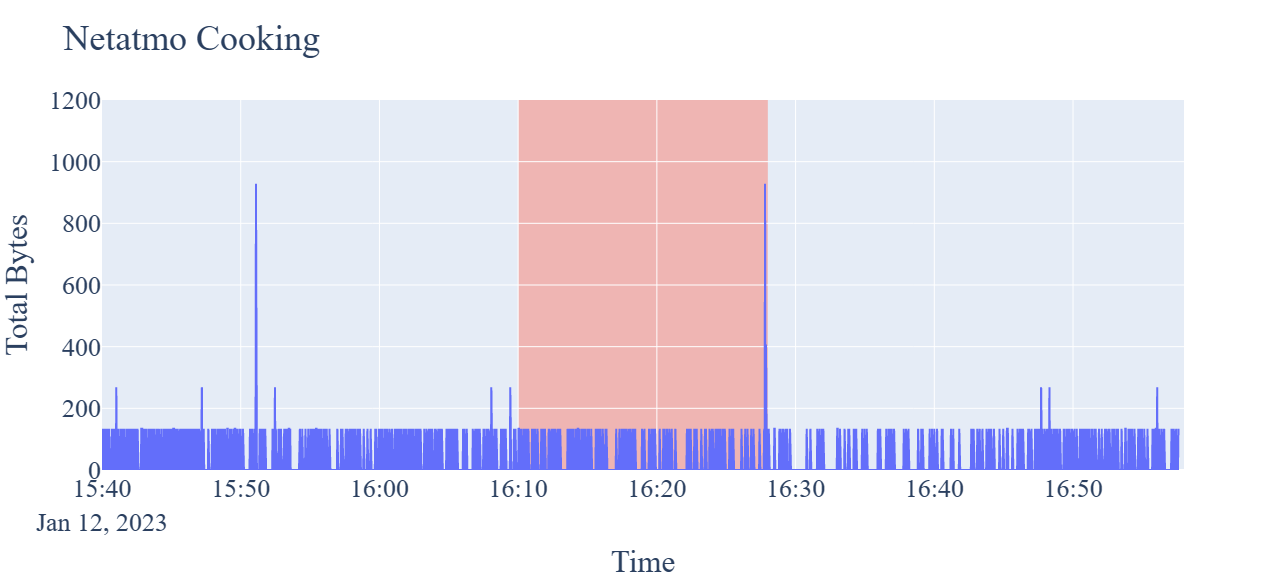
\includegraphics[width=1.2\hsize]{figures/Netatmo_Cooking_Bytes_12.01.png}
    \end{subfigure}
    \begin{subfigure}[b]{0.47\textwidth}
        \centering
        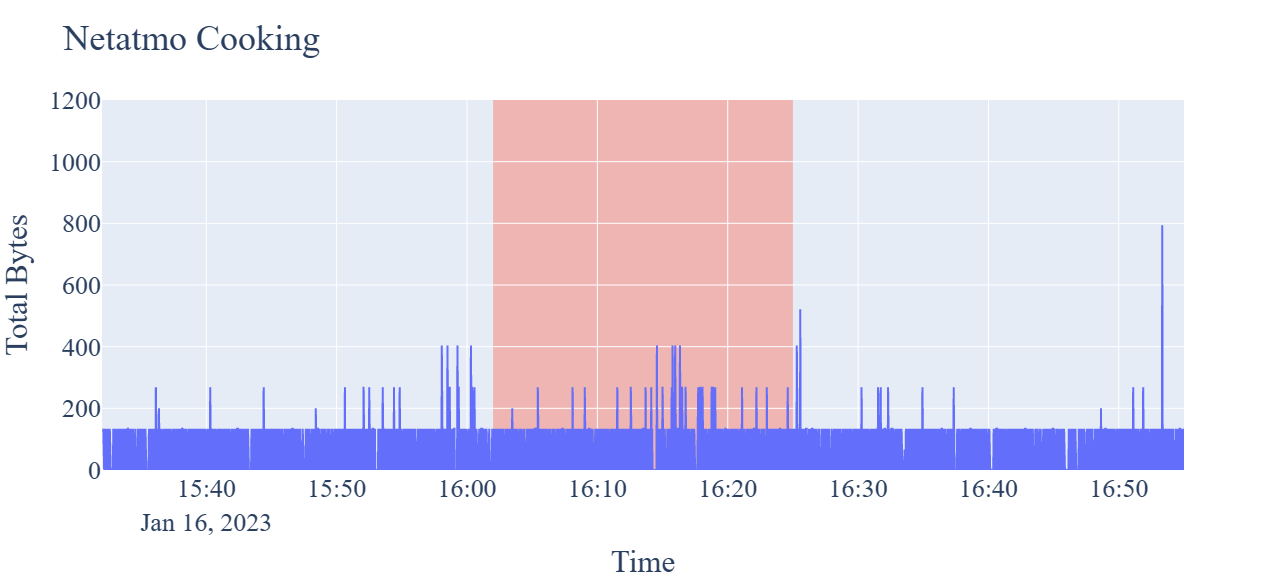
\includegraphics[width=1.2\hsize]{figures/Netatmo_Cooking_Bytes_16.01.png}
    \end{subfigure}
    \begin{subfigure}[b]{0.47\textwidth}
        \centering
        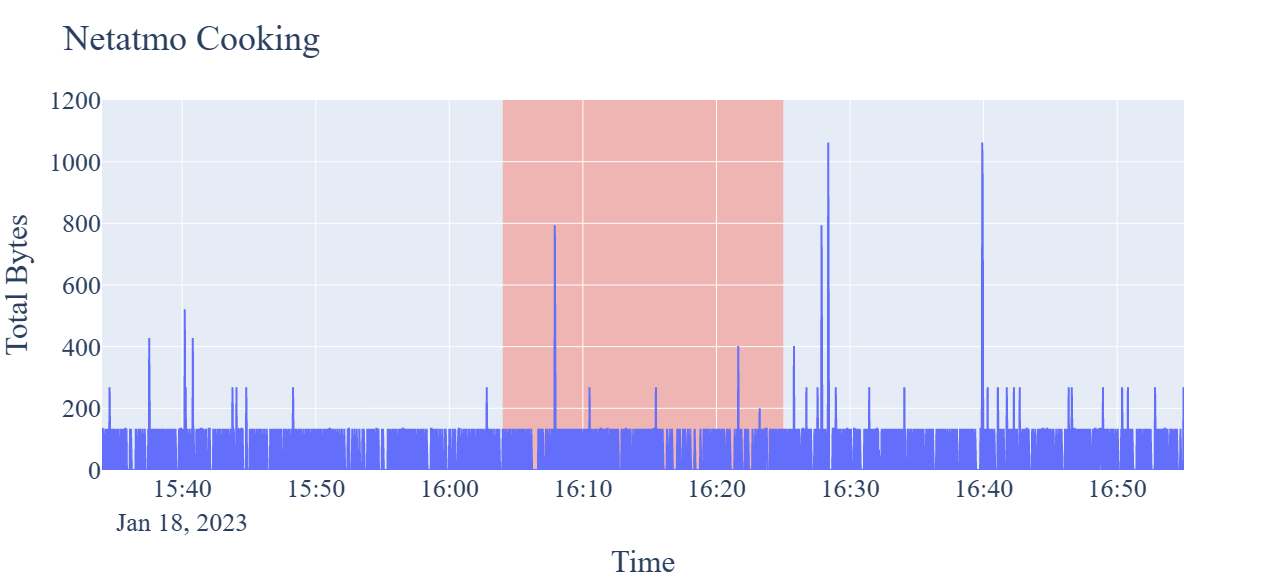
\includegraphics[width=1.2\hsize]{figures/Netatmo_Cooking_Bytes_18.01.png}
    \end{subfigure}
    \begin{subfigure}[b]{0.47\textwidth}
        \centering
        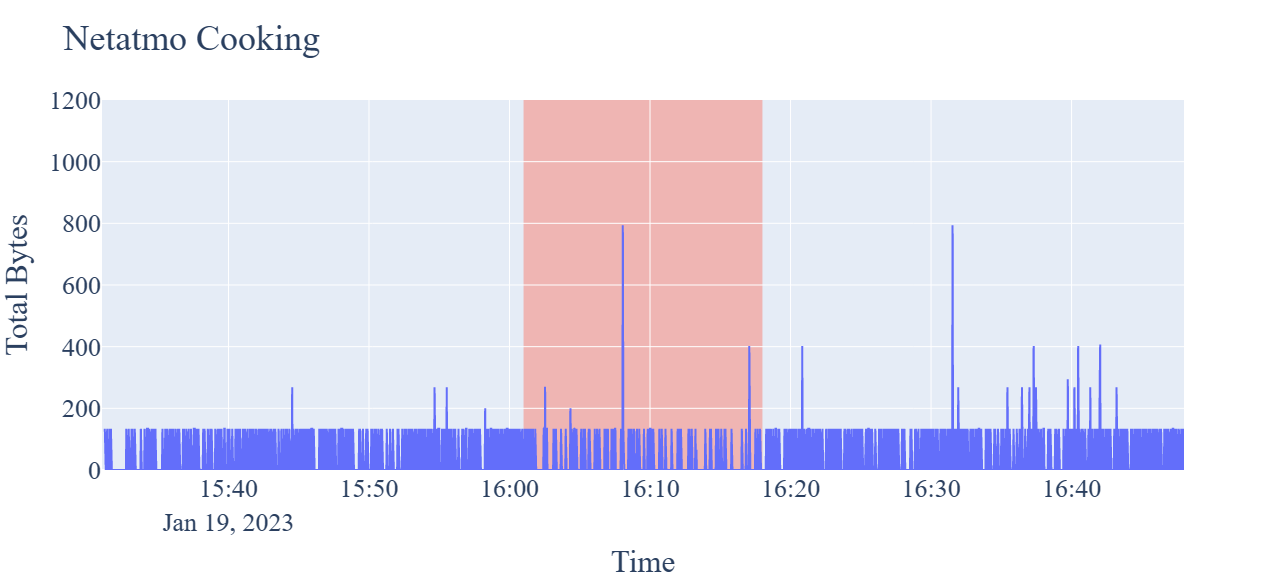
\includegraphics[width=1.2\hsize]{figures/Netatmo_Cooking_Bytes_19.01.png}
    \end{subfigure}
    \begin{subfigure}[b]{0.47\textwidth}
        \centering
        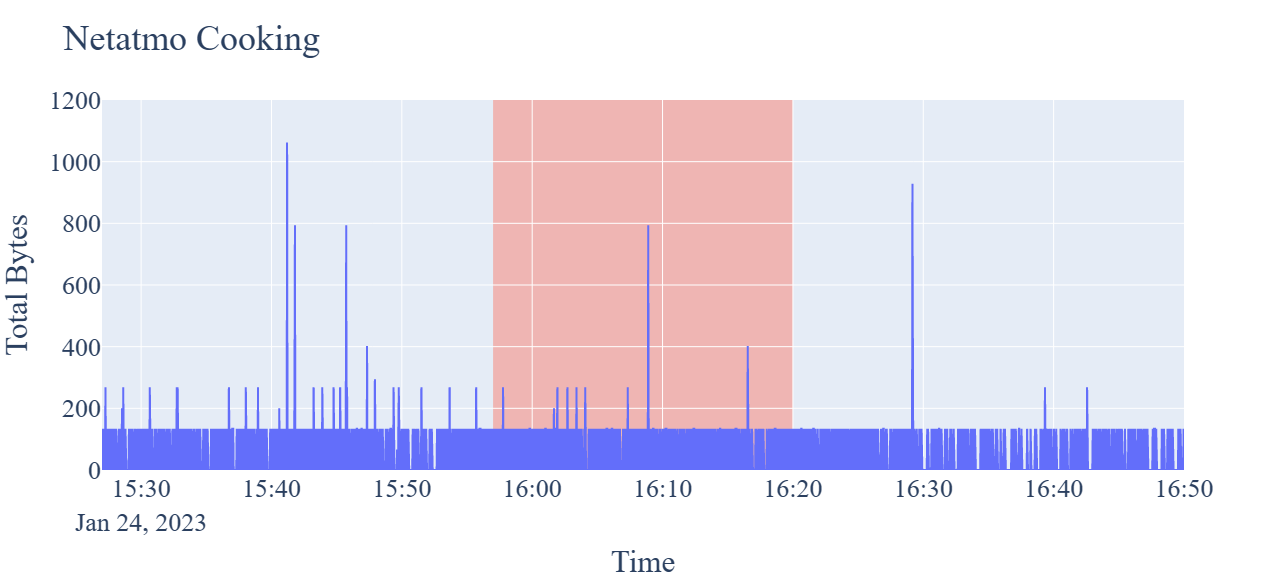
\includegraphics[width=1.2\hsize]{figures/Netatmo_Cooking_Bytes_24.01.png}
    \end{subfigure}
    \begin{subfigure}[b]{0.47\textwidth}
        \centering
        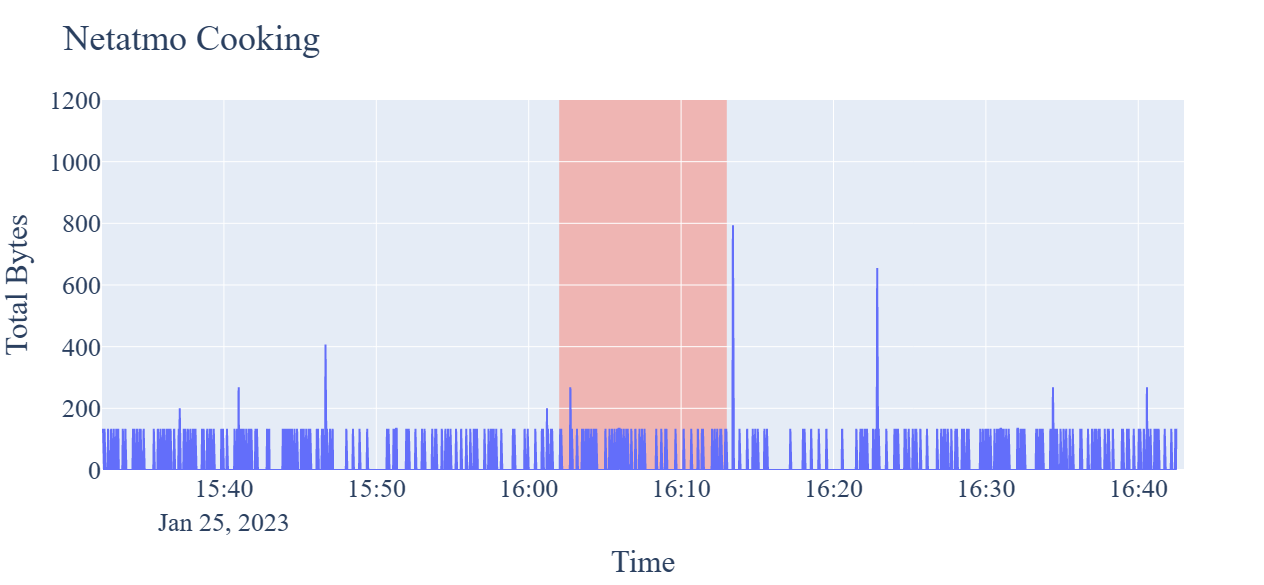
\includegraphics[width=1.2\hsize]{figures/Netatmo_Cooking_Bytes_25.01.png}
    \end{subfigure}
    \begin{subfigure}[b]{0.47\textwidth}
        \centering
        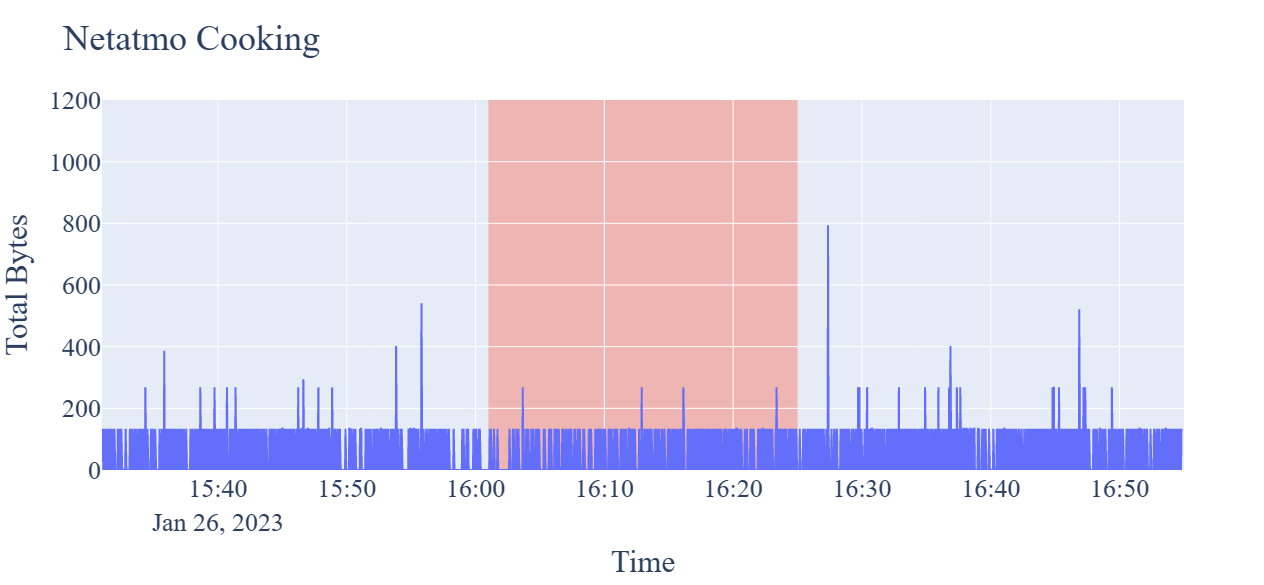
\includegraphics[width=1.2\hsize]{figures/Netatmo_Cooking_Bytes_26.01.png}
    \end{subfigure}
    \hspace{0.6cm}
    \begin{subfigure}[b]{0.47\textwidth}
        \centering
        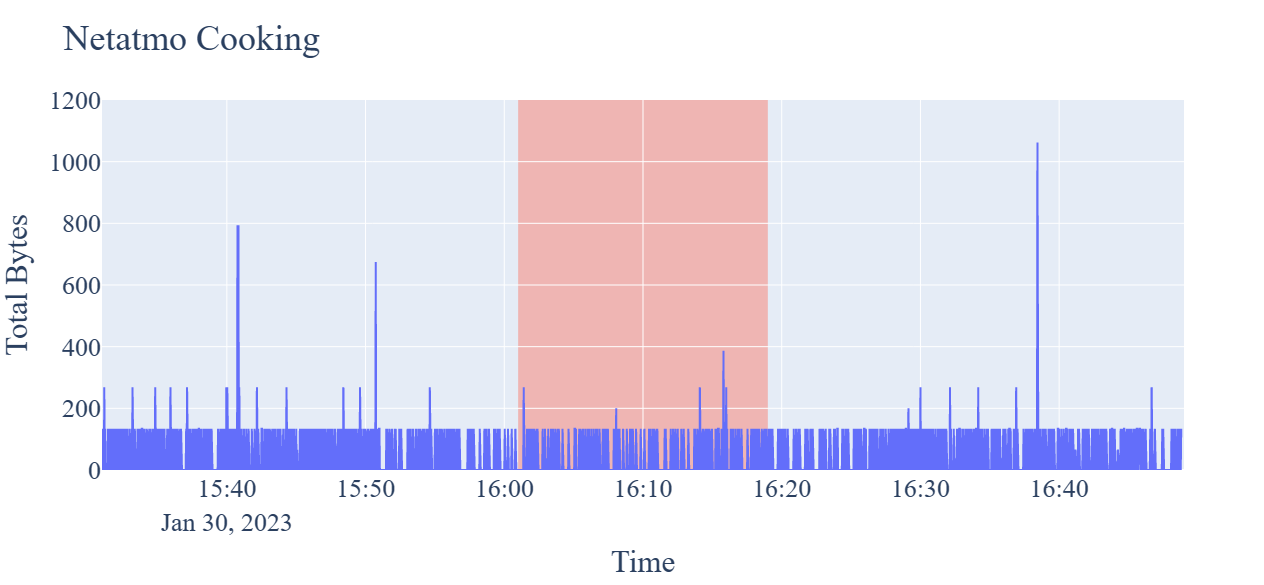
\includegraphics[width=1.2\hsize]{figures/Netatmo_Cooking_Bytes_30.01.png}
    \end{subfigure}
    \caption{Netatmo Cooking Events - Bytes}
    \label{fig:NetatmoCookingBytes}
\end{figure}

\begin{figure}[H]
    \begin{subfigure}[b]{0.47\textwidth}
        \centering
        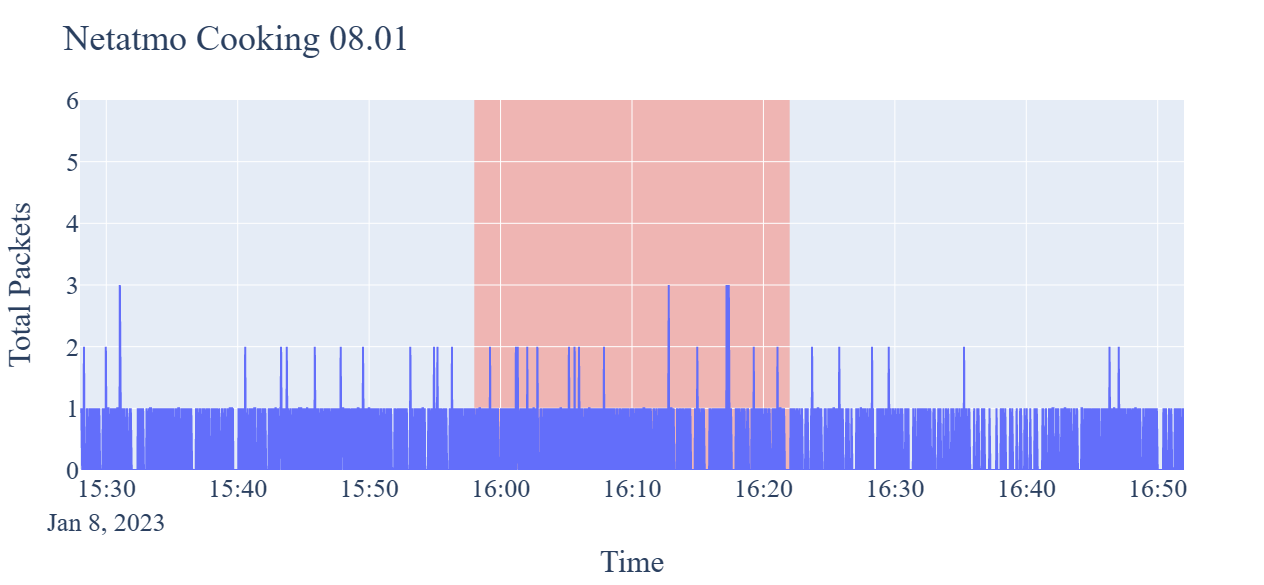
\includegraphics[width=1.2\hsize]{figures/Netatmo_Cooking_Packets_08.01.png}
    \end{subfigure}
    \begin{subfigure}[b]{0.47\textwidth}
        \centering
        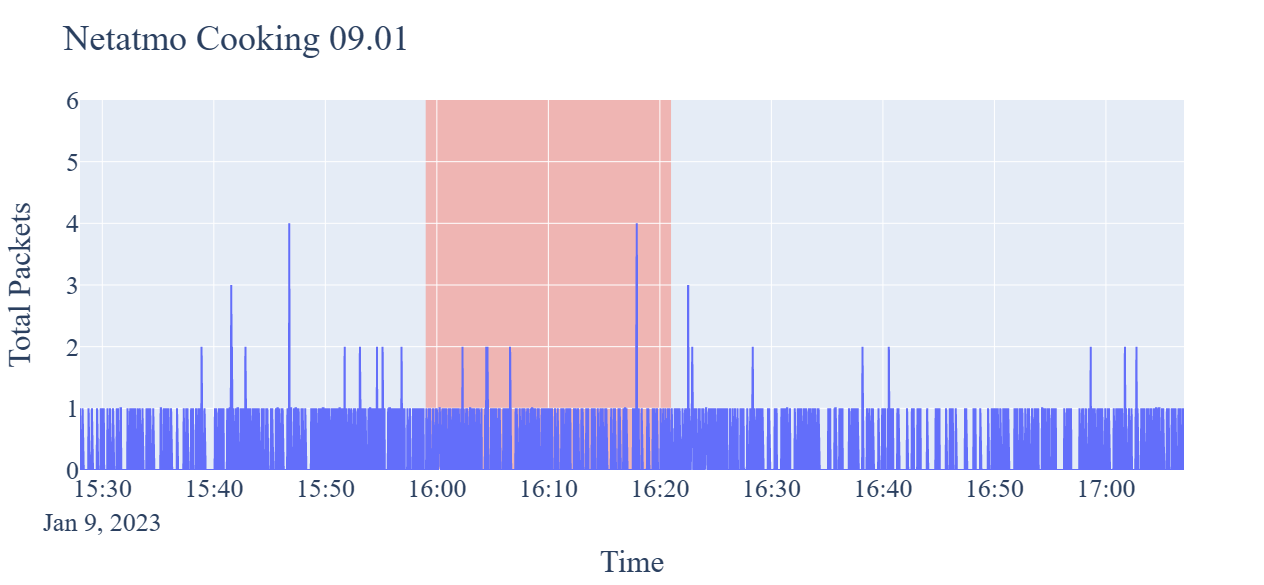
\includegraphics[width=1.2\hsize]{figures/Netatmo_Cooking_Packets_09.01.png}
    \end{subfigure}
    \begin{subfigure}[b]{0.47\textwidth}
        \centering
        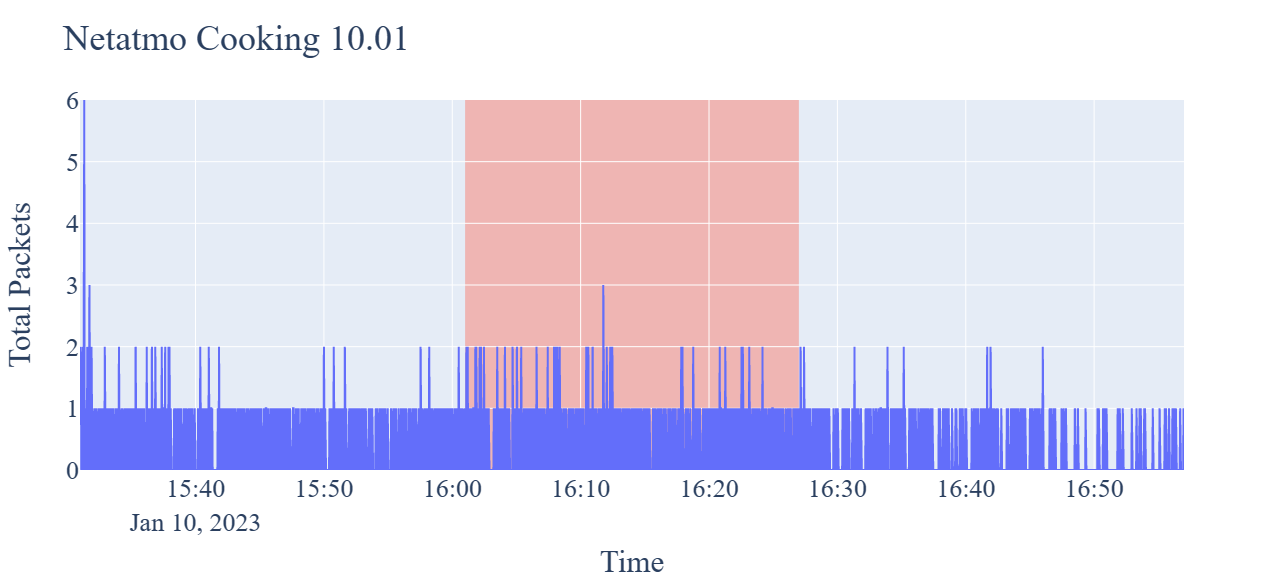
\includegraphics[width=1.2\hsize]{figures/Netatmo_Cooking_Packets_10.01.png}
    \end{subfigure}
    \begin{subfigure}[b]{0.47\textwidth}
        \centering
        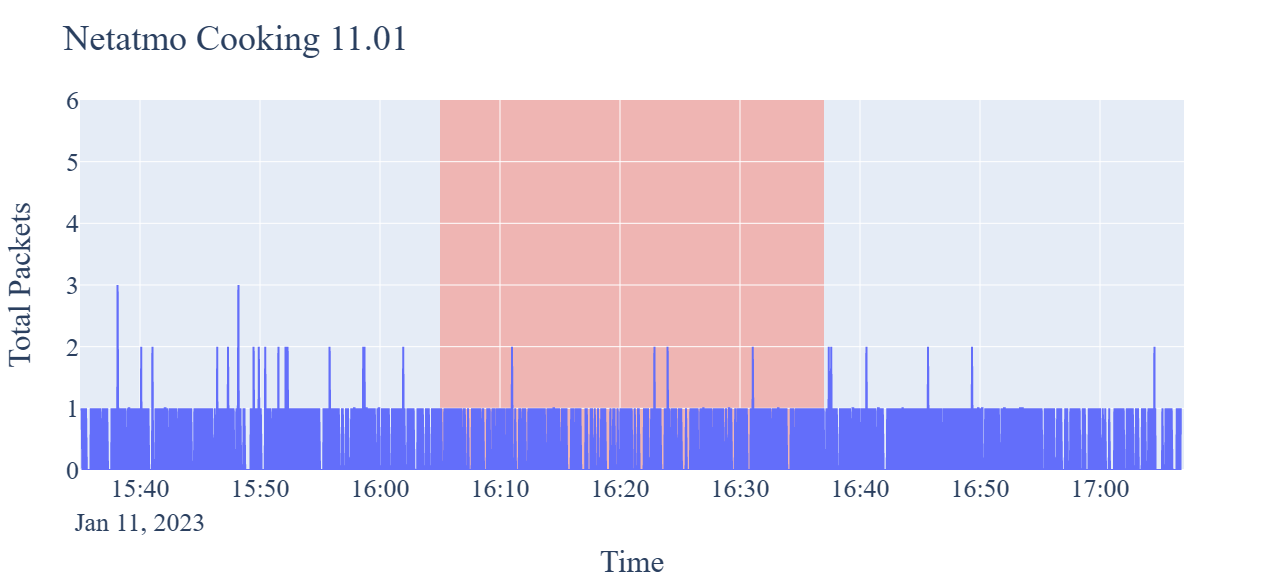
\includegraphics[width=1.2\hsize]{figures/Netatmo_Cooking_Packets_11.01.png}
    \end{subfigure}
    \begin{subfigure}[b]{0.47\textwidth}
        \centering
        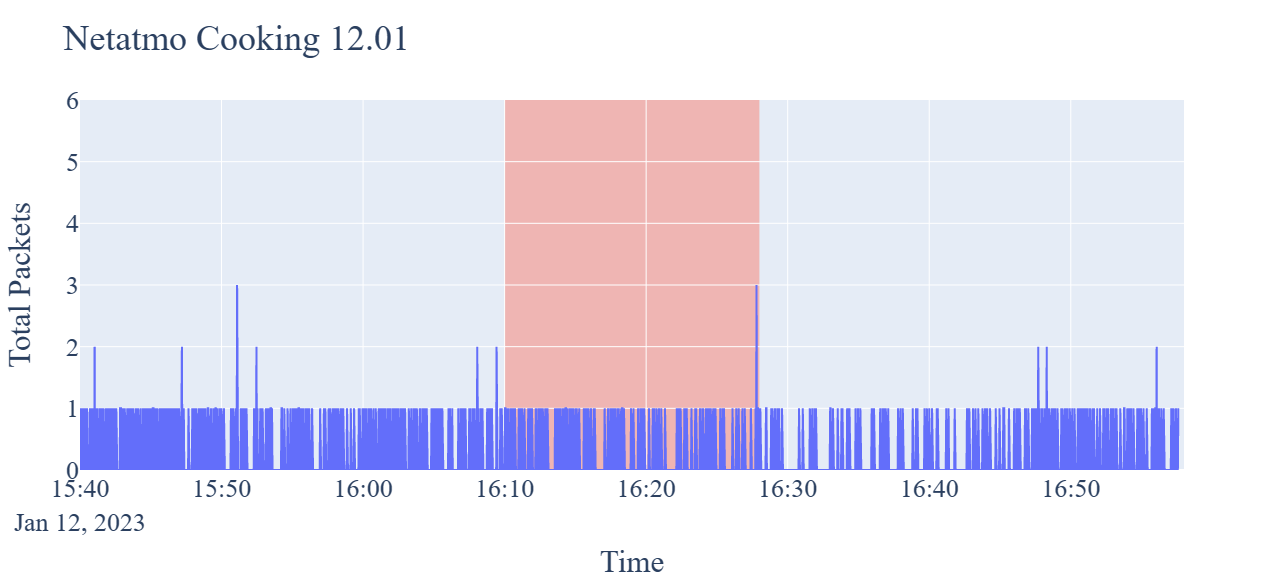
\includegraphics[width=1.2\hsize]{figures/Netatmo_Cooking_Packets_12.01.png}
    \end{subfigure}
    \begin{subfigure}[b]{0.47\textwidth}
        \centering
        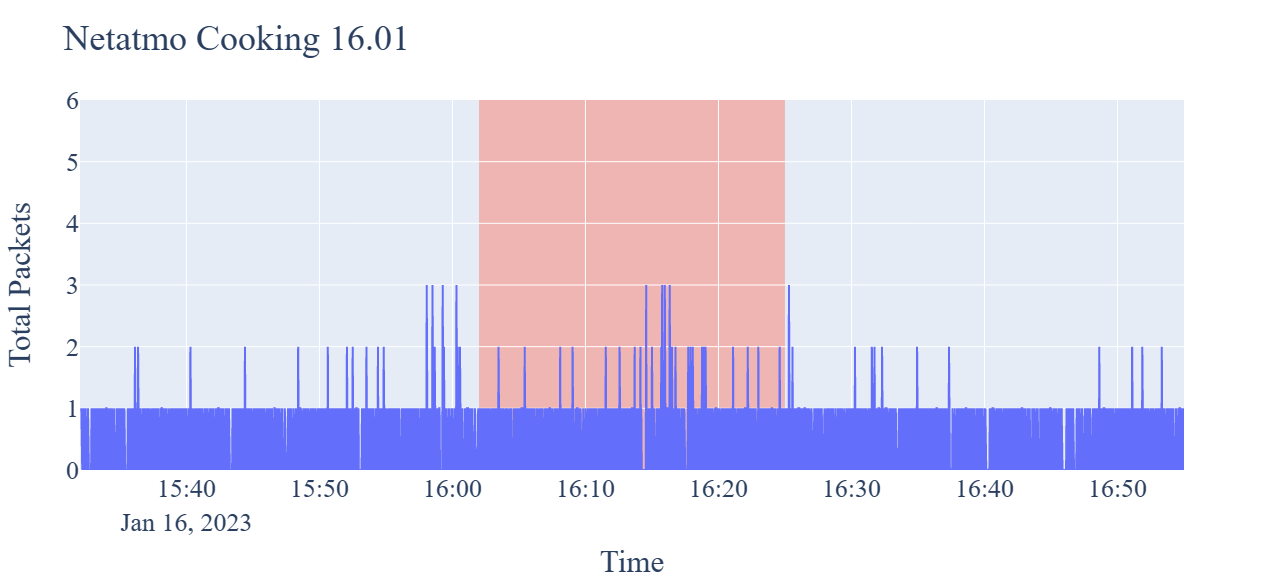
\includegraphics[width=1.2\hsize]{figures/Netatmo_Cooking_Packets_16.01.png}
    \end{subfigure}
    \begin{subfigure}[b]{0.47\textwidth}
        \centering
        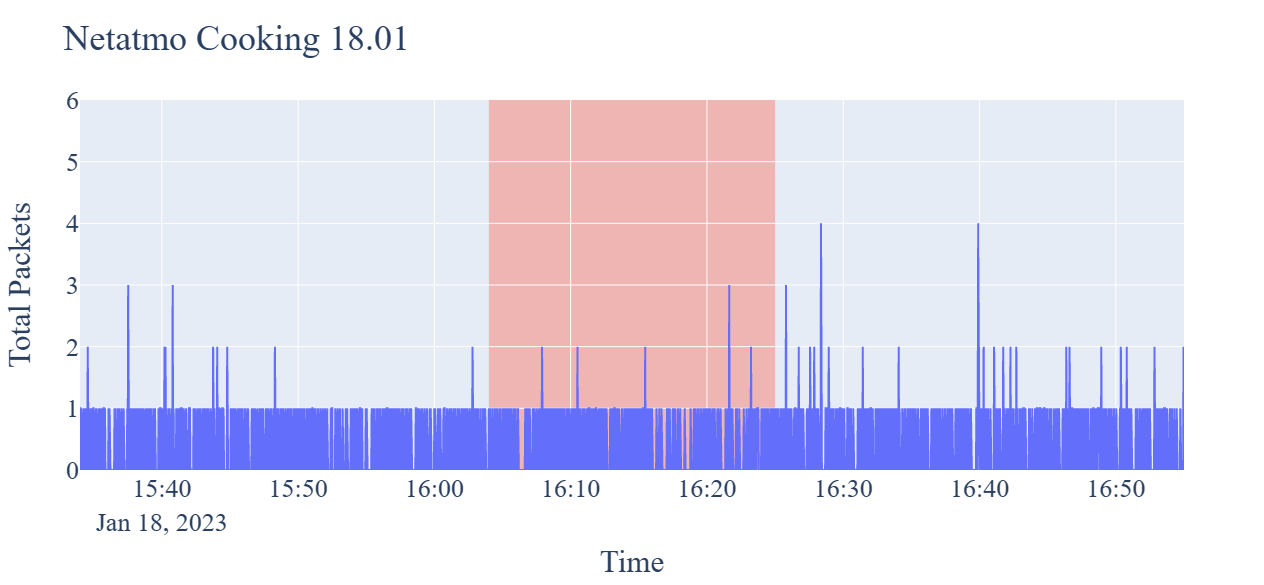
\includegraphics[width=1.2\hsize]{figures/Netatmo_Cooking_Packets_18.01.png}
    \end{subfigure}
    \begin{subfigure}[b]{0.47\textwidth}
        \centering
        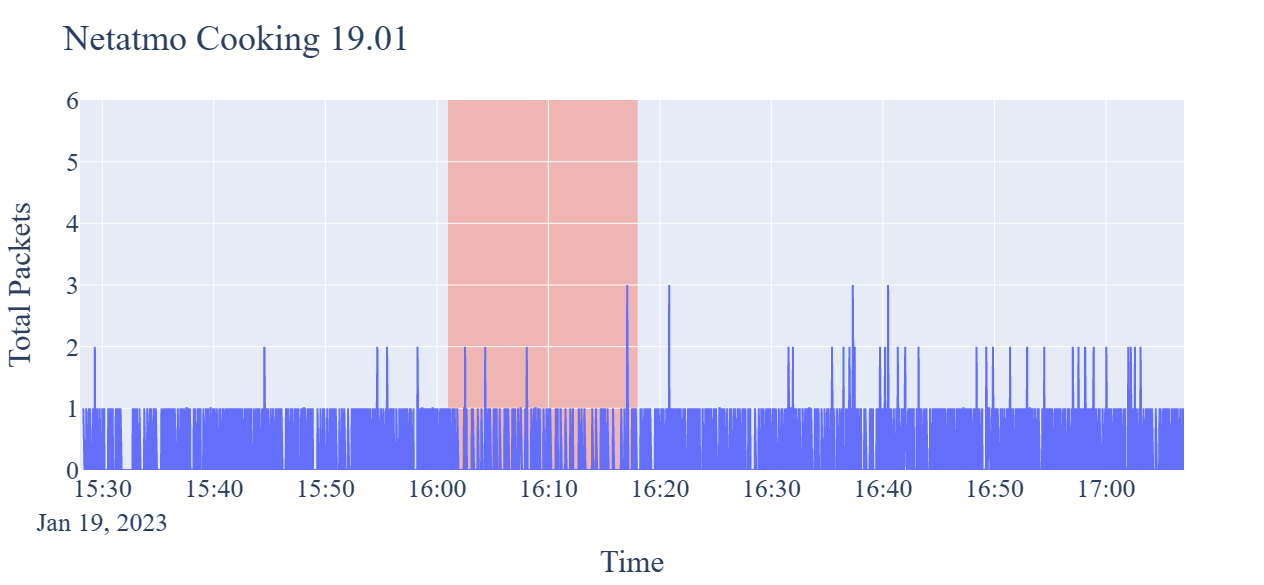
\includegraphics[width=1.2\hsize]{figures/Netatmo_Cooking_Packets_19.01.png}
    \end{subfigure}
    \begin{subfigure}[b]{0.47\textwidth}
        \centering
        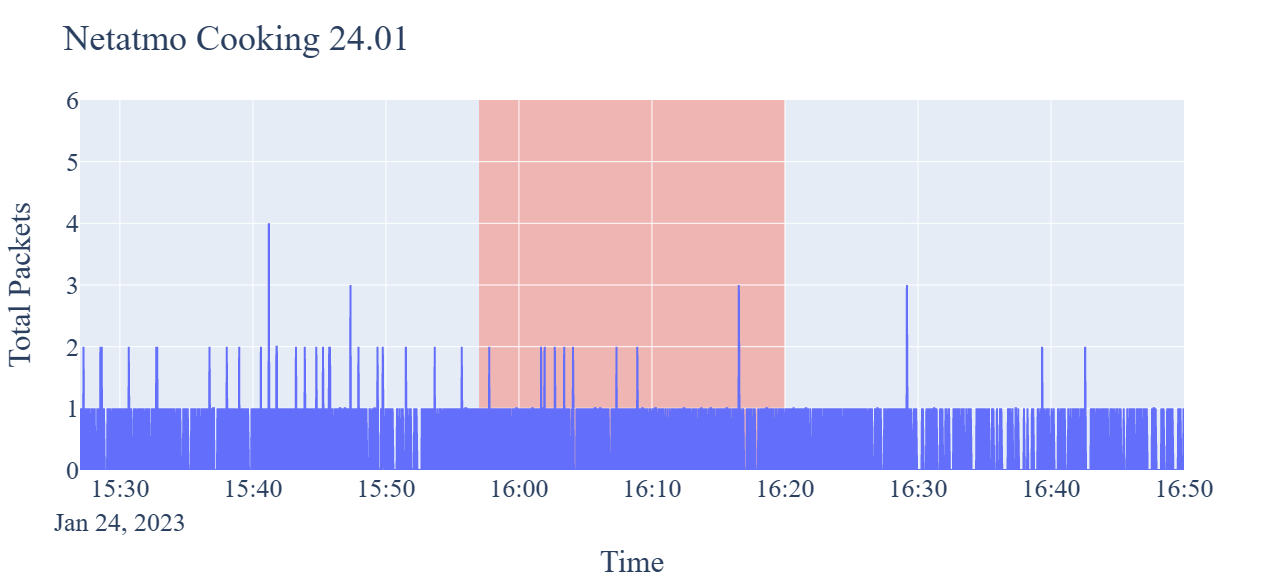
\includegraphics[width=1.2\hsize]{figures/Netatmo_Cooking_Packets_24.01.png}
    \end{subfigure}
    \begin{subfigure}[b]{0.47\textwidth}
        \centering
        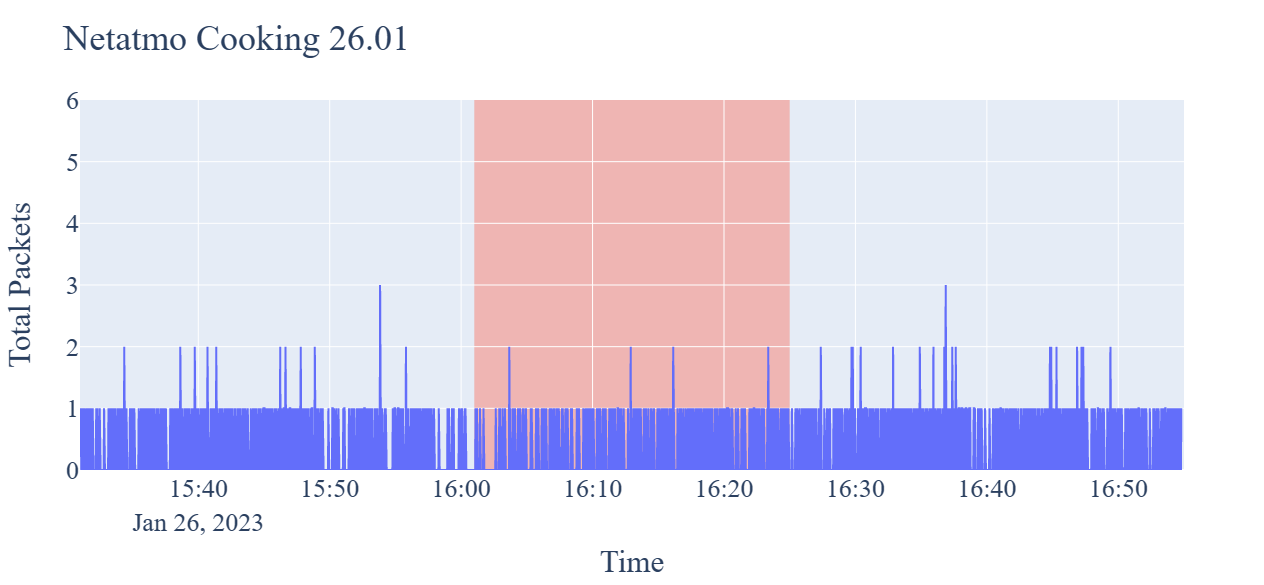
\includegraphics[width=1.2\hsize]{figures/Netatmo_Cooking_Packets_26.01.png}
    \end{subfigure}
    \begin{subfigure}[b]{0.47\textwidth}
        \centering
        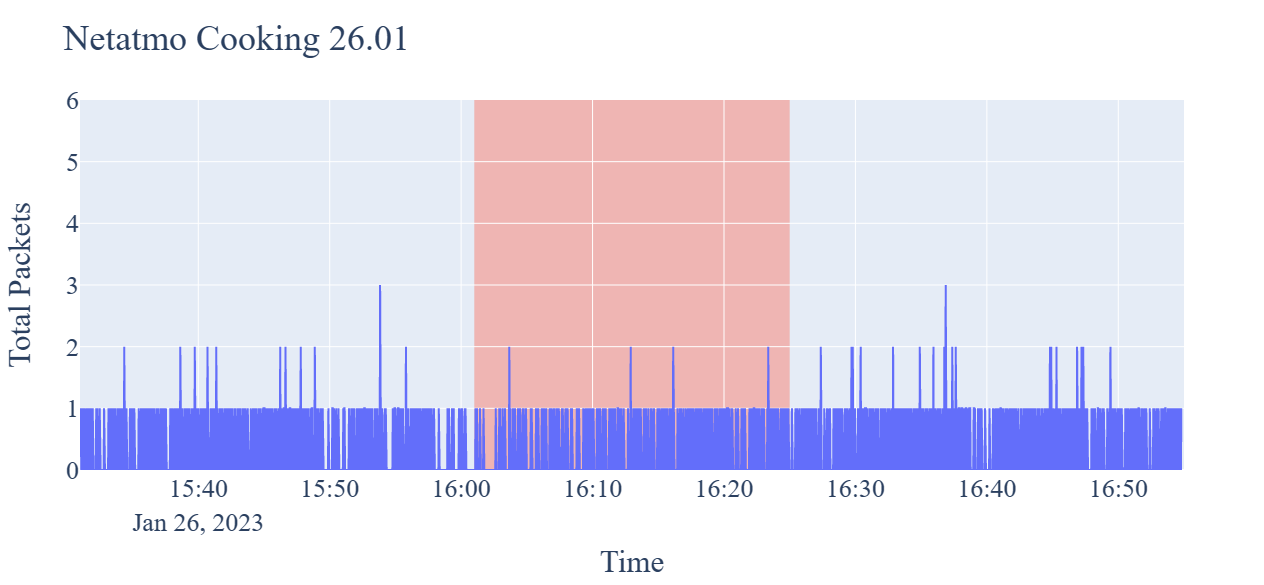
\includegraphics[width=1.2\hsize]{figures/Netatmo_Cooking_Packets_26.01.png}
    \end{subfigure}
    \hspace{0.6cm}
    \begin{subfigure}[b]{0.47\textwidth}
        \centering
        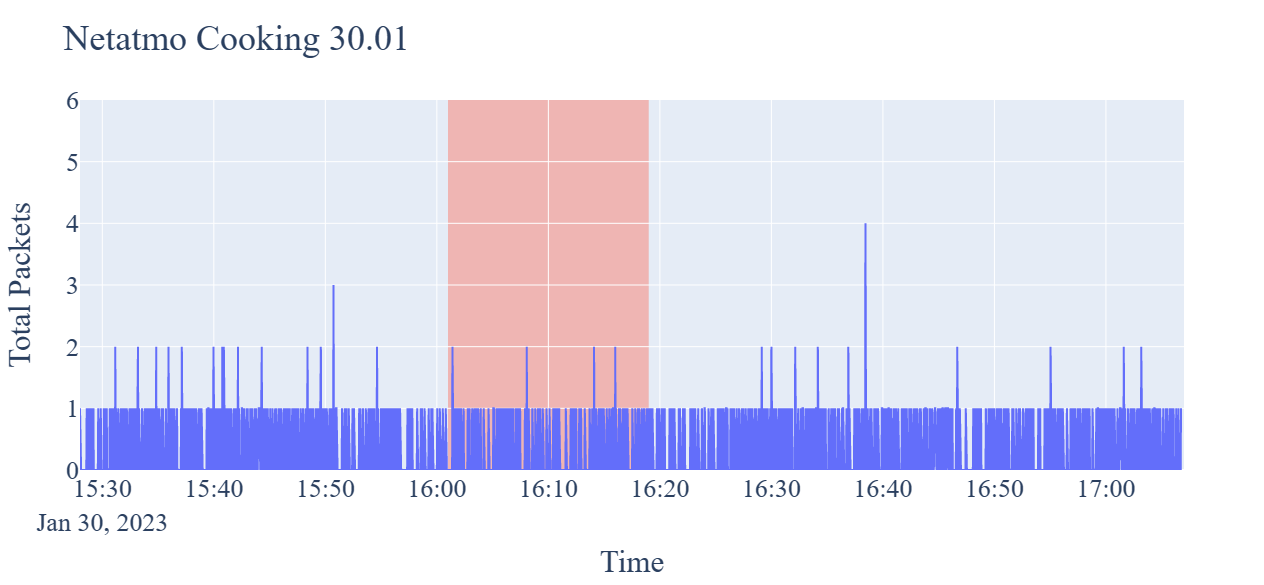
\includegraphics[width=1.2\hsize]{figures/Netatmo_Cooking_Packets_30.01.png}
    \end{subfigure}
    \caption{Netatmo Cooking Events - Packets}
    \label{fig:NetatmoCookingPackets}
\end{figure}

It is hard to see any specific changes in the traffic flow from when the event is ongoing based on the graphs given in figure \ref{fig:NetatmoCookingBytes} and \ref{fig:NetatmoCookingPackets}. Also looking at the table \ref{tab:NetatmoCookingCalculations} the calculations varies a lot. From table \ref{tab:NetatmoCookingCalculations}, the packets varies from 309 to 921 packets and from 42,332 to 123,899 bytes. The biggest packet from the capture is mainly 407 bytes, but for two of the events a 407 byte packet is not sent. When looking at the graphs in figure \ref{fig:NetatmoCookingCalculations}, packets and bytes for each event are compared to each other and the average value. They easier show the differences in the amount of packets captured during the events. 
\\\\
The next step is to compare the event graphs and calculations with the baseline traffic from the correlating timing for cooking events. Figure \ref{fig:NetatmoCookingComparingBytes} and \ref{fig:NetatmoCookingComparingPackets} compares the graphs for cooking from the actual events, marked in red, to the baseline capture, marked in blue. 

\begin{figure}[H]
    \begin{subfigure}[b]{0.47\textwidth}
        \centering
        \tcbincludegraphics[size=fbox,width=1.1\hsize,colframe=red]{figures/Netatmo_Cooking_Packets_08.01.png}
    \end{subfigure}
    \begin{subfigure}[b]{0.47\textwidth}
        \centering
        \tcbincludegraphics[size=fbox,width=1.1\hsize, colframe=blue]{figures/Netatmo_Cooking_Baseline_Packets_06.03.png}
    \end{subfigure}
    \begin{subfigure}[b]{0.47\textwidth}
        \centering
        \tcbincludegraphics[size=fbox,width=1.1\hsize,colframe=red]{figures/Netatmo_Cooking_Packets_10.01.png}
    \end{subfigure}
    \begin{subfigure}[b]{0.47\textwidth}
        \centering
        \tcbincludegraphics[size=fbox,width=1.1\hsize,colframe=blue]{figures/Netatmo_Cooking_Baseline_Packets_07.03.png}
    \end{subfigure}
    \begin{subfigure}[b]{0.47\textwidth}
        \centering
        \tcbincludegraphics[size=fbox,width=1.1\hsize,colframe=red]{figures/Netatmo_Cooking_Packets_12.01.png}
    \end{subfigure}
    \begin{subfigure}[b]{0.47\textwidth}
        \centering
        \tcbincludegraphics[size=fbox,width=1.1\hsize,colframe=blue]{figures/Netatmo_Cooking_Baseline_Packets_08.03.png}
    \end{subfigure}
    \begin{subfigure}[b]{0.47\textwidth}
        \centering
        \tcbincludegraphics[size=fbox,width=1.1\hsize,colframe=red]{figures/Netatmo_Cooking_Packets_18.01.png}
    \end{subfigure}
    \begin{subfigure}[b]{0.47\textwidth}
        \centering
        \tcbincludegraphics[size=fbox,width=1.1\hsize,colframe=blue]{figures/Netatmo_Cooking_Baseline_Packets_09.03.png}
    \end{subfigure}
    \begin{subfigure}[b]{0.47\textwidth}
        \centering
        \tcbincludegraphics[size=fbox,width=1.1\hsize,colframe=red]{figures/Netatmo_Cooking_Packets_24.01.png}
    \end{subfigure}
    \begin{subfigure}[b]{0.47\textwidth}
        \centering
        \tcbincludegraphics[size=fbox,width=1.1\hsize,colframe=blue]{figures/Netatmo_Cooking_Baseline_Packets_10.03.png}
    \end{subfigure}
        \begin{subfigure}[b]{0.47\textwidth}
        \centering
        \tcbincludegraphics[size=fbox,width=1.1\hsize,colframe=red]{figures/Netatmo_Cooking_Packets_26.01.png}
    \end{subfigure}
    \begin{subfigure}[b]{0.47\textwidth}
        \centering
        \tcbincludegraphics[size=fbox,width=1.1\hsize,colframe=blue]{figures/Netatmo_Cooking_Baseline_Packets_11.03.png}
    \end{subfigure}
    \begin{subfigure}[b]{0.47\textwidth}
        \centering
        \tcbincludegraphics[size=fbox,width=1.1\hsize,colframe=red]{figures/Netatmo_Cooking_Packets_30.01.png}
    \end{subfigure}
    \hspace{0.6cm}
    \begin{subfigure}[b]{0.47\textwidth}
    \centering
        \tcbincludegraphics[size=fbox,width=1.1\hsize,colframe=blue]{figures/Netatmo_Cooking_Baseline_Packets_12.03.png}
        \end{subfigure}
    \caption{Comparing Events and Baseline Packets for Cooking - Netatmo}
    \label{fig:NetatmoCookingComparingPackets}
\end{figure}

\begin{figure}[H]
    \begin{subfigure}[b]{0.47\textwidth}
        \centering
        \tcbincludegraphics[size=fbox,width=1.1\hsize,colframe=red]{figures/Netatmo_Cooking_Bytes_08.01.png}
    \end{subfigure}
    \begin{subfigure}[b]{0.47\textwidth}
        \centering
        \tcbincludegraphics[size=fbox,width=1.1\hsize,colframe=blue]{figures/Netatmo_Cooking_Baseline_Bytes_06.03.png}
    \end{subfigure}
    \begin{subfigure}[b]{0.47\textwidth}
        \centering
        \tcbincludegraphics[size=fbox,width=1.1\hsize,colframe=red]{figures/Netatmo_Cooking_Bytes_10.01.png}
    \end{subfigure}
    \begin{subfigure}[b]{0.47\textwidth}
        \centering
        \tcbincludegraphics[size=fbox,width=1.1\hsize,colframe=blue]{figures/Netatmo_Cooking_Baseline_Bytes_07.03.png}
    \end{subfigure}
    \begin{subfigure}[b]{0.47\textwidth}
        \centering
        \tcbincludegraphics[size=fbox,width=1.1\hsize,colframe=red]{figures/Netatmo_Cooking_Bytes_12.01.png}
    \end{subfigure}
    \begin{subfigure}[b]{0.47\textwidth}
        \centering
        \tcbincludegraphics[size=fbox,width=1.1\hsize,colframe=blue]{figures/Netatmo_Cooking_Baseline_Bytes_08.03.png}
    \end{subfigure}
    \begin{subfigure}[b]{0.47\textwidth}
        \centering
        \tcbincludegraphics[size=fbox,width=1.1\hsize,colframe=red]{figures/Netatmo_Cooking_Bytes_18.01.png}
    \end{subfigure}
    \begin{subfigure}[b]{0.47\textwidth}
        \centering
        \tcbincludegraphics[size=fbox,width=1.1\hsize,colframe=blue]{figures/Netatmo_Cooking_Baseline_Bytes_09.03.png}
    \end{subfigure}
    \begin{subfigure}[b]{0.47\textwidth}
        \centering
        \tcbincludegraphics[size=fbox,width=1.1\hsize,colframe=red]{figures/Netatmo_Cooking_Bytes_24.01.png}
    \end{subfigure}
    \begin{subfigure}[b]{0.47\textwidth}
        \centering
        \tcbincludegraphics[size=fbox,width=1.1\hsize,colframe=blue]{figures/Netatmo_Cooking_Baseline_Bytes_10.03.png}
    \end{subfigure}
        \begin{subfigure}[b]{0.47\textwidth}
        \centering
        \tcbincludegraphics[size=fbox,width=1.1\hsize,colframe=red]{figures/Netatmo_Cooking_Bytes_26.01.png}
    \end{subfigure}
    \begin{subfigure}[b]{0.47\textwidth}
        \centering
        \tcbincludegraphics[size=fbox,width=1.1\hsize,colframe=blue]{figures/Netatmo_Cooking_Baseline_Bytes_11.03.png}
    \end{subfigure}
    \begin{subfigure}[b]{0.47\textwidth}
        \centering
        \tcbincludegraphics[size=fbox,width=1.1\hsize,colframe=red]{figures/Netatmo_Cooking_Bytes_30.01.png}
    \end{subfigure}
    \hspace{0.6cm}
    \begin{subfigure}[b]{0.47\textwidth}
    \centering
        \tcbincludegraphics[size=fbox,width=1.1\hsize,colframe=blue]{figures/Netatmo_Cooking_Baseline_Bytes_12.03.png}
        \end{subfigure}
    \caption{Comparing Events and Baseline Bytes for Cooking - Netatmo}
    \label{fig:NetatmoCookingComparingBytes}
\end{figure}

First comparing the graphs in figure \ref{fig:NetatmoCookingComparingBytes} and \ref{fig:NetatmoCookingComparingPackets} it is not possible to see distinct differences in the red graphs from the actual events to the blue graphs from the baseline. Calculations on the baseline cooking pcaps has been made to compare even further with the event. In table \ref{tab:NetatmoBaselineCookingCalculations} the same calculations as the event had, are presented. In table \ref{tab:NetatmoComparingBaselineAndCookingCalculations} a comparison between the average values from both the baseline and the events are summarized. At last, a graphical comparison of bytes and packets from the event and baseline are given in figure \ref{fig:NetatmoComparingCookingCalculations}. 

\begin{table}[!ht]
    \centering
    \caption{Netatmo Baseline Cooking Calculations}
    \begin{tabular}{|l|l|l|l|}
    \hline
        \textbf{Baseline} & \textbf{Packets} & \textbf{Bytes} & \textbf{Biggest packet} \\ \hline
        06.mar & 475 & 63,242 & 134 bytes\\ \hline
        07.mar & 793 & 108,478 & 407 bytes\\ \hline
        08.mar & 573 & 77,841 & 407 bytes \\ \hline
        09.mar & 685 & 92,265 & 407 bytes \\ \hline
        10.mar & 666 & 89,962 & 407 bytes \\ \hline
        11.mar & 539 & 73,745 & 407 bytes \\ \hline
        12.mar & 497 & 66,464 & 136 bytes \\ \hline
        13.mar & 636 & 84,750 & 136 bytes \\ \hline
        14.mar & 570 & 78,412 & 407 bytes \\ \hline
        15.mar & 674 & 90,275 & 407 bytes \\ \hline
        \textbf{Average} &  \textbf{611}  &  \textbf{82,543}  &  \textbf{326 bytes} \\ \hline
        \textbf{Std dev}  &  \textbf{98}   &  \textbf{13,476}   &  \textbf{131 bytes} \\ \hline
    \end{tabular}
    \label{tab:NetatmoBaselineCookingCalculations}
\end{table}

\begin{table}[H]
    \centering
    \caption{Comparing Cooking and Baseline Calculations for Netatmo}
    \begin{tabular}{c|l|l|l|l|}
        \cline{2-5}
        \multicolumn{1}{l|}{}                                              & \textbf{Type} & \textbf{Packets} & \textbf{Bytes} & \textbf{Biggest packet} \\ \hline
        \multicolumn{1}{|c|}{\multirow{2}{*}{\textbf{Average}}}            & Event         & 687              & 93,821         & 375 bytes               \\ \cline{2-5} 
        \multicolumn{1}{|c|}{}                                             & Baseline      & 611              & 82,543         & 326 bytes                \\ \hline
        \multicolumn{1}{|c|}{\multirow{2}{*}{\textbf{Standard deviation}}} & Event         & 147              & 19,914         & 85 bytes                 \\ \cline{2-5} 
        \multicolumn{1}{|c|}{}                                             & Baseline      & 98               & 13,476         & 131 bytes               \\ \hline          
    \end{tabular}
    \label{tab:NetatmoComparingBaselineAndCookingCalculations}
\end{table}

\begin{figure}[H]
    \centering
    \begin{subfigure}{0.49\textwidth}
        \centering
        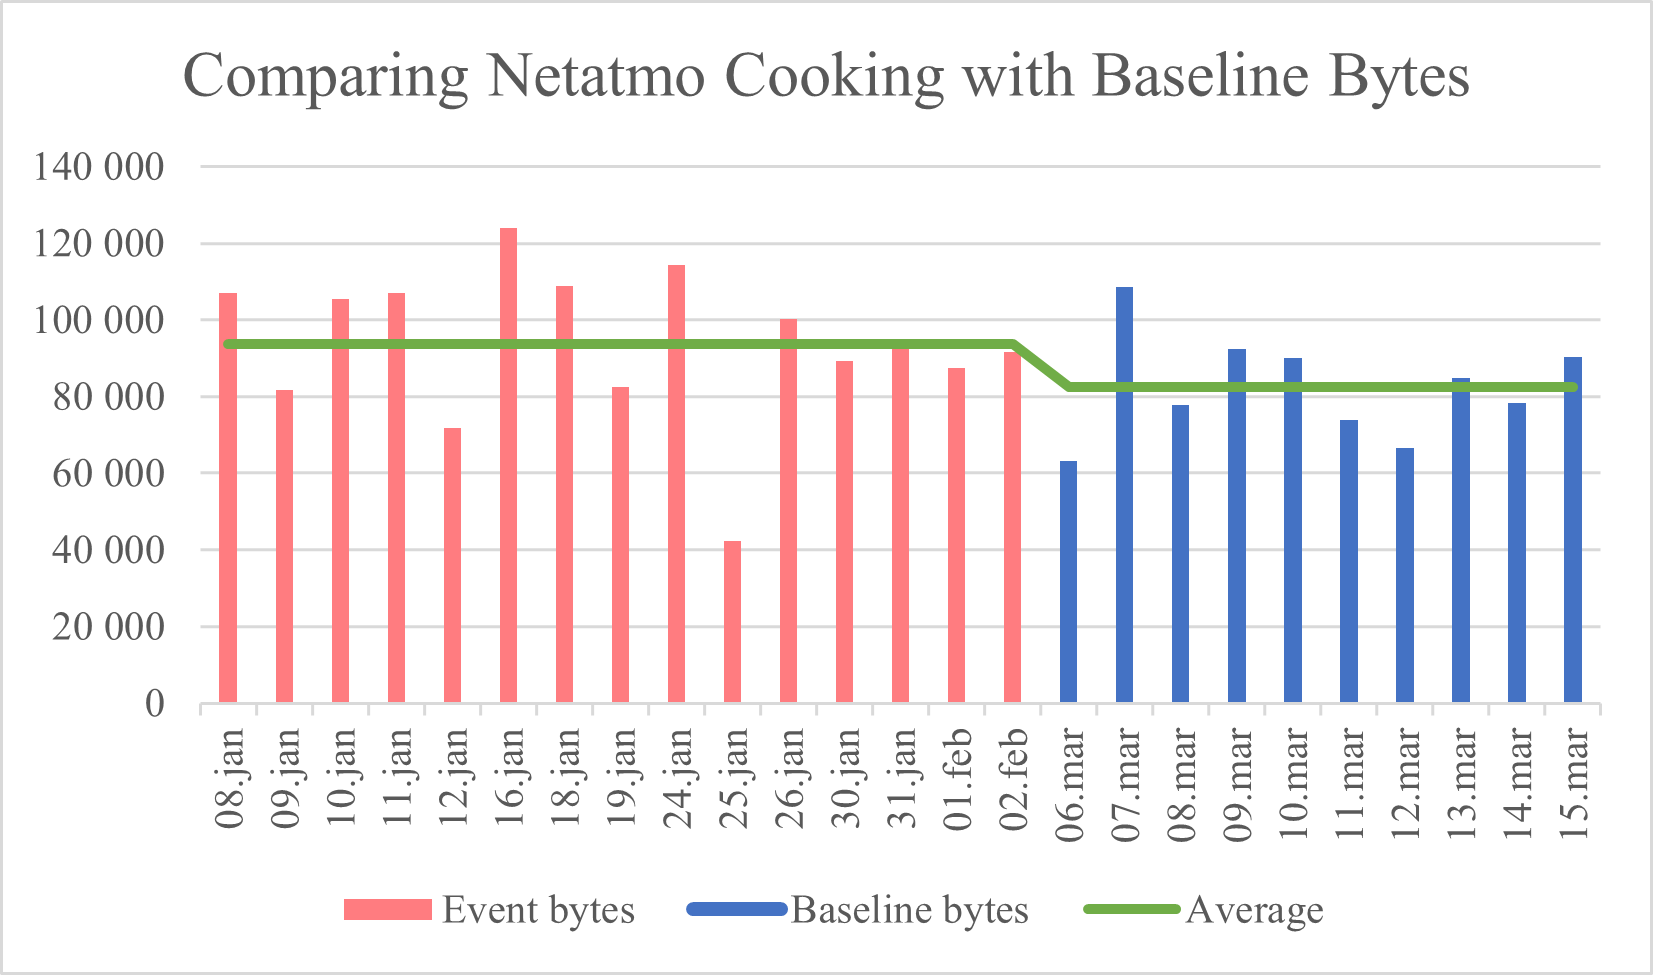
\includegraphics[width=1\hsize]{figures/Netatmo_Comparing_Cooking_Calculations_Bytes.png} 
    \end{subfigure}
    \begin{subfigure}{0.49\textwidth}
        \centering
        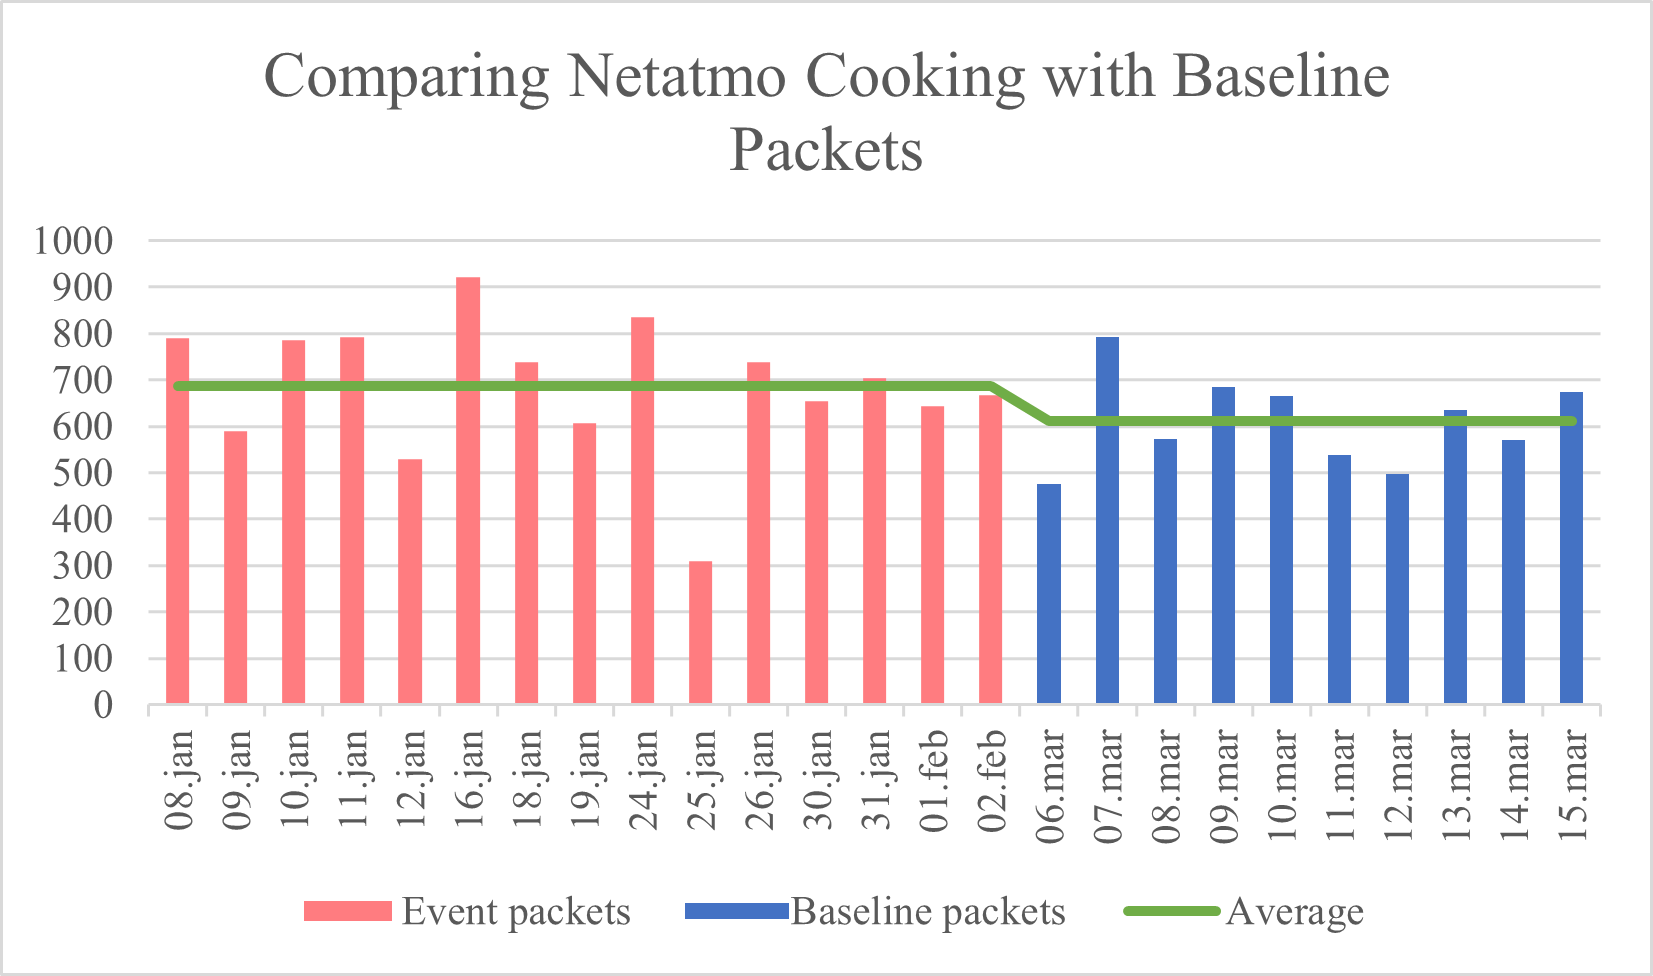
\includegraphics[width=1\hsize]{figures/Netatmo_Comparing_Cooking_Calculations_Packets.png} 
    \end{subfigure}
    \caption{Comparing Cooking Calculations for Netatmo}
    \label{fig:NetatmoComparingCookingCalculations}
\end{figure}

\subsection{Mill Sense}
The graphs in figure \ref{fig:MillCookingBytes} and \ref{fig:MillCookingPackets} shows both bytes and packets for the first 10 of the cooking events. The area marked red on the graphs are when the event was ongoing. Table \ref{tab:MillCookingCalculations} presents the calculations from all the 15 cooking events. 

\begin{table}[!ht]
    \centering
    \caption{Mill Cooking Calculations}
    \begin{tabular}{|l|l|l|l|l|l|}
    \hline
        \textbf{Events} & \textbf{Packets} & \textbf{Bytes} & \textbf{Biggest packet} \\ \hline
        08.jan & 7,729 & 945,461 & 456 bytes \\ \hline
        09.jan & 6,328 & 863,911 & 456 bytes \\ \hline
        10.jan & 6,821 & 916,827 & 456 bytes \\ \hline
        11.jan & 9,457 & 1,218,558 & 456 bytes \\ \hline
        12.jan & 7,600 & 965,797 & 456 bytes \\ \hline
        16.jan & 8,416 & 1,155,609 & 1,353 bytes \\ \hline
        18.jan & 7,589 & 938,903 & 456 bytes \\ \hline
        19.jan & 7,075 & 872,150 & 1,593 bytes \\ \hline
        24.jan & 9,395 & 1,129,302 & 1,593 bytes \\ \hline
        25.jan & 5,818 & 734,000 & 1,583 bytes \\ \hline
        26.jan & 8,240 & 1,056,828 & 1,593 bytes \\ \hline
        30.jan & 9,285 & 1,067,084 & 456 bytes  \\ \hline
        31.jan & 8,623 & 991,377 & 456 bytes \\ \hline
        01.feb & 8,678 & 1,026 864 & 456 bytes \\ \hline
        02.feb & 7,764 & 951,239 & 456 bytes \\ \hline
        \textbf{Average} & \textbf{7,921} & \textbf{988,927} & \textbf{818 bytes} \\ \hline
        \textbf{Std dev} & \textbf{1,101} & \textbf{124,838} & \textbf{533 bytes} \\ \hline
    \end{tabular}
    \label{tab:MillCookingCalculations}
\end{table}

\begin{figure}[H]
    \centering
    \begin{subfigure}{0.49\textwidth}
        \centering
        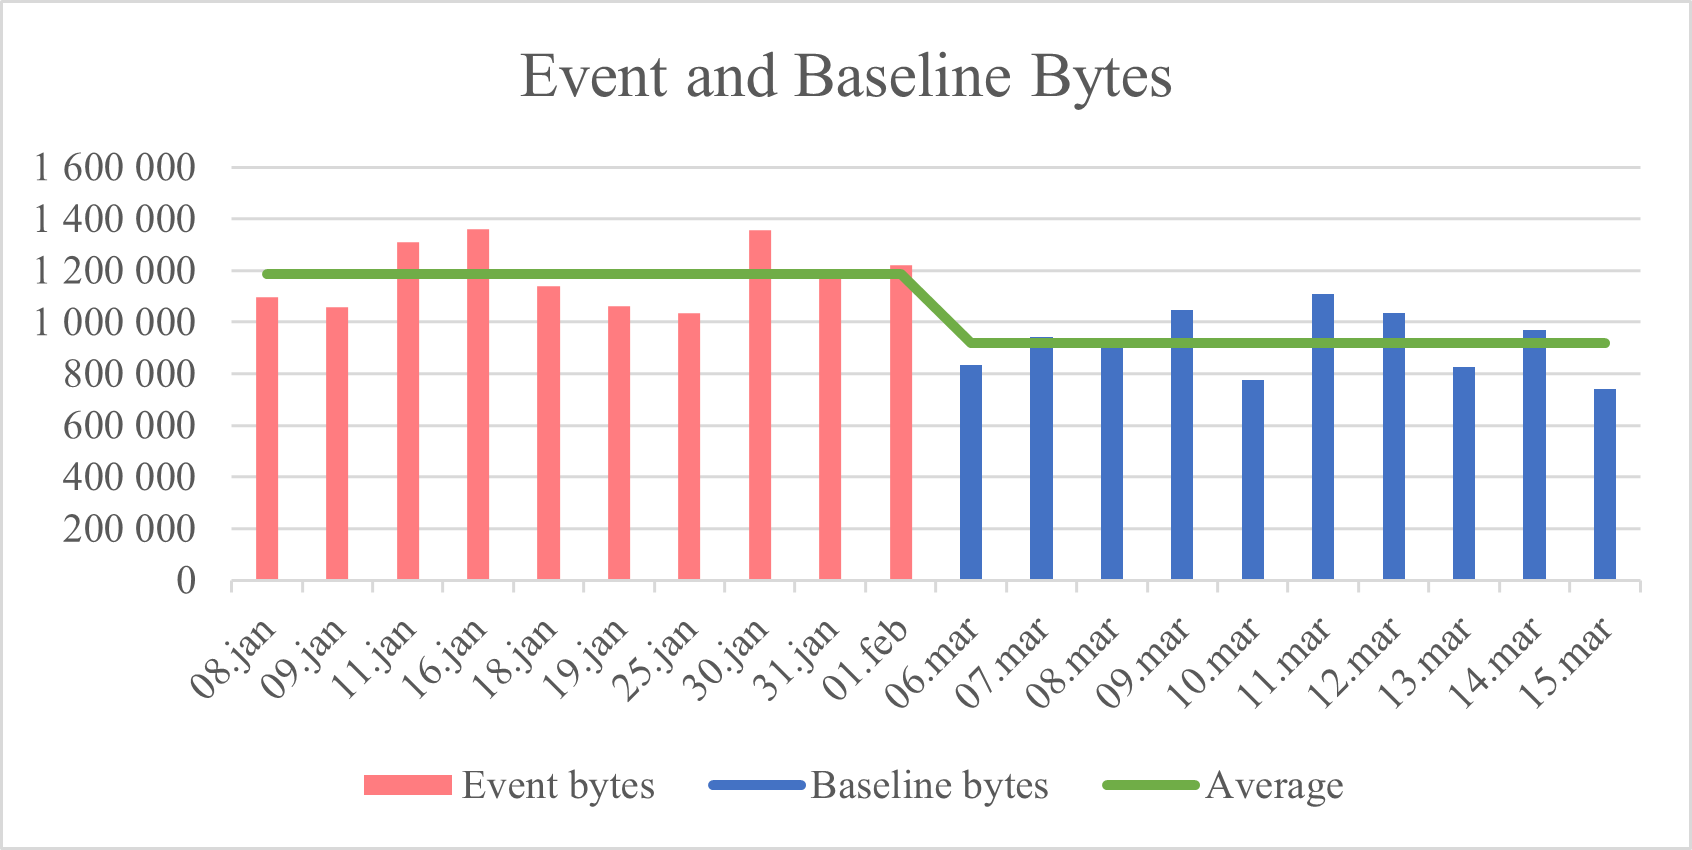
\includegraphics[width=1\hsize]{figures/Mill_Cooking_Calculations_Bytes.png} 
    \end{subfigure}
    \begin{subfigure}{0.49\textwidth}
        \centering
        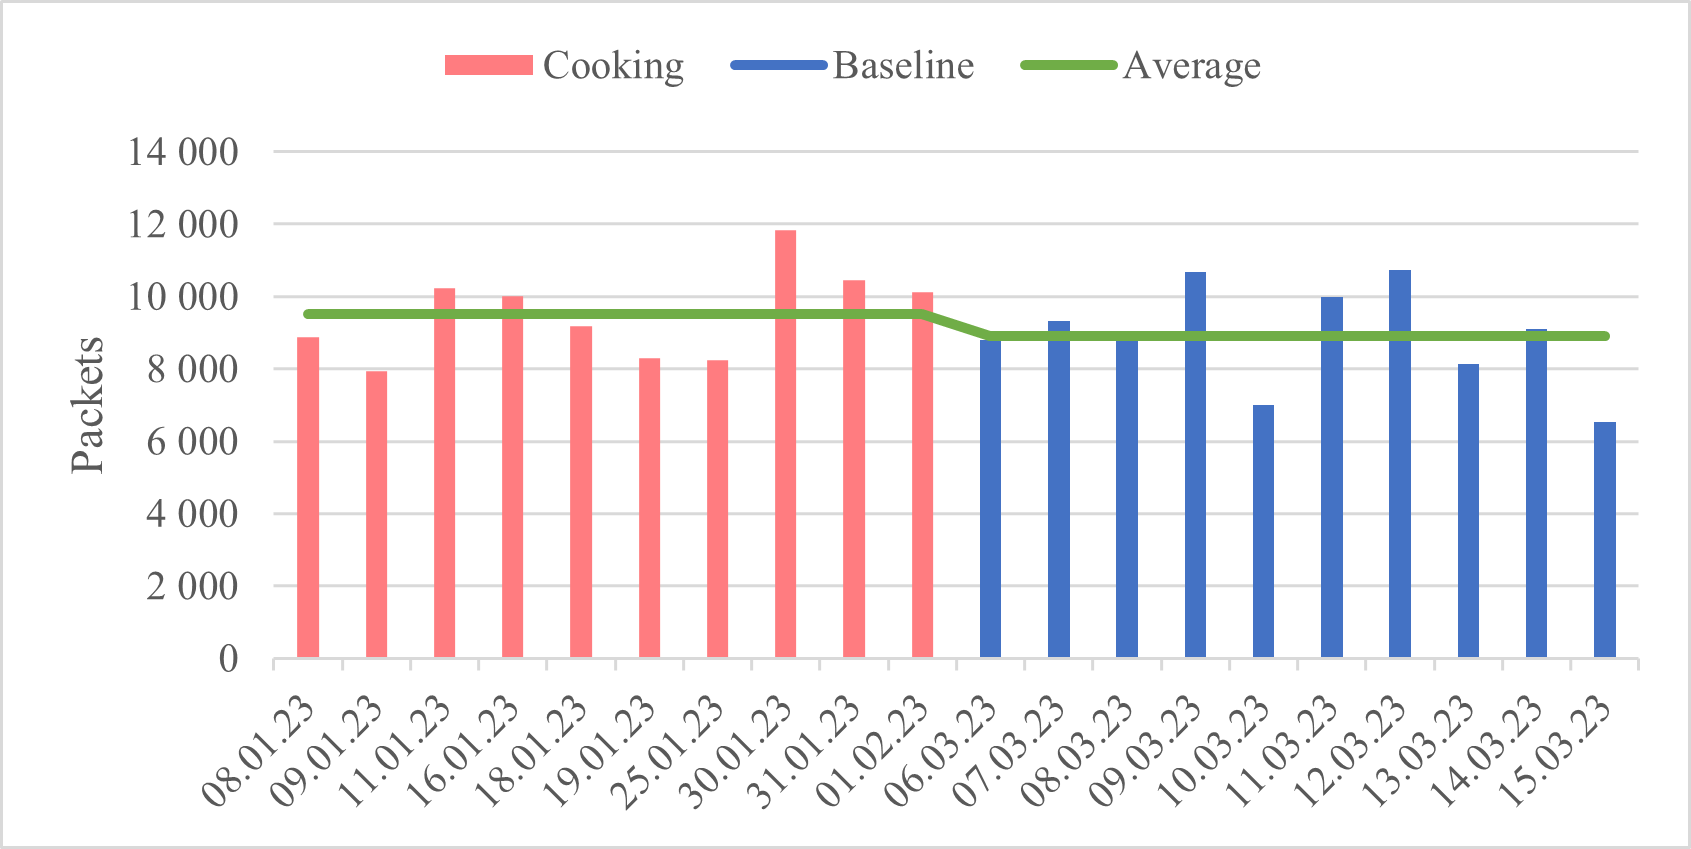
\includegraphics[width=1\hsize]{figures/Mill_Cooking_Calculations_Packets.png} 
    \end{subfigure}
    \caption{Cooking Calculations for Mill}
    \label{fig:MillCookingCalculations}
\end{figure}

\begin{figure}[H]
    \begin{subfigure}[b]{0.47\textwidth}
        \centering
        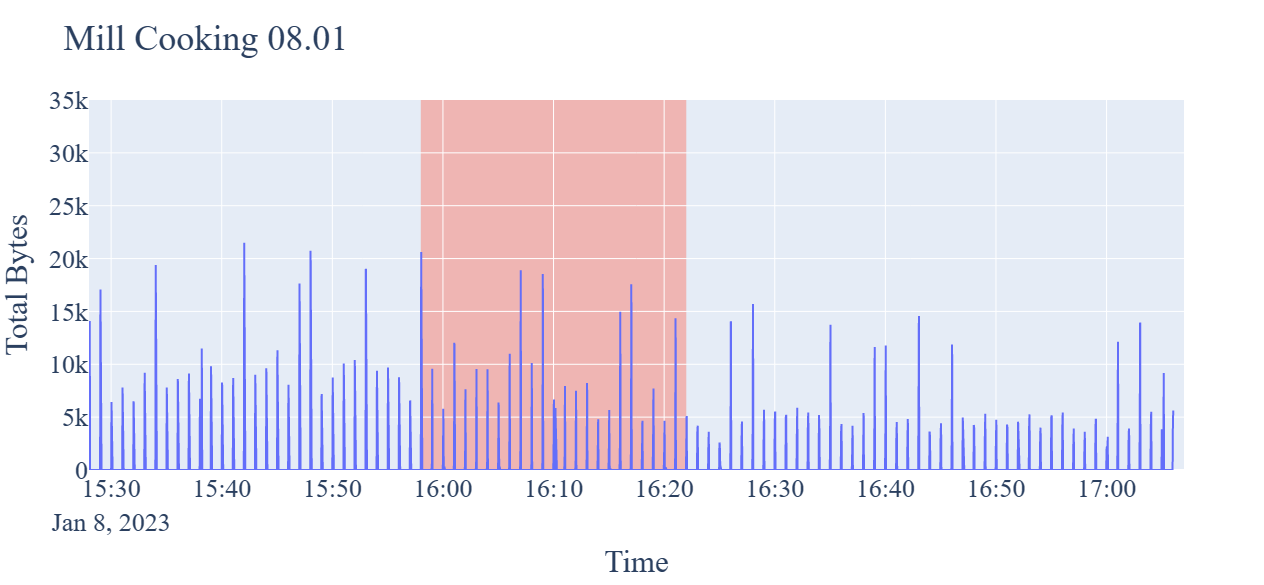
\includegraphics[width=1.2\hsize]{figures/Mill_Cooking_Bytes_08.01.png}
    \end{subfigure}
    \begin{subfigure}[b]{0.47\textwidth}
        \centering
        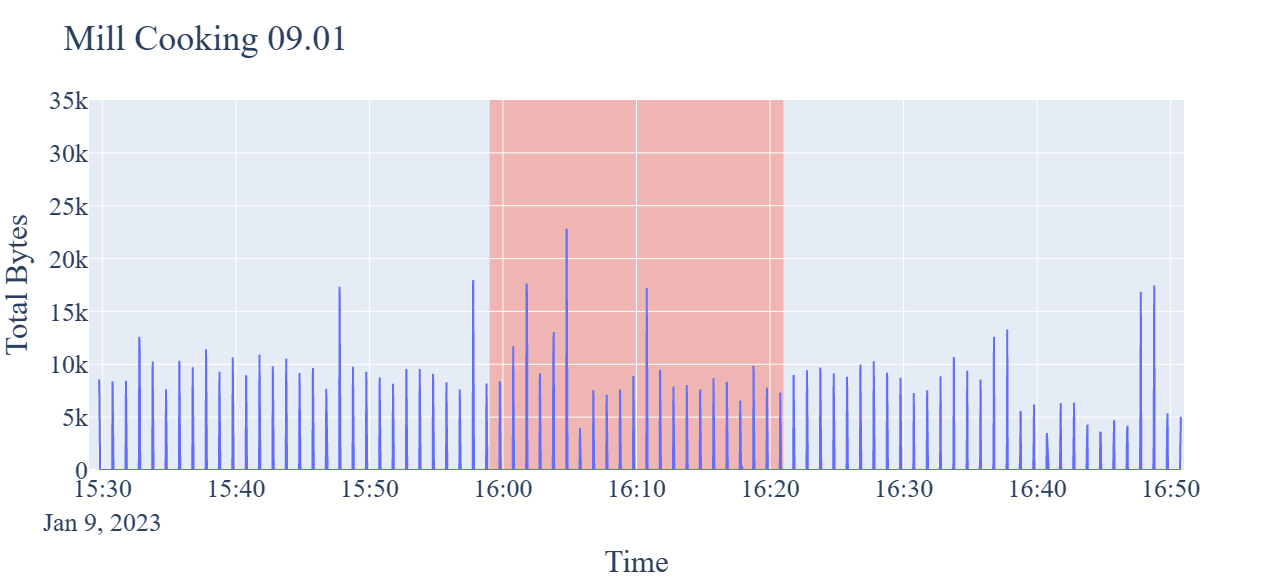
\includegraphics[width=1.2\hsize]{figures/Mill_Cooking_Bytes_09.01.png}
    \end{subfigure}
    \begin{subfigure}[b]{0.47\textwidth}
        \centering
        \includegraphics[width=1.2\hsize]{figures/Mill_Cooking_Bytes_10.01.png}
    \end{subfigure}
    \begin{subfigure}[b]{0.47\textwidth}
        \centering
        \includegraphics[width=1.2\hsize]{figures/Mill_Cooking_Bytes_11.01.png}
    \end{subfigure}
    \begin{subfigure}[b]{0.47\textwidth}
        \centering
        \includegraphics[width=1.2\hsize]{figures/Mill_Cooking_Bytes_12.01.png}
    \end{subfigure}
    \begin{subfigure}[b]{0.47\textwidth}
        \centering
        \includegraphics[width=1.2\hsize]{figures/Mill_Cooking_Bytes_16.01.png}
    \end{subfigure}
    \begin{subfigure}[b]{0.47\textwidth}
        \centering
        \includegraphics[width=1.2\hsize]{figures/Mill_Cooking_Bytes_18.01.png}
    \end{subfigure}
    \begin{subfigure}[b]{0.47\textwidth}
        \centering
        \includegraphics[width=1.2\hsize]{figures/Mill_Cooking_Bytes_19.01.png}
    \end{subfigure}
    \begin{subfigure}[b]{0.47\textwidth}
        \centering
        \includegraphics[width=1.2\hsize]{figures/Mill_Cooking_Bytes_24.01.png}
    \end{subfigure}
    \begin{subfigure}[b]{0.47\textwidth}
        \centering
        \includegraphics[width=1.2\hsize]{figures/Mill_Cooking_Bytes_25.01.png}
    \end{subfigure}
    \begin{subfigure}[b]{0.47\textwidth}
        \centering
        \includegraphics[width=1.2\hsize]{figures/Mill_Cooking_Bytes_26.01.png}
    \end{subfigure}
    \hspace{0.6cm}
    \begin{subfigure}[b]{0.47\textwidth}
        \centering
        \includegraphics[width=1.2\hsize]{figures/Mill_Cooking_Bytes_30.01.png}
    \end{subfigure}
    \caption{Mill Cooking Events - Bytes}
    \label{fig:MillCookingBytes}
\end{figure}

\begin{figure}[H]
    \begin{subfigure}[b]{0.47\textwidth}
        \centering
        \includegraphics[width=1.2\hsize]{figures/Mill_Cooking_Packets_08.01.png}
    \end{subfigure}
    \begin{subfigure}[b]{0.47\textwidth}
        \centering
        \includegraphics[width=1.2\hsize]{figures/Mill_Cooking_Packets_09.01.png}
    \end{subfigure}
    \begin{subfigure}[b]{0.47\textwidth}
        \centering
        \includegraphics[width=1.2\hsize]{figures/Mill_Cooking_Packets_10.01.png}
    \end{subfigure}
    \begin{subfigure}[b]{0.47\textwidth}
        \centering
        \includegraphics[width=1.2\hsize]{figures/Mill_Cooking_Packets_11.01.png}
    \end{subfigure}
    \begin{subfigure}[b]{0.47\textwidth}
        \centering
        \includegraphics[width=1.2\hsize]{figures/Mill_Cooking_Packets_12.01.png}
    \end{subfigure}
    \begin{subfigure}[b]{0.47\textwidth}
        \centering
        \includegraphics[width=1.2\hsize]{figures/Mill_Cooking_Packets_16.01.png}
    \end{subfigure}
    \begin{subfigure}[b]{0.47\textwidth}
        \centering
        \includegraphics[width=1.2\hsize]{figures/Mill_Cooking_Packets_18.01.png}
    \end{subfigure}
    \begin{subfigure}[b]{0.47\textwidth}
        \centering
        \includegraphics[width=1.2\hsize]{figures/Mill_Cooking_Packets_19.01.png}
    \end{subfigure}
    \begin{subfigure}[b]{0.47\textwidth}
        \centering
        \includegraphics[width=1.2\hsize]{figures/Mill_Cooking_Packets_24.01.png}
    \end{subfigure}
    \begin{subfigure}[b]{0.47\textwidth}
        \centering
        \includegraphics[width=1.2\hsize]{figures/Mill_Cooking_Packets_26.01.png}
    \end{subfigure}
    \begin{subfigure}[b]{0.47\textwidth}
        \centering
        \includegraphics[width=1.2\hsize]{figures/Mill_Cooking_Packets_26.01.png}
    \end{subfigure}
    \hspace{0.6cm}
    \begin{subfigure}[b]{0.47\textwidth}
        \centering
        \includegraphics[width=1.2\hsize]{figures/Mill_Cooking_Packets_30.01.png}
    \end{subfigure}
    \caption{Mill Cooking Events - Packets}
    \label{fig:MillCookingPackets}
\end{figure}

From the figures in \ref{fig:MillCookingBytes} and \ref{fig:MillCookingPackets} it is not possible to see a significant difference in the traffic when the event occurs to before and after the event. When looking at table \ref{tab:MillCookingCalculations}, the standard deviation shows that the values varies a lot. Packets varies from 5,818 to 9,457 packets and bytes varies from 1,218,558 to 734,000 bytes during the pcap for the event. The biggest packet sent switches between 456 bytes to around 1.500 bytes, therefore the average value here is a number close to the middle of those two numbers. Looking at the graphs in figure \ref{fig:MillCookingCalculations} shows how each event differs from each other and the average value. 
\\\\
The next step is to compare the figures and calculations from the events to the traffic captured from the baseline. Figure \ref{fig:MillCookingComparingBytes} and \ref{fig:MillCookingComparingPackets} compares the graphs for cooking from the actual events of Mill, marked in red, to the baseline capture of Mill, marked in blue. 

\begin{figure}[H]
    \begin{subfigure}[b]{0.47\textwidth}
        \centering
        \tcbincludegraphics[size=fbox,width=1.1\hsize,colframe=red]{figures/Mill_Cooking_Packets_08.01.png}
    \end{subfigure}
    \begin{subfigure}[b]{0.47\textwidth}
        \centering
        \tcbincludegraphics[size=fbox,width=1.1\hsize,colframe=blue]{figures/Mill_Cooking_Baseline_Packets_06.03.png}
    \end{subfigure}
    \begin{subfigure}[b]{0.47\textwidth}
        \centering
        \tcbincludegraphics[size=fbox,width=1.1\hsize,colframe=red]{figures/Mill_Cooking_Packets_10.01.png}
    \end{subfigure}
    \begin{subfigure}[b]{0.47\textwidth}
        \centering
        \tcbincludegraphics[size=fbox,width=1.1\hsize,colframe=blue]{figures/Mill_Cooking_Baseline_Packets_07.03.png}
    \end{subfigure}
    \begin{subfigure}[b]{0.47\textwidth}
        \centering
        \tcbincludegraphics[size=fbox,width=1.1\hsize,colframe=red]{figures/Mill_Cooking_Packets_12.01.png}
    \end{subfigure}
    \begin{subfigure}[b]{0.47\textwidth}
        \centering
        \tcbincludegraphics[size=fbox,width=1.1\hsize,colframe=blue]{figures/Mill_Cooking_Baseline_Packets_08.03.png}
    \end{subfigure}
    \begin{subfigure}[b]{0.47\textwidth}
        \centering
        \tcbincludegraphics[size=fbox,width=1.1\hsize,colframe=red]{figures/Mill_Cooking_Packets_18.01.png}
    \end{subfigure}
    \begin{subfigure}[b]{0.47\textwidth}
        \centering
        \tcbincludegraphics[size=fbox,width=1.1\hsize,colframe=blue]{figures/Mill_Cooking_Baseline_Packets_09.03.png}
    \end{subfigure}
    \begin{subfigure}[b]{0.47\textwidth}
        \centering
        \tcbincludegraphics[size=fbox,width=1.1\hsize,colframe=red]{figures/Mill_Cooking_Packets_24.01.png}
    \end{subfigure}
    \begin{subfigure}[b]{0.47\textwidth}
        \centering
        \tcbincludegraphics[size=fbox,width=1.1\hsize,colframe=blue]{figures/Mill_Cooking_Baseline_Packets_10.03.png}
    \end{subfigure}
        \begin{subfigure}[b]{0.47\textwidth}
        \centering
        \tcbincludegraphics[size=fbox,width=1.1\hsize,colframe=red]{figures/Mill_Cooking_Packets_26.01.png}
    \end{subfigure}
    \begin{subfigure}[b]{0.47\textwidth}
        \centering
        \tcbincludegraphics[size=fbox,width=1.1\hsize,colframe=blue]{figures/Mill_Cooking_Baseline_Packets_11.03.png}
    \end{subfigure}
    \begin{subfigure}[b]{0.47\textwidth}
        \centering
        \tcbincludegraphics[size=fbox,width=1.1\hsize,colframe=red]{figures/Mill_Cooking_Packets_30.01.png}
    \end{subfigure}
    \hspace{0.6cm}
    \begin{subfigure}[b]{0.47\textwidth}
    \centering
        \tcbincludegraphics[size=fbox,width=1.1\hsize,colframe=blue]{figures/Mill_Cooking_Baseline_Packets_12.03.png}
        \end{subfigure}
    \caption{Comparing Events and Baseline Packets for Cooking - Mill}
    \label{fig:MillCookingComparingPackets}
\end{figure}

\begin{figure}[H]
    \begin{subfigure}[b]{0.47\textwidth}
        \centering
        \tcbincludegraphics[size=fbox,width=1.1\hsize,colframe=red]{figures/Mill_Cooking_Bytes_08.01.png}
    \end{subfigure}
    \begin{subfigure}[b]{0.47\textwidth}
        \centering
        \tcbincludegraphics[size=fbox,width=1.1\hsize,colframe=blue]{figures/Mill_Cooking_Baseline_Bytes_06.03.png}
    \end{subfigure}
    \begin{subfigure}[b]{0.47\textwidth}
        \centering
        \tcbincludegraphics[size=fbox,width=1.1\hsize,colframe=red]{figures/Mill_Cooking_Bytes_10.01.png}
    \end{subfigure}
    \begin{subfigure}[b]{0.47\textwidth}
        \centering
        \tcbincludegraphics[size=fbox,width=1.1\hsize,colframe=blue]{figures/Mill_Cooking_Baseline_Bytes_07.03.png}
    \end{subfigure}
    \begin{subfigure}[b]{0.47\textwidth}
        \centering
        \tcbincludegraphics[size=fbox,width=1.1\hsize,colframe=red]{figures/Mill_Cooking_Bytes_12.01.png}
    \end{subfigure}
    \begin{subfigure}[b]{0.47\textwidth}
        \centering
        \tcbincludegraphics[size=fbox,width=1.1\hsize,colframe=blue]{figures/Mill_Cooking_Baseline_Bytes_08.03.png}
    \end{subfigure}
    \begin{subfigure}[b]{0.47\textwidth}
        \centering
        \tcbincludegraphics[size=fbox,width=1.1\hsize,colframe=red]{figures/Mill_Cooking_Bytes_18.01.png}
    \end{subfigure}
    \begin{subfigure}[b]{0.47\textwidth}
        \centering
        \tcbincludegraphics[size=fbox,width=1.1\hsize,colframe=blue]{figures/Mill_Cooking_Baseline_Bytes_09.03.png}
    \end{subfigure}
    \begin{subfigure}[b]{0.47\textwidth}
        \centering
        \tcbincludegraphics[size=fbox,width=1.1\hsize,colframe=red]{figures/Mill_Cooking_Bytes_24.01.png}
    \end{subfigure}
    \begin{subfigure}[b]{0.47\textwidth}
        \centering
        \tcbincludegraphics[size=fbox,width=1.1\hsize,colframe=blue]{figures/Mill_Cooking_Baseline_Bytes_10.03.png}
    \end{subfigure}
        \begin{subfigure}[b]{0.47\textwidth}
        \centering
        \tcbincludegraphics[size=fbox,width=1.1\hsize,colframe=red]{figures/Mill_Cooking_Bytes_26.01.png}
    \end{subfigure}
    \begin{subfigure}[b]{0.47\textwidth}
        \centering
        \tcbincludegraphics[size=fbox,width=1.1\hsize,colframe=blue]{figures/Mill_Cooking_Baseline_Bytes_11.03.png}
    \end{subfigure}
    \begin{subfigure}[b]{0.47\textwidth}
        \centering
        \tcbincludegraphics[size=fbox,width=1.1\hsize,colframe=red]{figures/Mill_Cooking_Bytes_30.01.png}
    \end{subfigure}
    \hspace{0.6cm}
    \begin{subfigure}[b]{0.47\textwidth}
    \centering
        \tcbincludegraphics[size=fbox,width=1.1\hsize,colframe=blue]{figures/Mill_Cooking_Baseline_Bytes_12.03.png}
        \end{subfigure}
    \caption{Comparing Events and Baseline Bytes for Cooking - Mill}
    \label{fig:MillCookingComparingBytes}
\end{figure}

From the graphs in figure \ref{fig:MillCookingComparingBytes} and \ref{fig:MillCookingComparingPackets} it is hard to see differences from the baseline and event traffic. It can therefore be beneficial to look at the calculations and see if there are any differences here. Table \ref{tab:MillBaselineCookingCalculations} presents the same calculations as for the events, but on the corresponding baseline capture files. 

\begin{table}[H]
    \centering
    \caption{Mill Baseline Cooking Calculations}
    \begin{tabular}{|l|l|l|l|l|l|}
    \hline
        \textbf{Baseline} & \textbf{Packets} & \textbf{Bytes} & \textbf{Biggest packet} \\ \hline
        06.mar & 6,997 & 667,501 & 426 bytes \\ \hline
        07.mar & 7,223 & 742,991 & 1,343 bytes \\ \hline
        08.mar & 7,037 & 724,183 & 1,343 bytes \\ \hline
        09.mar & 8,696 & 841,752 & 456 bytes \\ \hline
        10.mar & 5,583 & 593,772 & 424 bytes \\ \hline
        11.mar & 8,211 & 905,262 & 456 bytes \\ \hline
        12.mar & 9,051 & 850,503 & 456 bytes \\ \hline
        13.mar & 6,795 & 686,949 & 426 bytes \\ \hline
        14.mar & 7,268 & 761,018 & 1,573 bytes \\ \hline
        15.mar & 5,118 & 582,360 & 426 bytes \\ \hline
        \textbf{Average} &  \textbf{7,198}  &  \textbf{735,629}  &  \textbf{733 bytes} \\ \hline
        \textbf{Std dev}  &  \textbf{1,242}   &  \textbf{107,852}   &  \textbf{478 bytes} \\ \hline
    \end{tabular}
    \label{tab:MillBaselineCookingCalculations}
\end{table}

\begin{table}[H]
    \centering
    \caption{Comparing Cooking and Baseline Calculations for Mill}
    \begin{tabular}{c|l|l|l|l|}
        \cline{2-5}
        \multicolumn{1}{l|}{}                                              & \textbf{Type} & \textbf{Packets} & \textbf{Bytes} & \textbf{Biggest packet} \\ \hline
        \multicolumn{1}{|c|}{\multirow{2}{*}{\textbf{Average}}}            & Event         & 7,921              & 988,927        & 818 bytes               \\ \cline{2-5} 
        \multicolumn{1}{|c|}{}                                             & Baseline      & 7,198              & 735,629         & 733 bytes                \\ \hline
        \multicolumn{1}{|c|}{\multirow{2}{*}{\textbf{Standard deviation}}} & Event         & 1,101              & 124,838         & 533 bytes                 \\ \cline{2-5} 
        \multicolumn{1}{|c|}{}                                             & Baseline      & 1,242               & 107,852        &  478 bytes               \\ \hline          
    \end{tabular}
    \label{tab:MillComparingBaselineAndCookingCalculations}
\end{table}

\begin{figure}[H]
    \centering
    \begin{subfigure}{0.49\textwidth}
        \centering
        \includegraphics[width=1\hsize]{figures/Mill_Comparing_Cooking_Calculations_Bytes.png} 
    \end{subfigure}
    \begin{subfigure}{0.49\textwidth}
        \centering
        \includegraphics[width=1\hsize]{figures/Mill_Comparing_Cooking_Calculations_Packets.png} 
    \end{subfigure}
    \caption{Comparing Cooking Calculations for Mill}
    \label{fig:MillComparingCookingCalc
    ulations}
\end{figure}

\newpage
\subsection{Nedis}
Table \ref{tab:NedisCookingCalculations} shows the calculations made on the cooking events for Nedis, including total amount of packeta and bytes and biggest packet sent within each event. The graphs in Figure \ref{fig:NedisCookingCalculations} presents both packets and bytes for the cooking event compared to the average value. The graphs in Figure \ref{fig:NedisCookingBytes} and \ref{fig:NedisCookingPackets} shows both bytes and packets for the first 10 of the cooking events. The area marked red on the graphs are when the event was ongoing.

\begin{table}[H]
\centering
\caption{Nedis Cooking Calculations}
\label{tab:NedisCookingCalculations}
\begin{tabular}{|l|l|l|l|}
\hline
                   & \textbf{Packets} & \textbf{Bytes}     & \textbf{Biggest packet} \\ \hline
08.jan             & 20,926           & 2,834,097          & 485 bytes               \\ \hline
09.jan             & 21,766           & 3,202,040          & 424 bytes               \\ \hline
10.jan             & 22,696           & 2,870,057          & 424 bytes               \\ \hline
11.jan             & 22,770           & 3,306,458          & 424 bytes               \\ \hline
12.jan             & 19,981           & 2,805,340          & 485 bytes               \\ \hline
16.jan             & 20,702           & 3,082,977          & 485 bytes               \\ \hline
18.jan             & 21,292           & 2,689,055          & 424 bytes               \\ \hline
19.jan             & 16,247           & 2,500,650          & 424 bytes               \\ \hline
24.jan             & 27,549           & 3,758,598          & 485 bytes               \\ \hline
25.jan             & 17,759           & 2,308,623          & 424 bytes               \\ \hline
26.jan             & 22,457           & 3,016,625          & 424 bytes               \\ \hline
30.jan             & 19,563           & 2,540,731          & 424 bytes               \\ \hline
31.jan             & 18,587           & 2,487,586          & 424 bytes               \\ \hline
01.feb             & 20,844           & 2,878,197          & 424 bytes               \\ \hline
02.feb             & 23,426           & 3,283,178          & 424 bytes               \\ \hline
\textbf{Average}   & \textbf{21,104}  & \textbf{2,904,281} & \textbf{440 bytes}      \\ \hline
\textbf{Std dev} & \textbf{2,667}   & \textbf{383,108}   & \textbf{28 bytes}         \\ \hline
\end{tabular}
\end{table}

\begin{figure}[H]
    \centering
    \begin{subfigure}{0.49\textwidth}
        \centering
        \includegraphics[width=1\hsize]{figures/Nedis_Cooking_Calculations_Bytes.png} 
    \end{subfigure}
    \begin{subfigure}{0.49\textwidth}
        \centering
        \includegraphics[width=1\hsize]{figures/Nedis_Cooking_Calculations_Packets.png} 
    \end{subfigure}
    \caption{Cooking Calculations for Nedis}
    \label{fig:NedisCookingCalculations}
\end{figure}

\begin{figure}[H]
    \begin{subfigure}[b]{0.47\textwidth}
        \centering
        \includegraphics[width=1.2\hsize]{figures/Nedis_Cooking_Bytes_08.01.png}
    \end{subfigure}
    \begin{subfigure}[b]{0.47\textwidth}
        \centering
        \includegraphics[width=1.2\hsize]{figures/Nedis_Cooking_Bytes_09.01.png}
    \end{subfigure}
    \begin{subfigure}[b]{0.47\textwidth}
        \centering
        \includegraphics[width=1.2\hsize]{figures/Nedis_Cooking_Bytes_10.01.png}
    \end{subfigure}
    \begin{subfigure}[b]{0.47\textwidth}
        \centering
        \includegraphics[width=1.2\hsize]{figures/Nedis_Cooking_Bytes_11.01.png}
    \end{subfigure}
    \begin{subfigure}[b]{0.47\textwidth}
        \centering
        \includegraphics[width=1.2\hsize]{figures/Nedis_Cooking_Bytes_12.01.png}
    \end{subfigure}
    \begin{subfigure}[b]{0.47\textwidth}
        \centering
        \includegraphics[width=1.2\hsize]{figures/Nedis_Cooking_Bytes_16.01.png}
    \end{subfigure}
    \begin{subfigure}[b]{0.47\textwidth}
        \centering
        \includegraphics[width=1.2\hsize]{figures/Nedis_Cooking_Bytes_18.01.png}
    \end{subfigure}
    \begin{subfigure}[b]{0.47\textwidth}
        \centering
        \includegraphics[width=1.2\hsize]{figures/Nedis_Cooking_Bytes_19.01.png}
    \end{subfigure}
    \begin{subfigure}[b]{0.47\textwidth}
        \centering
        \includegraphics[width=1.2\hsize]{figures/Nedis_Cooking_Bytes_24.01.png}
    \end{subfigure}
    \begin{subfigure}[b]{0.47\textwidth}
        \centering
        \includegraphics[width=1.2\hsize]{figures/Nedis_Cooking_Bytes_25.01.png}
    \end{subfigure}
    \begin{subfigure}[b]{0.47\textwidth}
        \centering
        \includegraphics[width=1.2\hsize]{figures/Nedis_Cooking_Bytes_26.01.png}
    \end{subfigure}
    \hspace{0.6cm}
    \begin{subfigure}[b]{0.47\textwidth}
        \centering
        \includegraphics[width=1.2\hsize]{figures/Nedis_Cooking_Bytes_30.01.png}
    \end{subfigure}
    \caption{Nedis Cooking Events - Bytes}
    \label{fig:NedisCookingBytes}
\end{figure}

\begin{figure}[H]
    \begin{subfigure}[b]{0.47\textwidth}
        \centering
        \includegraphics[width=1.2\hsize]{figures/Nedis_Cooking_Packets_08.01.png}
    \end{subfigure}
    \begin{subfigure}[b]{0.47\textwidth}
        \centering
        \includegraphics[width=1.2\hsize]{figures/Nedis_Cooking_Packets_09.01.png}
    \end{subfigure}
    \begin{subfigure}[b]{0.47\textwidth}
        \centering
        \includegraphics[width=1.2\hsize]{figures/Nedis_Cooking_Packets_10.01.png}
    \end{subfigure}
    \begin{subfigure}[b]{0.47\textwidth}
        \centering
        \includegraphics[width=1.2\hsize]{figures/Nedis_Cooking_Packets_11.01.png}
    \end{subfigure}
    \begin{subfigure}[b]{0.47\textwidth}
        \centering
        \includegraphics[width=1.2\hsize]{figures/Nedis_Cooking_Packets_12.01.png}
    \end{subfigure}
    \begin{subfigure}[b]{0.47\textwidth}
        \centering
        \includegraphics[width=1.2\hsize]{figures/Nedis_Cooking_Packets_16.01.png}
    \end{subfigure}
    \begin{subfigure}[b]{0.47\textwidth}
        \centering
        \includegraphics[width=1.2\hsize]{figures/Nedis_Cooking_Packets_18.01.png}
    \end{subfigure}
    \begin{subfigure}[b]{0.47\textwidth}
        \centering
        \includegraphics[width=1.2\hsize]{figures/Nedis_Cooking_Packets_19.01.png}
    \end{subfigure}
    \begin{subfigure}[b]{0.47\textwidth}
        \centering
        \includegraphics[width=1.2\hsize]{figures/Nedis_Cooking_Packets_24.01.png}
    \end{subfigure}
    \begin{subfigure}[b]{0.47\textwidth}
        \centering
        \includegraphics[width=1.2\hsize]{figures/Nedis_Cooking_Packets_26.01.png}
    \end{subfigure}
    \begin{subfigure}[b]{0.47\textwidth}
        \centering
        \includegraphics[width=1.2\hsize]{figures/Nedis_Cooking_Packets_26.01.png}
    \end{subfigure}
    \hspace{0.6cm}
    \begin{subfigure}[b]{0.47\textwidth}
        \centering
        \includegraphics[width=1.2\hsize]{figures/Nedis_Cooking_Packets_30.01.png}
    \end{subfigure}
    \caption{Nedis Cooking Events - Packets}
    \label{fig:NedisCookingPackets}
\end{figure}

The graphs in Figure \ref{fig:NedisCookingBytes} and \ref{fig:NedisCookingPackets} does not show a significant change in traffic pattern during the event. The calculations in Table \ref{tab:NedisCookingCalculations} shows that the amount of packets does not vary that much with a standard deviation of 2,667 packets. The amount of bytes also has a small standard deviation, but the amount of bytes do vary from 2,308,623 to 3,306,458 bytes. The biggest packet for each event are either 424 or 485 bytes. The Figures in \ref{fig:NedisCookingCalculations} also shows that bytes and packets are close to the average value. 
\\\\
The next step is to compare the event calculations and graphs to the corresponding calculations and graphs from the baseline. Figure \ref{fig:NedisCookingComparingPackets} and \ref{fig:NedisCookingComparingBytes} compares these two, with the event graphs marked in red and the baseline graphs marked in blue, and compares for both packets and bytes. Table \ref{tab:NedisBaselineCookingCalculations} presents the same calculations for the baseline as Table \ref{tab:NedisCookingCalculations} does for the cooking events. Table \ref{tab:NedisComparingBaselineAndCookingCalculations} presents the average value and standard deviation of the baseline events and cooking events in a table to compare. Figure \ref{fig:NedisComparingCookingCalculations} gives a graphical comparison of baseline and cooking events with both packets and bytes.  
\newpage
\begin{figure}[H]
    \begin{subfigure}[b]{0.47\textwidth}
        \centering
        \tcbincludegraphics[size=fbox,width=1.1\hsize,colframe=red]{figures/Nedis_Cooking_Packets_08.01.png}
    \end{subfigure}
    \begin{subfigure}[b]{0.47\textwidth}
        \centering
        \tcbincludegraphics[size=fbox,width=1.1\hsize,colframe=blue]{figures/Nedis_Cooking_Baseline_Packets_06.03.png}
    \end{subfigure}
    \begin{subfigure}[b]{0.47\textwidth}
        \centering
        \tcbincludegraphics[size=fbox,width=1.1\hsize,colframe=red]{figures/Nedis_Cooking_Packets_10.01.png}
    \end{subfigure}
    \begin{subfigure}[b]{0.47\textwidth}
        \centering
        \tcbincludegraphics[size=fbox,width=1.1\hsize,colframe=blue]{figures/Nedis_Cooking_Baseline_Packets_07.03.png}
    \end{subfigure}
    \begin{subfigure}[b]{0.47\textwidth}
        \centering
        \tcbincludegraphics[size=fbox,width=1.1\hsize,colframe=red]{figures/Nedis_Cooking_Packets_12.01.png}
    \end{subfigure}
    \begin{subfigure}[b]{0.47\textwidth}
        \centering
        \tcbincludegraphics[size=fbox,width=1.1\hsize,colframe=blue]{figures/Nedis_Cooking_Baseline_Packets_08.03.png}
    \end{subfigure}
    \begin{subfigure}[b]{0.47\textwidth}
        \centering
        \tcbincludegraphics[size=fbox,width=1.1\hsize,colframe=red]{figures/Nedis_Cooking_Packets_18.01.png}
    \end{subfigure}
    \begin{subfigure}[b]{0.47\textwidth}
        \centering
        \tcbincludegraphics[size=fbox,width=1.1\hsize,colframe=blue]{figures/Nedis_Cooking_Baseline_Packets_09.03.png}
    \end{subfigure}
    \begin{subfigure}[b]{0.47\textwidth}
        \centering
        \tcbincludegraphics[size=fbox,width=1.1\hsize,colframe=red]{figures/Nedis_Cooking_Packets_24.01.png}
    \end{subfigure}
    \begin{subfigure}[b]{0.47\textwidth}
        \centering
        \tcbincludegraphics[size=fbox,width=1.1\hsize,colframe=blue]{figures/Nedis_Cooking_Baseline_Packets_10.03.png}
    \end{subfigure}
        \begin{subfigure}[b]{0.47\textwidth}
        \centering
        \tcbincludegraphics[size=fbox,width=1.1\hsize,colframe=red]{figures/Nedis_Cooking_Packets_26.01.png}
    \end{subfigure}
    \begin{subfigure}[b]{0.47\textwidth}
        \centering
        \tcbincludegraphics[size=fbox,width=1.1\hsize,colframe=blue]{figures/Nedis_Cooking_Baseline_Packets_11.03.png}
    \end{subfigure}
    \begin{subfigure}[b]{0.47\textwidth}
        \centering
        \tcbincludegraphics[size=fbox,width=1.1\hsize,colframe=red]{figures/Nedis_Cooking_Packets_30.01.png}
    \end{subfigure}
    \hspace{0.6cm}
    \begin{subfigure}[b]{0.47\textwidth}
    \centering
        \tcbincludegraphics[size=fbox,width=1.1\hsize,colframe=blue]{figures/Nedis_Cooking_Baseline_Packets_12.03.png}
        \end{subfigure}
    \caption{Comparing Events and Baseline Packets for Cooking - Nedis}
    \label{fig:NedisCookingComparingPackets}
\end{figure}

\begin{figure}[H]
    \begin{subfigure}[b]{0.47\textwidth}
        \centering
        \tcbincludegraphics[size=fbox,width=1.1\hsize,colframe=red]{figures/Nedis_Cooking_Bytes_08.01.png}
    \end{subfigure}
    \begin{subfigure}[b]{0.47\textwidth}
        \centering
        \tcbincludegraphics[size=fbox,width=1.1\hsize,colframe=blue]{figures/Nedis_Cooking_Baseline_Bytes_06.03.png}
    \end{subfigure}
    \begin{subfigure}[b]{0.47\textwidth}
        \centering
        \tcbincludegraphics[size=fbox,width=1.1\hsize,colframe=red]{figures/Nedis_Cooking_Bytes_10.01.png}
    \end{subfigure}
    \begin{subfigure}[b]{0.47\textwidth}
        \centering
        \tcbincludegraphics[size=fbox,width=1.1\hsize,colframe=blue]{figures/Nedis_Cooking_Baseline_Bytes_07.03.png}
    \end{subfigure}
    \begin{subfigure}[b]{0.47\textwidth}
        \centering
        \tcbincludegraphics[size=fbox,width=1.1\hsize,colframe=red]{figures/Nedis_Cooking_Bytes_12.01.png}
    \end{subfigure}
    \begin{subfigure}[b]{0.47\textwidth}
        \centering
        \tcbincludegraphics[size=fbox,width=1.1\hsize,colframe=blue]{figures/Nedis_Cooking_Baseline_Bytes_08.03.png}
    \end{subfigure}
    \begin{subfigure}[b]{0.47\textwidth}
        \centering
        \tcbincludegraphics[size=fbox,width=1.1\hsize,colframe=red]{figures/Nedis_Cooking_Bytes_18.01.png}
    \end{subfigure}
    \begin{subfigure}[b]{0.47\textwidth}
        \centering
        \tcbincludegraphics[size=fbox,width=1.1\hsize,colframe=blue]{figures/Nedis_Cooking_Baseline_Bytes_09.03.png}
    \end{subfigure}
    \begin{subfigure}[b]{0.47\textwidth}
        \centering
        \tcbincludegraphics[size=fbox,width=1.1\hsize,colframe=red]{figures/Nedis_Cooking_Bytes_24.01.png}
    \end{subfigure}
    \begin{subfigure}[b]{0.47\textwidth}
        \centering
        \tcbincludegraphics[size=fbox,width=1.1\hsize,colframe=blue]{figures/Nedis_Cooking_Baseline_Bytes_10.03.png}
    \end{subfigure}
        \begin{subfigure}[b]{0.47\textwidth}
        \centering
        \tcbincludegraphics[size=fbox,width=1.1\hsize,colframe=red]{figures/Nedis_Cooking_Bytes_26.01.png}
    \end{subfigure}
    \begin{subfigure}[b]{0.47\textwidth}
        \centering
        \tcbincludegraphics[size=fbox,width=1.1\hsize,colframe=blue]{figures/Nedis_Cooking_Baseline_Bytes_11.03.png}
    \end{subfigure}
    \begin{subfigure}[b]{0.47\textwidth}
        \centering
        \tcbincludegraphics[size=fbox,width=1.1\hsize,colframe=red]{figures/Nedis_Cooking_Bytes_30.01.png}
    \end{subfigure}
    \hspace{0.6cm}
    \begin{subfigure}[b]{0.47\textwidth}
    \centering
        \tcbincludegraphics[size=fbox,width=1.1\hsize,colframe=blue]{figures/Nedis_Cooking_Baseline_Bytes_12.03.png}
        \end{subfigure}
    \caption{Comparing Events and Baseline Bytes for Cooking - Nedis}
    \label{fig:NedisCookingComparingBytes}
\end{figure}

\begin{table}[]
\centering
\caption{Nedis Baseline Cooking Calculations}
\label{tab:NedisBaselineCookingCalculations}
\begin{tabular}{l|l|l|l|}
\cline{2-4}
                                       & \textbf{Packets}    & \textbf{Bytes}      & \textbf{Biggest packet} \\ \hline
\multicolumn{1}{|l|}{06.mar}           & 9,976                & 1,083,371             & 421 bytes        \\ \hline
\multicolumn{1}{|l|}{07.mar}           & 14,689               & 1,575,718             & 421 bytes         \\ \hline
\multicolumn{1}{|l|}{08.mar}           & 14,348               & 1,580,885             & 421 bytes         \\ \hline
\multicolumn{1}{|l|}{09.mar}           & 17,560               & 2,093,976             & 424 bytes         \\ \hline
\multicolumn{1}{|l|}{10.mar}           & 13,786               & 1,794,198             & 421 bytes         \\ \hline
\multicolumn{1}{|l|}{11.mar}           & 15,449               & 1,803,003             & 485 bytes         \\ \hline
\multicolumn{1}{|l|}{12.mar}           & 7,967                & 987,680              & 421 bytes          \\ \hline
\multicolumn{1}{|l|}{13.mar}           & 13,449               & 1,668,571             & 421 bytes         \\ \hline
\multicolumn{1}{|l|}{14.mar}           & 12,093               & 1,408,301             & 341 bytes         \\ \hline
\multicolumn{1}{|l|}{15.mar}           & 15,639               & 2,020,215             & 458 bytes         \\ \hline
\multicolumn{1}{|l|}{\textbf{Average}} & \textbf{13,496}      & \textbf{1,601,592}  & \textbf{423 bytes} \\ \hline
\multicolumn{1}{|l|}{\textbf{Std dev}} & \textbf{2,830} & \textbf{3,626,66} & \textbf{36 bytes}     \\ \hline
\end{tabular}
\end{table}

\begin{table}[H]
    \centering
    \caption{Comparing Cooking and Baseline Calculations for Nedis}
    \begin{tabular}{c|l|l|l|l|}
        \cline{2-5}
        \multicolumn{1}{l|}{}                                              & \textbf{Type} & \textbf{Packets} & \textbf{Bytes} & \textbf{Biggest packet} \\ \hline
        \multicolumn{1}{|c|}{\multirow{2}{*}{\textbf{Average}}}            & Event         & 21,104              & 2,904,281        & 440 bytes               \\ \cline{2-5} 
        \multicolumn{1}{|c|}{}                                             & Baseline      & 13,496              & 1,601,592         & 423 bytes                \\ \hline
        \multicolumn{1}{|c|}{\multirow{2}{*}{\textbf{Standard deviation}}} & Event         & 2,667              & 383,108         & 28 bytes                 \\ \cline{2-5} 
        \multicolumn{1}{|c|}{}                                             & Baseline      & 2.830               & 362,666        &  36 bytes               \\ \hline          
    \end{tabular}
    \label{tab:NedisComparingBaselineAndCookingCalculations}
\end{table}

\begin{figure}[H]
    \centering
    \begin{subfigure}{0.49\textwidth}
        \centering
        \includegraphics[width=1\hsize]{figures/Nedis_Comparing_Cooking_Calculations_Bytes.png} 
    \end{subfigure}
    \begin{subfigure}{0.49\textwidth}
        \centering
        \includegraphics[width=1\hsize]{figures/Nedis_Comparing_Cooking_Calculations_Packets.png} 
    \end{subfigure}
    \caption{Comparing Cooking Calculations for Nedis}
    \label{fig:NedisComparingCookingCalculations}
\end{figure}

\newpage
\section{Test Case 2: Showering}
This chapter presents the results and analysis conducted on Test Case 2: Showering. 
\subsection{General}
The showering event has been conducted 10 times and Table \ref{tab:ShoweringDates} presents the 10 different dates and exact times for when the event was ongoing.
\begin{table}[!hbtp]
    \centering
    \caption{Date and time for Test Case 2: Showering events}
    \begin{adjustbox}{width=1\textwidth} 
        \begin{tabular}{l|l|l|l|l|l|l|l|l|l|l|}
            \cline{2-11}
                & 08.01 & 09.01 & 11.01 & 16.01 & 18.01 & 19.01 & 25.01 & 30.01 & 31.01 & 01.02 \\ \hline
            \multicolumn{1}{|l|}{Started event}  & 19:59 & 20:14 & 20:01 & 20:12 & 20:02 & 20:00 & 20:03 & 20:00 & 20:01 & 20:00 \\ \hline
            \multicolumn{1}{|l|}{Finished event} & 20:14 & 20:34 & 20:17 & 20:31 & 20:19 & 20:16 & 20:19 & 20:18 & 20:17 & 20:16 \\ \hline
        \end{tabular}
    \end{adjustbox}
    \label{tab:ShoweringDates}
\end{table}

\subsection{Netatmo Home Coach}

\begin{table}[!ht]
    \centering
    \caption{Netatmo Shower Calculations}
    \begin{tabular}{l|l|l|l|l|l|}
        \cline{2-4}               & \textbf{Packets} & \textbf{Bytes} & \textbf{Biggest packet} \\ \hline
        \multicolumn{1}{|l|}{08.jan}           & 678          & 91,839         & 407 bytes      \\ \hline
        \multicolumn{1}{|l|}{09.jan}           & 678          & 93,005         & 407 bytes      \\ \hline
        \multicolumn{1}{|l|}{11.jan}           & 856          & 116,628        & 407 bytes      \\ \hline
        \multicolumn{1}{|l|}{16.jan}           & 514          & 70,004         & 407 bytes      \\ \hline
        \multicolumn{1}{|l|}{18.jan}           & 608          & 83,713         & 407 bytes      \\ \hline
        \multicolumn{1}{|l|}{19.jan}           & 503          & 68,174         & 407 bytes      \\ \hline
        \multicolumn{1}{|l|}{25.jan}           & 748          & 100,660        & 407 bytes      \\ \hline
        \multicolumn{1}{|l|}{30.jan}           & 716          & 96,957         & 407 bytes      \\ \hline
        \multicolumn{1}{|l|}{31.jan}           & 599          & 80,202         & 136 bytes      \\ \hline
        \multicolumn{1}{|l|}{01.feb}           & 545          & 73,695         & 407 bytes      \\ \hline
        \multicolumn{1}{|l|}{\textbf{Average}} & \textbf{645} & \textbf{87,488} & \textbf{380 bytes}   \\ \hline
        \multicolumn{1}{|l|}{\textbf{Std dev}} & \textbf{112} & \textbf{15,268} & \textbf{86 bytes}    \\ \hline
    \end{tabular}
    \label{tab:NetatmoShowerCalculations}
\end{table}

\begin{figure}[H]
    \centering
    \begin{subfigure}{0.49\textwidth}
       \includegraphics[width=1\hsize]{figures/Netatmo_Shower_Calculations_Packets.png} 
    \end{subfigure}
    \begin{subfigure}{0.49\textwidth}
        \includegraphics[width=1\hsize]{figures/Netatmo_Shower_Calculations_Bytes.png} 
    \end{subfigure}
    \caption{Graphical representation of packets and bytes with average values from Table \ref{tab:NetatmoShowerCalculations}}
    \label{fig:NetatmoShowerCalculations}
\end{figure}

\begin{figure}[H]
    \begin{subfigure}[b]{0.47\textwidth}
        \centering
        \includegraphics[width=1.2\hsize]{figures/Netatmo_Shower_Bytes_08.01.png}
    \end{subfigure}
    \begin{subfigure}[b]{0.47\textwidth}
        \centering
        \includegraphics[width=1.2\hsize]{figures/Netatmo_Shower_Bytes_09.01.png}
    \end{subfigure}
    \begin{subfigure}[b]{0.47\textwidth}
        \centering
        \includegraphics[width=1.2\hsize]{figures/Netatmo_Shower_Bytes_11.01.png}
    \end{subfigure}
    \begin{subfigure}[b]{0.47\textwidth}
        \centering
        \includegraphics[width=1.2\hsize]{figures/Netatmo_Shower_Bytes_16.01.png}
    \end{subfigure}
    \begin{subfigure}[b]{0.47\textwidth}
        \centering
        \includegraphics[width=1.2\hsize]{figures/Netatmo_Shower_Bytes_18.01.png}
    \end{subfigure}
    \begin{subfigure}[b]{0.47\textwidth}
        \centering
        \includegraphics[width=1.2\hsize]{figures/Netatmo_Shower_Bytes_19.01.png}
    \end{subfigure}
    \begin{subfigure}[b]{0.47\textwidth}
        \centering
        \includegraphics[width=1.2\hsize]{figures/Netatmo_Shower_Bytes_25.01.png}
    \end{subfigure}
    \begin{subfigure}[b]{0.47\textwidth}
        \centering
        \includegraphics[width=1.2\hsize]{figures/Netatmo_Shower_Bytes_30.01.png}
    \end{subfigure}
    \begin{subfigure}[b]{0.47\textwidth}
        \centering
        \includegraphics[width=1.2\hsize]{figures/Netatmo_Shower_Bytes_31.01.png}
    \end{subfigure}
    \hspace{0.6cm}
    \begin{subfigure}[b]{0.47\textwidth}
        \centering
        \includegraphics[width=1.2\hsize]{figures/Netatmo_Shower_Bytes_01.02.png}
    \end{subfigure}
    \caption{Netatmo Shower Events - Bytes}
    \label{fig:NetatmoShowerBytes}
\end{figure}

\begin{figure}[H]
    \begin{subfigure}[b]{0.47\textwidth}
        \centering
        \includegraphics[width=1.2\hsize]{figures/Netatmo_Shower_Packets_08.01.png}
    \end{subfigure}
    \begin{subfigure}[b]{0.47\textwidth}
        \centering
        \includegraphics[width=1.2\hsize]{figures/Netatmo_Shower_Packets_09.01.png}
    \end{subfigure}
    \begin{subfigure}[b]{0.47\textwidth}
        \centering
        \includegraphics[width=1.2\hsize]{figures/Netatmo_Shower_Packets_11.01.png}
    \end{subfigure}
    \begin{subfigure}[b]{0.47\textwidth}
        \centering
        \includegraphics[width=1.2\hsize]{figures/Netatmo_Shower_Packets_16.01.png}
    \end{subfigure}
    \begin{subfigure}[b]{0.47\textwidth}
        \centering
        \includegraphics[width=1.2\hsize]{figures/Netatmo_Shower_Packets_18.01.png}
    \end{subfigure}
    \begin{subfigure}[b]{0.47\textwidth}
        \centering
        \includegraphics[width=1.2\hsize]{figures/Netatmo_Shower_Packets_19.01.png}
    \end{subfigure}
    \begin{subfigure}[b]{0.47\textwidth}
        \centering
        \includegraphics[width=1.2\hsize]{figures/Netatmo_Shower_Packets_25.01.png}
    \end{subfigure}
    \begin{subfigure}[b]{0.47\textwidth}
        \centering
        \includegraphics[width=1.2\hsize]{figures/Netatmo_Shower_Packets_30.01.png}
    \end{subfigure}
    \begin{subfigure}[b]{0.47\textwidth}
        \centering
        \includegraphics[width=1.2\hsize]{figures/Netatmo_Shower_Packets_31.01.png}
    \end{subfigure}
    \hspace{0.6cm}
    \begin{subfigure}[b]{0.47\textwidth}
        \centering
        \includegraphics[width=1.2\hsize]{figures/Netatmo_Shower_Packets_01.02.png}
    \end{subfigure}
    \caption{Netatmo Shower Events - Packets}
    \label{fig:NetatmoShowerPackets}
\end{figure}

\begin{figure}[H] 
    \begin{subfigure}[b]{0.47\textwidth}
        \centering
        \tcbincludegraphics[size=fbox,width=1.1\hsize,colframe=red]{figures/Netatmo_Shower_Packets_08.01.png}
    \end{subfigure}
    \begin{subfigure}[b]{0.47\textwidth}
        \centering
        \tcbincludegraphics[size=fbox,width=1.1\hsize, colframe=blue]{figures/Netatmo_Shower_Baseline_Packets_06.03.png}
    \end{subfigure}
    \begin{subfigure}[b]{0.47\textwidth}
        \centering
        \tcbincludegraphics[size=fbox,width=1.1\hsize,colframe=red]{figures/Netatmo_Shower_Packets_09.01.png}
    \end{subfigure}
    \begin{subfigure}[b]{0.47\textwidth}
        \centering
        \tcbincludegraphics[size=fbox,width=1.1\hsize,colframe=blue]{figures/Netatmo_Shower_Baseline_Packets_07.03.png}
    \end{subfigure}
    \begin{subfigure}[b]{0.47\textwidth}
        \centering
        \tcbincludegraphics[size=fbox,width=1.1\hsize,colframe=red]{figures/Netatmo_Shower_Packets_11.01.png}
    \end{subfigure}
    \begin{subfigure}[b]{0.47\textwidth}
        \centering
        \tcbincludegraphics[size=fbox,width=1.1\hsize,colframe=blue]{figures/Netatmo_Shower_Baseline_Packets_08.03.png}
    \end{subfigure}
    \begin{subfigure}[b]{0.47\textwidth}
        \centering
        \tcbincludegraphics[size=fbox,width=1.1\hsize,colframe=red]{figures/Netatmo_Shower_Packets_16.01.png}
    \end{subfigure}
    \begin{subfigure}[b]{0.47\textwidth}
        \centering
        \tcbincludegraphics[size=fbox,width=1.1\hsize,colframe=blue]{figures/Netatmo_Shower_Baseline_Packets_09.03.png}
    \end{subfigure}
    \begin{subfigure}[b]{0.47\textwidth}
        \centering
        \tcbincludegraphics[size=fbox,width=1.1\hsize,colframe=red]{figures/Netatmo_Shower_Packets_18.01.png}
    \end{subfigure}
    \begin{subfigure}[b]{0.47\textwidth}
        \centering
        \tcbincludegraphics[size=fbox,width=1.1\hsize,colframe=blue]{figures/Netatmo_Shower_Baseline_Packets_10.03.png}
    \end{subfigure}
        \begin{subfigure}[b]{0.47\textwidth}
        \centering
        \tcbincludegraphics[size=fbox,width=1.1\hsize,colframe=red]{figures/Netatmo_Shower_Packets_19.01.png}
    \end{subfigure}
    \begin{subfigure}[b]{0.47\textwidth}
        \centering
        \tcbincludegraphics[size=fbox,width=1.1\hsize,colframe=blue]{figures/Netatmo_Shower_Baseline_Packets_11.03.png}
    \end{subfigure}
    \begin{subfigure}[b]{0.47\textwidth}
        \centering
        \tcbincludegraphics[size=fbox,width=1.1\hsize,colframe=red]{figures/Netatmo_Shower_Packets_25.01.png}
    \end{subfigure}
    \hspace{0.6cm}
    \begin{subfigure}[b]{0.47\textwidth}
        \centering
        \tcbincludegraphics[size=fbox,width=1.1\hsize,colframe=blue]{figures/Netatmo_Shower_Baseline_Packets_12.03.png}
    \end{subfigure}
    \caption{Comparing Events and Baseline Packets for Shower - Netatmo 1}
    \label{fig:NetatmoShowerComparingPackets1}
\end{figure}

\begin{figure}
   \begin{subfigure}[b]{0.47\textwidth}
        \centering
        \tcbincludegraphics[size=fbox,width=1.1\hsize,colframe=red]{figures/Netatmo_Shower_Packets_30.01.png}
    \end{subfigure}
    \begin{subfigure}[b]{0.47\textwidth}
        \centering
        \tcbincludegraphics[size=fbox,width=1.1\hsize,colframe=blue]{figures/Netatmo_Shower_Baseline_Packets_13.03.png}
    \end{subfigure}
        \begin{subfigure}[b]{0.47\textwidth}
        \centering
        \tcbincludegraphics[size=fbox,width=1.1\hsize,colframe=red]{figures/Netatmo_Shower_Packets_31.01.png}
    \end{subfigure}
    \begin{subfigure}[b]{0.47\textwidth}
        \centering
        \tcbincludegraphics[size=fbox,width=1.1\hsize,colframe=blue]{figures/Netatmo_Shower_Baseline_Packets_14.03.png}
    \end{subfigure}
    \begin{subfigure}[b]{0.47\textwidth}
        \centering
        \tcbincludegraphics[size=fbox,width=1.1\hsize,colframe=red]{figures/Netatmo_Shower_Packets_01.02.png}
    \end{subfigure}
    \hspace{0.6cm}
    \begin{subfigure}[b]{0.47\textwidth}
    \centering
        \tcbincludegraphics[size=fbox,width=1.1\hsize,colframe=blue]{figures/Netatmo_Shower_Baseline_Packets_15.03.png}
        \end{subfigure}
    \caption{Comparing Events and Baseline Packets for Shower - Netatmo 2}
    \label{fig:NetatmoShowerComparingPackets2}
\end{figure}

\begin{figure}[H]
    \begin{subfigure}[b]{0.47\textwidth}
        \centering
        \tcbincludegraphics[size=fbox,width=1.1\hsize,colframe=red]{figures/Netatmo_Shower_Bytes_08.01.png}
    \end{subfigure}
    \begin{subfigure}[b]{0.47\textwidth}
        \centering
        \tcbincludegraphics[size=fbox,width=1.1\hsize,colframe=blue]{figures/Netatmo_Shower_Baseline_Bytes_06.03.png}
    \end{subfigure}
    \begin{subfigure}[b]{0.47\textwidth}
        \centering
        \tcbincludegraphics[size=fbox,width=1.1\hsize,colframe=red]{figures/Netatmo_Shower_Bytes_09.01.png}
    \end{subfigure}
    \begin{subfigure}[b]{0.47\textwidth}
        \centering
        \tcbincludegraphics[size=fbox,width=1.1\hsize,colframe=blue]{figures/Netatmo_Shower_Baseline_Bytes_07.03.png}
    \end{subfigure}
    \begin{subfigure}[b]{0.47\textwidth}
        \centering
        \tcbincludegraphics[size=fbox,width=1.1\hsize,colframe=red]{figures/Netatmo_Shower_Bytes_11.01.png}
    \end{subfigure}
    \hspace{0.6cm}
    \begin{subfigure}[b]{0.47\textwidth}
        \centering
        \tcbincludegraphics[size=fbox,width=1.1\hsize,colframe=blue]{figures/Netatmo_Shower_Baseline_Bytes_08.03.png}
    \end{subfigure}
    \caption{Comparing Events and Baseline Bytes for Shower - Netatmo 1}
    \label{fig:NetatmoShowerComparingBytes 1}
\end{figure}

\begin{figure}[H]
 \begin{subfigure}[b]{0.47\textwidth}
        \centering
        \tcbincludegraphics[size=fbox,width=1.1\hsize,colframe=red]{figures/Netatmo_Shower_Bytes_16.01.png}
    \end{subfigure}
    \begin{subfigure}[b]{0.47\textwidth}
        \centering
        \tcbincludegraphics[size=fbox,width=1.1\hsize,colframe=blue]{figures/Netatmo_Shower_Baseline_Bytes_09.03.png}
    \end{subfigure}
    \begin{subfigure}[b]{0.47\textwidth}
        \centering
        \tcbincludegraphics[size=fbox,width=1.1\hsize,colframe=red]{figures/Netatmo_Shower_Bytes_18.01.png}
    \end{subfigure}
    \begin{subfigure}[b]{0.47\textwidth}
        \centering
        \tcbincludegraphics[size=fbox,width=1.1\hsize,colframe=blue]{figures/Netatmo_Shower_Baseline_Bytes_10.03.png}
    \end{subfigure}
        \begin{subfigure}[b]{0.47\textwidth}
        \centering
        \tcbincludegraphics[size=fbox,width=1.1\hsize,colframe=red]{figures/Netatmo_Shower_Bytes_19.01.png}
    \end{subfigure}
    \begin{subfigure}[b]{0.47\textwidth}
        \centering
        \tcbincludegraphics[size=fbox,width=1.1\hsize,colframe=blue]{figures/Netatmo_Shower_Baseline_Bytes_11.03.png}
    \end{subfigure}
    \begin{subfigure}[b]{0.47\textwidth}
        \centering
        \tcbincludegraphics[size=fbox,width=1.1\hsize,colframe=red]{figures/Netatmo_Shower_Bytes_25.01.png}
    \end{subfigure}
    \begin{subfigure}[b]{0.47\textwidth}
        \centering
        \tcbincludegraphics[size=fbox,width=1.1\hsize,colframe=blue]{figures/Netatmo_Shower_Baseline_Bytes_12.03.png}
    \end{subfigure}
        \begin{subfigure}[b]{0.47\textwidth}
        \centering
        \tcbincludegraphics[size=fbox,width=1.1\hsize,colframe=red]{figures/Netatmo_Shower_Bytes_30.01.png}
    \end{subfigure}
    \begin{subfigure}[b]{0.47\textwidth}
        \centering
        \tcbincludegraphics[size=fbox,width=1.1\hsize,colframe=blue]{figures/Netatmo_Shower_Baseline_Bytes_13.03.png}
    \end{subfigure}
        \begin{subfigure}[b]{0.47\textwidth}
        \centering
        \tcbincludegraphics[size=fbox,width=1.1\hsize,colframe=red]{figures/Netatmo_Shower_Bytes_31.01.png}
    \end{subfigure}
    \begin{subfigure}[b]{0.47\textwidth}
        \centering
        \tcbincludegraphics[size=fbox,width=1.1\hsize,colframe=blue]{figures/Netatmo_Shower_Baseline_Bytes_14.03.png}
    \end{subfigure}
        \begin{subfigure}[b]{0.47\textwidth}
        \centering
        \tcbincludegraphics[size=fbox,width=1.1\hsize,colframe=red]{figures/Netatmo_Shower_Bytes_01.02.png}
    \end{subfigure}
    \hspace{0.6cm}
    \begin{subfigure}[b]{0.47\textwidth}
        \centering
        \tcbincludegraphics[size=fbox,width=1.1\hsize,colframe=blue]{figures/Netatmo_Shower_Baseline_Bytes_15.03.png}
    \end{subfigure}
    \caption{Comparing Events and Baseline Bytes for Shower - Netatmo 2}
    \label{fig:NetatmoShowerComparingBytes2}
\end{figure}


\begin{table}[H]
    \centering
    \caption{Netatmo Baseline Shower Calculations}
    \begin{tabular}{|l|l|l|l|}
    \hline
        \textbf{Baseline} & \textbf{Packets} & \textbf{Bytes} & \textbf{Biggest   packet} \\ \hline
        06.mar            & 473              & 63,182          & 407 bytes                \\ \hline
        07.mar            & 572              & 76,172          & 136 bytes                \\ \hline
        08.mar            & 597              & 79,966          & 160 bytes                \\ \hline
        09.mar            & 740              & 98,888          & 134 bytes                \\ \hline
        10.mar            & 514              & 68,806          & 136 bytes                \\ \hline
        11.mar            & 510              & 68,594          & 407 bytes                \\ \hline
        12.mar            & 741              & 101,295         & 407 bytes                \\ \hline
        13.mar            & 422              & 56,142          & 136 bytes                \\ \hline
        14.mar            & 697              & 93,246          & 407 bytes                \\ \hline
        15.mar            & 600              & 80,128          & 134 bytes                \\ \hline
\textbf{Average}  & \textbf{587}     & \textbf{78,642} & \textbf{246 bytes}               \\ \hline
\textbf{Std dev}  & \textbf{111}     & \textbf{15,237} & \textbf{138 bytes}               \\ \hline
    \end{tabular}
    \label{tab:NetatmoBaselineShowerCalculations}
\end{table}

\begin{table}[H]
    \centering
    \caption{Comparing Shower and Baseline Calculations for Netatmo}
    \begin{tabular}{c|l|l|l|l|}
        \cline{2-5}
        \multicolumn{1}{l|}{} & \textbf{Type} & \textbf{Packets} & \textbf{Bytes} & \textbf{Biggest packet} \\ \hline
        \multicolumn{1}{|c|}{\multirow{2}{*}{\textbf{Average}}}  & Event & 674 & 91,663 & 390 bytes \\ \cline{2-5} 
        \multicolumn{1}{|c|}{}  & Baseline  & 587 & 78,642 & 246 bytes \\ \hline
        \multicolumn{1}{|c|}{\multirow{2}{*}{\textbf{Standard deviation}}} & Event & 170 & 23,072 & 70 bytes \\ \cline{2-5} 
        \multicolumn{1}{|c|}{} & Baseline & 111 & 15,237 & 138 bytes\\ \hline          
    \end{tabular}
    \label{tab:NetatmoComparingBaselineAndShowerCalculations}
\end{table}

\begin{figure}[H]
    \centering
    \begin{subfigure}{0.49\textwidth}
        \centering
        \includegraphics[width=1\hsize]{figures/Netatmo_Comparing_Shower_Calculations_Bytes.png} 
    \end{subfigure}
    \begin{subfigure}{0.49\textwidth}
        \centering
        \includegraphics[width=1\hsize]{figures/Netatmo_Comparing_Shower_Calculations_Packets.png} 
    \end{subfigure}
    \caption{Comparing Shower Calculations for Netatmo}
    \label{fig:NetatmoComparingShowerCalculations}
\end{figure}


\subsection{Mill Sense}
\subsection{Nedis}

\section{Test Case 3: Window Open}
This chapter presents the results and analysis conducted on Test Case 3: Window Open. 
\subsection{General}
\begin{table}[!hbtp]
    \centering
    \caption{Date and time for Test Case 3: Window Open events}
    \begin{adjustbox}{width=1\textwidth} 
            \begin{tabular}{l|l|l|l|l|l|l|l|l|l|l|l|l|l|l|l|}
                \cline{2-16}
                & 08.01 & 09.01 & 10.01 & 11.01 & 12.01 & 16.01 & 18.01 & 19.01 & 23.01 & 24.01 & 25.01 & 30.01 & 31.01 & 01.02 & 02.02 \\ \hline
                \multicolumn{1}{|l|}{Started event}  & 23:00 & 23:00 & 23:00 & 22:50 & 23:00 & 23:10 & 23:15 & 23:02 & 22:59 & 22:59 & 22:59 & 23:00 & 22:59 & 22:59 & 22:59 \\ \hline
                \multicolumn{1}{|l|}{Finished event} & 07:00 & 07:00 & 07:00 & 07:00 & 07:00 & 06:56 & 07:09 & 06:59 & 06:55 & 06:57 & 06:55 & 06:56 & 07:00 & 06:59 & 06:59 \\ \hline
            \end{tabular}
    \end{adjustbox}
    \label{tab:WindowDates}
\end{table}
\subsection{Netatmo Home Coach}
\subsection{Mill Sense}
\subsection{Nedis}

\newpage
\section{Test Case 4: Weekends}
This chapter presents the results and analysis conducted on Test Case 4: Weekends. 
\subsection{General}
Test Case 4: Weekends are tested over the course of 14 different weekends. 7 weekends when the environment was occupied and 7 when the environment were not occupied. The different dates are described in table \ref{tab:WeekendDates}. 
\begin{table}[H]
    \centering
    \caption{Dates for Test Case 4: Weekends}
    \begin{adjustbox}{width=0.5\textwidth} 
        \begin{tabular}{l|l|}
            \cline{2-2} & \textbf{Dates}\\ \hline
            \multicolumn{1}{|l|}{\textbf{Occupied}} & \begin{tabular}[c]{@{}l@{}}13.01.2023-15.01.2023\\ 27.01.2023-29.01.2023\\ 03.02.2023-05.02.2023\\ 17.02.2023-19.02.2023\\ 10.03.2023-12.03.2023\\ 28.03.2023-30.03.2023\\ 31.03.2023-01.04.2023\end{tabular} \\ \hline
            \multicolumn{1}{|l|}{\textbf{Not occupied}} & \begin{tabular}[c]{@{}l@{}}23.12.2022-25.12.2022\\ 30.12.2022-01.01.2023\\ 20.01.2023-22.01.2023\\ 10.02.2023-12.02.2023\\ 24.02.2023-26.02.2023\\ 03.03.2023-05.03.2023\\ 17.03.2023-19.03.2023\end{tabular} \\ \hline
        \end{tabular}
    \end{adjustbox}
    \label{tab:WeekendDates}
\end{table}

The times for home and gone were from 16:00 at Friday to 22:00 at Sunday, which means that when a weekend gone were tested, the home was empty in those times. However, in a weekend were the home was occupied, it was variably occupied. Some weekends a lot of time were spent in the home and other weekends it was just occupied during evenings or daytime, but every occupied weekend were spent sleeping at night in the home. One weekend, 28.03.2023-30.03.2023, are actually Tuesday to Thursday, but are treated as Tuesday=Friday and Thursday=Sunday. 

\subsection{Netatmo Home Coach}
Figure

\begin{figure} [H]

    \begin{subfigure}[b]{0.47\textwidth}
    \centering
        \tcbincludegraphics[size=fbox,width=1.1\hsize,colframe=green]{figures/Netatmo_Weekend_Packets_13.01-15.01.png}    
    \end{subfigure}
  \begin{subfigure}[b]{0.47\textwidth}
    \centering
        \tcbincludegraphics[size=fbox,width=1.1\hsize,colframe=orange]{figures/Netatmo_Weekend_Packets_23.12-25.12.png}
    \end{subfigure}
    
    \begin{subfigure}[b]{0.47\textwidth}
        \tcbincludegraphics[size=fbox,width=1.1\hsize,colframe=green]{figures/Netatmo_Weekend_Bytes_27.01-29.01.png}
    \end{subfigure}
    \begin{subfigure}[b]{0.47\textwidth}
        \tcbincludegraphics[size=fbox,width=1.1\hsize,colframe=green]{figures/Netatmo_Weekend_Packets_27.01-29.01.png}
    \end{subfigure}
    \begin{subfigure}[b]{0.47\textwidth}
        \tcbincludegraphics[size=fbox,width=1.1\hsize,colframe=green]{figures/Netatmo_Weekend_Bytes_03.02-05.02.png}
    \end{subfigure}
    \begin{subfigure}[b]{0.47\textwidth}
        \tcbincludegraphics[size=fbox,width=1.1\hsize,colframe=green]{figures/Netatmo_Weekend_Packets_03.02-05.02.png}
    \end{subfigure}
    \begin{subfigure}[b]{0.47\textwidth}
        \tcbincludegraphics[size=fbox,width=1.1\hsize,colframe=green]{figures/Netatmo_Weekend_Bytes_17.02-19.02.png}
    \end{subfigure}
    \begin{subfigure}[b]{0.47\textwidth}
        \tcbincludegraphics[size=fbox,width=1.1\hsize,colframe=green]{figures/Netatmo_Weekend_Packets_17.02-19.02.png}
    \end{subfigure}
    \begin{subfigure}[b]{0.47\textwidth}
        \tcbincludegraphics[size=fbox,width=1.1\hsize,colframe=green]{figures/Netatmo_Weekend_Bytes_10.03-12.03.png}
    \end{subfigure}
    \begin{subfigure}[b]{0.47\textwidth}
        \tcbincludegraphics[size=fbox,width=1.1\hsize,colframe=green]{figures/Netatmo_Weekend_Packets_10.03-12.03.png}
    \end{subfigure}
    \begin{subfigure}[b]{0.47\textwidth}
        \tcbincludegraphics[size=fbox,width=1.1\hsize,colframe=green]{figures/Netatmo_Weekend_Bytes_28.03-30.03.png}
    \end{subfigure}
    \begin{subfigure}[b]{0.47\textwidth}
        \tcbincludegraphics[size=fbox,width=1.1\hsize,colframe=green]{figures/Netatmo_Weekend_Packets_28.03-30.03.png}
    \end{subfigure}
    \begin{subfigure}[b]{0.47\textwidth}
        \tcbincludegraphics[size=fbox,width=1.1\hsize,colframe=green]{figures/Netatmo_Weekend_Bytes_31.03-02.04.png}
    \end{subfigure}
    \hspace{0.6cm}
    \begin{subfigure}[b]{0.47\textwidth}
        \tcbincludegraphics[size=fbox,width=1.1\hsize,colframe=green]{figures/Netatmo_Weekend_Packets_31.03-02.04.png}
    \end{subfigure}
    \caption{Netatmo: Weekends at Home(green) and Gone(orange) Presented in Packets}
    \label{fig:NetatmoWeekendPackets}
\end{figure}

\begin{figure}[H]
    \begin{subfigure}[b]{0.47\textwidth}
    \centering
        \tcbincludegraphics[size=fbox,width=1.1\hsize,colframe=orange]{figures/Netatmo_Weekend_Bytes_23.12-25.12.png}
    \end{subfigure}
      \begin{subfigure}[b]{0.47\textwidth}
    \centering
        \tcbincludegraphics[size=fbox,width=1.1\hsize,colframe=green]{figures/Netatmo_Weekend_Bytes_13.01-15.01.png}
    \end{subfigure}
    \begin{subfigure}[b]{0.47\textwidth}
        \tcbincludegraphics[size=fbox,width=1.1\hsize,colframe=orange]{figures/Netatmo_Weekend_Bytes_30.12-01.01.png}
    \end{subfigure}

    
    \begin{subfigure}[b]{0.47\textwidth}
        \tcbincludegraphics[size=fbox,width=1.1\hsize,colframe=orange]{figures/Netatmo_Weekend_Packets_30.12-01.01.png}
    \end{subfigure}
    \begin{subfigure}[b]{0.47\textwidth}
        \tcbincludegraphics[size=fbox,width=1.1\hsize,colframe=orange]{figures/Netatmo_Weekend_Bytes_20.01-22.01.png}
    \end{subfigure}
    \begin{subfigure}[b]{0.47\textwidth}
        \tcbincludegraphics[size=fbox,width=1.1\hsize,colframe=orange]{figures/Netatmo_Weekend_Packets_20.01-22.01.png}
    \end{subfigure}
    \begin{subfigure}[b]{0.47\textwidth}
        \tcbincludegraphics[size=fbox,width=1.1\hsize,colframe=orange]{figures/Netatmo_Weekend_Bytes_10.02-12.02.png}
    \end{subfigure}
    \begin{subfigure}[b]{0.47\textwidth}
        \tcbincludegraphics[size=fbox,width=1.1\hsize,colframe=orange]{figures/Netatmo_Weekend_Packets_10.02-12.02.png}
    \end{subfigure}
    \begin{subfigure}[b]{0.47\textwidth}
        \tcbincludegraphics[size=fbox,width=1.1\hsize,colframe=orange]{figures/Netatmo_Weekend_Bytes_24.02-26.02.png}
    \end{subfigure}
    \begin{subfigure}[b]{0.47\textwidth}
        \tcbincludegraphics[size=fbox,width=1.1\hsize,colframe=orange]{figures/Netatmo_Weekend_Packets_24.02-26.02.png}
    \end{subfigure}
    \begin{subfigure}[b]{0.47\textwidth}
        \tcbincludegraphics[size=fbox,width=1.1\hsize,colframe=orange]{figures/Netatmo_Weekend_Bytes_03.03-05.03.png}
    \end{subfigure}
    \begin{subfigure}[b]{0.47\textwidth}
        \tcbincludegraphics[size=fbox,width=1.1\hsize,colframe=orange]{figures/Netatmo_Weekend_Packets_03.03-05.03.png}
    \end{subfigure}
    \begin{subfigure}[b]{0.47\textwidth}
        \tcbincludegraphics[size=fbox,width=1.1\hsize,colframe=orange]{figures/Netatmo_Weekend_Bytes_17.03-19.03.png}
    \end{subfigure}
    \hspace{0.6cm}
    \begin{subfigure}[b]{0.47\textwidth}
        \tcbincludegraphics[size=fbox,width=1.1\hsize,colframe=orange]{figures/Netatmo_Weekend_Packets_17.03-19.03.png}
    \end{subfigure}
    \caption{Netatmo: Weekends at Gone Presented in Bytes and Packets}
    \label{fig:NetatmoWeekendGone}
\end{figure}


\subsection{Mill Sense}
\begin{figure}[H]
    \begin{subfigure}[b]{0.47\textwidth}
    \centering
        \tcbincludegraphics[size=fbox,width=1.1\hsize,colframe=green]{figures/Mill_Weekend_Bytes_13.01-15.01.png}
    \end{subfigure}
    \begin{subfigure}[b]{0.47\textwidth}
    \centering
        \tcbincludegraphics[size=fbox,width=1.1\hsize,colframe=green]{figures/Mill_Weekend_Packets_13.01-15.01.png}
    \end{subfigure}
    \begin{subfigure}[b]{0.47\textwidth}
        \tcbincludegraphics[size=fbox,width=1.1\hsize,colframe=green]{figures/Mill_Weekend_Bytes_27.01-29.01.png}
    \end{subfigure}
    \begin{subfigure}[b]{0.47\textwidth}
        \tcbincludegraphics[size=fbox,width=1.1\hsize,colframe=green]{figures/Mill_Weekend_Packets_27.01-29.01.png}
    \end{subfigure}
    \begin{subfigure}[b]{0.47\textwidth}
        \tcbincludegraphics[size=fbox,width=1.1\hsize,colframe=green]{figures/Mill_Weekend_Bytes_03.02-05.02.png}
    \end{subfigure}
    \begin{subfigure}[b]{0.47\textwidth}
        \tcbincludegraphics[size=fbox,width=1.1\hsize,colframe=green]{figures/Mill_Weekend_Packets_03.02-05.02.png}
    \end{subfigure}
    \begin{subfigure}[b]{0.47\textwidth}
        \tcbincludegraphics[size=fbox,width=1.1\hsize,colframe=green]{figures/Mill_Weekend_Bytes_17.02-19.02.png}
    \end{subfigure}
    \begin{subfigure}[b]{0.47\textwidth}
        \tcbincludegraphics[size=fbox,width=1.1\hsize,colframe=green]{figures/Mill_Weekend_Packets_17.02-19.02.png}
    \end{subfigure}
    \begin{subfigure}[b]{0.47\textwidth}
        \tcbincludegraphics[size=fbox,width=1.1\hsize,colframe=green]{figures/Mill_Weekend_Bytes_10.03-12.03.png}
    \end{subfigure}
    \begin{subfigure}[b]{0.47\textwidth}
        \tcbincludegraphics[size=fbox,width=1.1\hsize,colframe=green]{figures/Mill_Weekend_Packets_10.03-12.03.png}
    \end{subfigure}
    \begin{subfigure}[b]{0.47\textwidth}
        \tcbincludegraphics[size=fbox,width=1.1\hsize,colframe=green]{figures/Mill_Weekend_Bytes_28.03-30.03.png}
    \end{subfigure}
    \begin{subfigure}[b]{0.47\textwidth}
        \tcbincludegraphics[size=fbox,width=1.1\hsize,colframe=green]{figures/Mill_Weekend_Packets_28.03-30.03.png}
    \end{subfigure}
    \begin{subfigure}[b]{0.47\textwidth}
        \tcbincludegraphics[size=fbox,width=1.1\hsize,colframe=green]{figures/Mill_Weekend_Bytes_31.03-02.04.png}
    \end{subfigure}
    \hspace{0.6cm}
    \begin{subfigure}[b]{0.47\textwidth}
        \tcbincludegraphics[size=fbox,width=1.1\hsize,colframe=green]{figures/Mill_Weekend_Packets_31.03-02.04.png}
    \end{subfigure}
    \caption{Mill: Weekends at Home Presented in Bytes and Packets}
    \label{fig:MillWeekendHome}
\end{figure}

\begin{figure} [H]
    \begin{subfigure}[b]{0.47\textwidth}
    \centering
        \tcbincludegraphics[size=fbox,width=1.1\hsize,colframe=orange]{figures/Mill_Weekend_Bytes_23.12-25.12.png}
    \end{subfigure}
    \begin{subfigure}[b]{0.47\textwidth}
    \centering
        \tcbincludegraphics[size=fbox,width=1.1\hsize,colframe=orange]{figures/Mill_Weekend_Packets_23.12-25.12.png}
    \end{subfigure}
    \begin{subfigure}[b]{0.47\textwidth}
        \tcbincludegraphics[size=fbox,width=1.1\hsize,colframe=orange]{figures/Mill_Weekend_Bytes_30.12-01.01.png}
    \end{subfigure}
    \begin{subfigure}[b]{0.47\textwidth}
        \tcbincludegraphics[size=fbox,width=1.1\hsize,colframe=orange]{figures/Mill_Weekend_Packets_30.12-01.01.png}
    \end{subfigure}
    \begin{subfigure}[b]{0.47\textwidth}
        \tcbincludegraphics[size=fbox,width=1.1\hsize,colframe=orange]{figures/Mill_Weekend_Bytes_20.01-22.01.png}
    \end{subfigure}
    \begin{subfigure}[b]{0.47\textwidth}
        \tcbincludegraphics[size=fbox,width=1.1\hsize,colframe=orange]{figures/Mill_Weekend_Packets_20.01-22.01.png}
    \end{subfigure}
    \begin{subfigure}[b]{0.47\textwidth}
        \tcbincludegraphics[size=fbox,width=1.1\hsize,colframe=orange]{figures/Mill_Weekend_Bytes_10.02-12.02.png}
    \end{subfigure}
    \begin{subfigure}[b]{0.47\textwidth}
        \tcbincludegraphics[size=fbox,width=1.1\hsize,colframe=orange]{figures/Mill_Weekend_Packets_10.02-12.02.png}
    \end{subfigure}
    \begin{subfigure}[b]{0.47\textwidth}
        \tcbincludegraphics[size=fbox,width=1.1\hsize,colframe=orange]{figures/Mill_Weekend_Bytes_24.02-26.02.png}
    \end{subfigure}
    \begin{subfigure}[b]{0.47\textwidth}
        \tcbincludegraphics[size=fbox,width=1.1\hsize,colframe=orange]{figures/Mill_Weekend_Packets_24.02-26.02.png}
    \end{subfigure}
    \begin{subfigure}[b]{0.47\textwidth}
        \tcbincludegraphics[size=fbox,width=1.1\hsize,colframe=orange]{figures/Mill_Weekend_Bytes_03.03-05.03.png}
    \end{subfigure}
    \begin{subfigure}[b]{0.47\textwidth}
        \tcbincludegraphics[size=fbox,width=1.1\hsize,colframe=orange]{figures/Mill_Weekend_Packets_03.03-05.03.png}
    \end{subfigure}
    \begin{subfigure}[b]{0.47\textwidth}
        \tcbincludegraphics[size=fbox,width=1.1\hsize,colframe=orange]{figures/Mill_Weekend_Bytes_17.03-19.03.png}
    \end{subfigure}
    \hspace{0.6cm}
    \begin{subfigure}[b]{0.47\textwidth}
        \tcbincludegraphics[size=fbox,width=1.1\hsize,colframe=orange]{figures/Mill_Weekend_Packets_17.03-19.03.png}
    \end{subfigure}
    \caption{Mill: Weekends at Gone Presented in Bytes and Packets}
    \label{fig:MillWeekendGone}
\end{figure}

\subsection{Nedis}
\begin{figure}[H]
    \begin{subfigure}[b]{0.47\textwidth}
    \centering
        \tcbincludegraphics[size=fbox,width=1.1\hsize,colframe=green]{figures/Nedis_Weekend_Bytes_13.01-15.01.png}
    \end{subfigure}
    \begin{subfigure}[b]{0.47\textwidth}
    \centering
        \tcbincludegraphics[size=fbox,width=1.1\hsize,colframe=green]{figures/Nedis_Weekend_Packets_13.01-15.01.png}
    \end{subfigure}
    \begin{subfigure}[b]{0.47\textwidth}
        \tcbincludegraphics[size=fbox,width=1.1\hsize,colframe=green]{figures/Nedis_Weekend_Bytes_27.01-29.01.png}
    \end{subfigure}
    \begin{subfigure}[b]{0.47\textwidth}
        \tcbincludegraphics[size=fbox,width=1.1\hsize,colframe=green]{figures/Nedis_Weekend_Packets_27.01-29.01.png}
    \end{subfigure}
    \begin{subfigure}[b]{0.47\textwidth}
        \tcbincludegraphics[size=fbox,width=1.1\hsize,colframe=green]{figures/Nedis_Weekend_Bytes_03.02-05.02.png}
    \end{subfigure}
    \begin{subfigure}[b]{0.47\textwidth}
        \tcbincludegraphics[size=fbox,width=1.1\hsize,colframe=green]{figures/Nedis_Weekend_Packets_03.02-05.02.png}
    \end{subfigure}
    \begin{subfigure}[b]{0.47\textwidth}
        \tcbincludegraphics[size=fbox,width=1.1\hsize,colframe=green]{figures/Nedis_Weekend_Bytes_17.02-19.02.png}
    \end{subfigure}
    \begin{subfigure}[b]{0.47\textwidth}
        \tcbincludegraphics[size=fbox,width=1.1\hsize,colframe=green]{figures/Nedis_Weekend_Packets_17.02-19.02.png}
    \end{subfigure}
    \begin{subfigure}[b]{0.47\textwidth}
        \tcbincludegraphics[size=fbox,width=1.1\hsize,colframe=green]{figures/Nedis_Weekend_Bytes_10.03-12.03.png}
    \end{subfigure}
    \begin{subfigure}[b]{0.47\textwidth}
        \tcbincludegraphics[size=fbox,width=1.1\hsize,colframe=green]{figures/Nedis_Weekend_Packets_10.03-12.03.png}
    \end{subfigure}
    \begin{subfigure}[b]{0.47\textwidth}
        \tcbincludegraphics[size=fbox,width=1.1\hsize,colframe=green]{figures/Nedis_Weekend_Bytes_28.03-30.03.png}
    \end{subfigure}
    \begin{subfigure}[b]{0.47\textwidth}
        \tcbincludegraphics[size=fbox,width=1.1\hsize,colframe=green]{figures/Nedis_Weekend_Packets_28.03-30.03.png}
    \end{subfigure}
    \begin{subfigure}[b]{0.47\textwidth}
        \tcbincludegraphics[size=fbox,width=1.1\hsize,colframe=green]{figures/Nedis_Weekend_Bytes_31.03-02.04.png}
    \end{subfigure}
    \hspace{0.6cm}
    \begin{subfigure}[b]{0.47\textwidth}
        \tcbincludegraphics[size=fbox,width=1.1\hsize,colframe=green]{figures/Nedis_Weekend_Packets_31.03-02.04.png}
    \end{subfigure}
    \caption{Nedis: Weekends at Home Presented in Bytes and Packets}
    \label{fig:NedisWeekendHome}
\end{figure}

\begin{figure}[H]
    \begin{subfigure}[b]{0.47\textwidth}
    \centering
        \tcbincludegraphics[size=fbox,width=1.1\hsize,colframe=orange]{figures/Nedis_Weekend_Bytes_23.12-25.12.png}
    \end{subfigure}
    \begin{subfigure}[b]{0.47\textwidth}
    \centering
        \tcbincludegraphics[size=fbox,width=1.1\hsize,colframe=orange]{figures/Nedis_Weekend_Packets_23.12-25.12.png}
    \end{subfigure}
    \begin{subfigure}[b]{0.47\textwidth}
        \tcbincludegraphics[size=fbox,width=1.1\hsize,colframe=orange]{figures/Nedis_Weekend_Bytes_30.12-01.01.png}
    \end{subfigure}
    \begin{subfigure}[b]{0.47\textwidth}
        \tcbincludegraphics[size=fbox,width=1.1\hsize,colframe=orange]{figures/Nedis_Weekend_Packets_30.12-01.01.png}
    \end{subfigure}
    \begin{subfigure}[b]{0.47\textwidth}
        \tcbincludegraphics[size=fbox,width=1.1\hsize,colframe=orange]{figures/Nedis_Weekend_Bytes_20.01-22.01.png}
    \end{subfigure}
    \begin{subfigure}[b]{0.47\textwidth}
        \tcbincludegraphics[size=fbox,width=1.1\hsize,colframe=orange]{figures/Nedis_Weekend_Packets_20.01-22.01.png}
    \end{subfigure}
    \begin{subfigure}[b]{0.47\textwidth}
        \tcbincludegraphics[size=fbox,width=1.1\hsize,colframe=orange]{figures/Nedis_Weekend_Bytes_10.02-12.02.png}
    \end{subfigure}
    \begin{subfigure}[b]{0.47\textwidth}
        \tcbincludegraphics[size=fbox,width=1.1\hsize,colframe=orange]{figures/Nedis_Weekend_Packets_10.02-12.02.png}
    \end{subfigure}
    \begin{subfigure}[b]{0.47\textwidth}
        \tcbincludegraphics[size=fbox,width=1.1\hsize,colframe=orange]{figures/Nedis_Weekend_Bytes_24.02-26.02.png}
    \end{subfigure}
    \begin{subfigure}[b]{0.47\textwidth}
        \tcbincludegraphics[size=fbox,width=1.1\hsize,colframe=orange]{figures/Nedis_Weekend_Packets_24.02-26.02.png}
    \end{subfigure}
    \begin{subfigure}[b]{0.47\textwidth}
        \tcbincludegraphics[size=fbox,width=1.1\hsize,colframe=orange]{figures/Nedis_Weekend_Bytes_03.03-05.03.png}
    \end{subfigure}
    \begin{subfigure}[b]{0.47\textwidth}
        \tcbincludegraphics[size=fbox,width=1.1\hsize,colframe=orange]{figures/Nedis_Weekend_Packets_03.03-05.03.png}
    \end{subfigure}
    \begin{subfigure}[b]{0.47\textwidth}
        \tcbincludegraphics[size=fbox,width=1.1\hsize,colframe=orange]{figures/Nedis_Weekend_Bytes_17.03-19.03.png}
    \end{subfigure}
    \hspace{0.6cm}
    \begin{subfigure}[b]{0.47\textwidth}
        \tcbincludegraphics[size=fbox,width=1.1\hsize,colframe=orange]{figures/Nedis_Weekend_Packets_17.03-19.03.png}
    \end{subfigure}
    \caption{Nedis: Weekends at Gone Presented in Bytes and Packets}
    \label{fig:NedisWeekendGone}
\end{figure}



\subsection{A weekend at home with different settings}